% Create a Table of Contents in Beamer
\documentclass[10pt,t]{beamer}
% Theme choice:
\usetheme{Singapore}
\useoutertheme{sidebar}
\usecolortheme{seahorse}
\setbeamercolor{titlelike}{bg=white}
\setbeamercolor{frametitle}{bg=white}
%\setbeamertemplate{frametitle}[default][left]
\setbeamertemplate{navigation symbols}{}
\setbeamertemplate{footline}{\begin{flushright}\small \insertframenumber\end{flushright}}

\usepackage{graphicx}
\usepackage{amsmath}
\usepackage{amsfonts}
\usepackage{amssymb}
\usepackage{amsthm}
\usepackage{ulem}
\usepackage{listings}

% Title page details: 
\title{Chapter 2: Multiple Linear Regression} 
\author{Nina Galanter}
\date{\today}


\begin{document}
	% Title page frame
	\begin{frame}
	\titlepage 
\end{frame}

\begin{frame}{Learning objectives}
By the end of Chapter 2, you should be able to:
\begin{itemize}
	\item Formulate a regression model, given a scientific or statistical question
	\item Interpret the coefficients for a multiple linear regression model
	\item Interpret confidence intervals and p-values for multiple linear regression coefficients
	\item Classify variables according to their role in a linear regression model (e.g., outcome, predictor, potential confounder, effect modifier, precision variable)
	\item Describe why you would adjust for certain variables in a regression analysis
	\item Use \texttt{R} to fit a multiple linear regression model (and know where in the output to look for the information we need to interpret results)
	\item Create graphs to support your linear regression analysis
\end{itemize}
\end{frame}


\begin{frame}{Outline}
\tableofcontents
\end{frame}

\AtBeginSection[ ]
{
\begin{frame}{Outline}
\tableofcontents[currentsection]
\end{frame}
}

% Presentation structure



\section{Linear regression models with categorical predictors}

\begin{frame}{Linear regression with a categorical predictor}
	\vspace{-5 mm}
	
So far we've seen examples of simple linear regression with a binary predictor. What if instead our scientific question is about the association between a continuous outcome and a \textit{multilevel} (more than two groups) categorical predictor? \pause

\vspace{0.3cm}

If the predictor is binary (e.g. has a genetic variant vs. does not):
\begin{itemize}
	\item Simple linear regression or t-test comparing difference in means between two groups
\end{itemize} \pause

\vspace{0.3cm}

If the predictor is ordinal (e.g. education level: high school, college, masters, etc.):
\begin{itemize}
	\item You \textit{may} be able to find a meaningful way to represent categories numerically (i.e. assign numbers 1 through $k$ to each of $k$ groups)
\end{itemize} \pause

\vspace{0.3cm}

If the predictor is nominal (e.g., country)
\begin{itemize}
	\item No meaningul numeric representation
\end{itemize}

\end{frame}

\begin{frame}{Linear regression with a categorical predictor}
What can we do? \pause We can use \textcolor{blue}{dummy variables}\dots

\vspace{0.3cm}

\textcolor{blue}{Dummy variables/indicator variables}: The set of \textit{binary} variables created by re-writing (or re-coding) a multilevel categorical variable  \pause

\vspace{0.3cm}

Example: Suppose we have a multilevel categorical variable for US region, with values West, Midwest, South, and Northeast

\vspace{0.1cm}

\centering

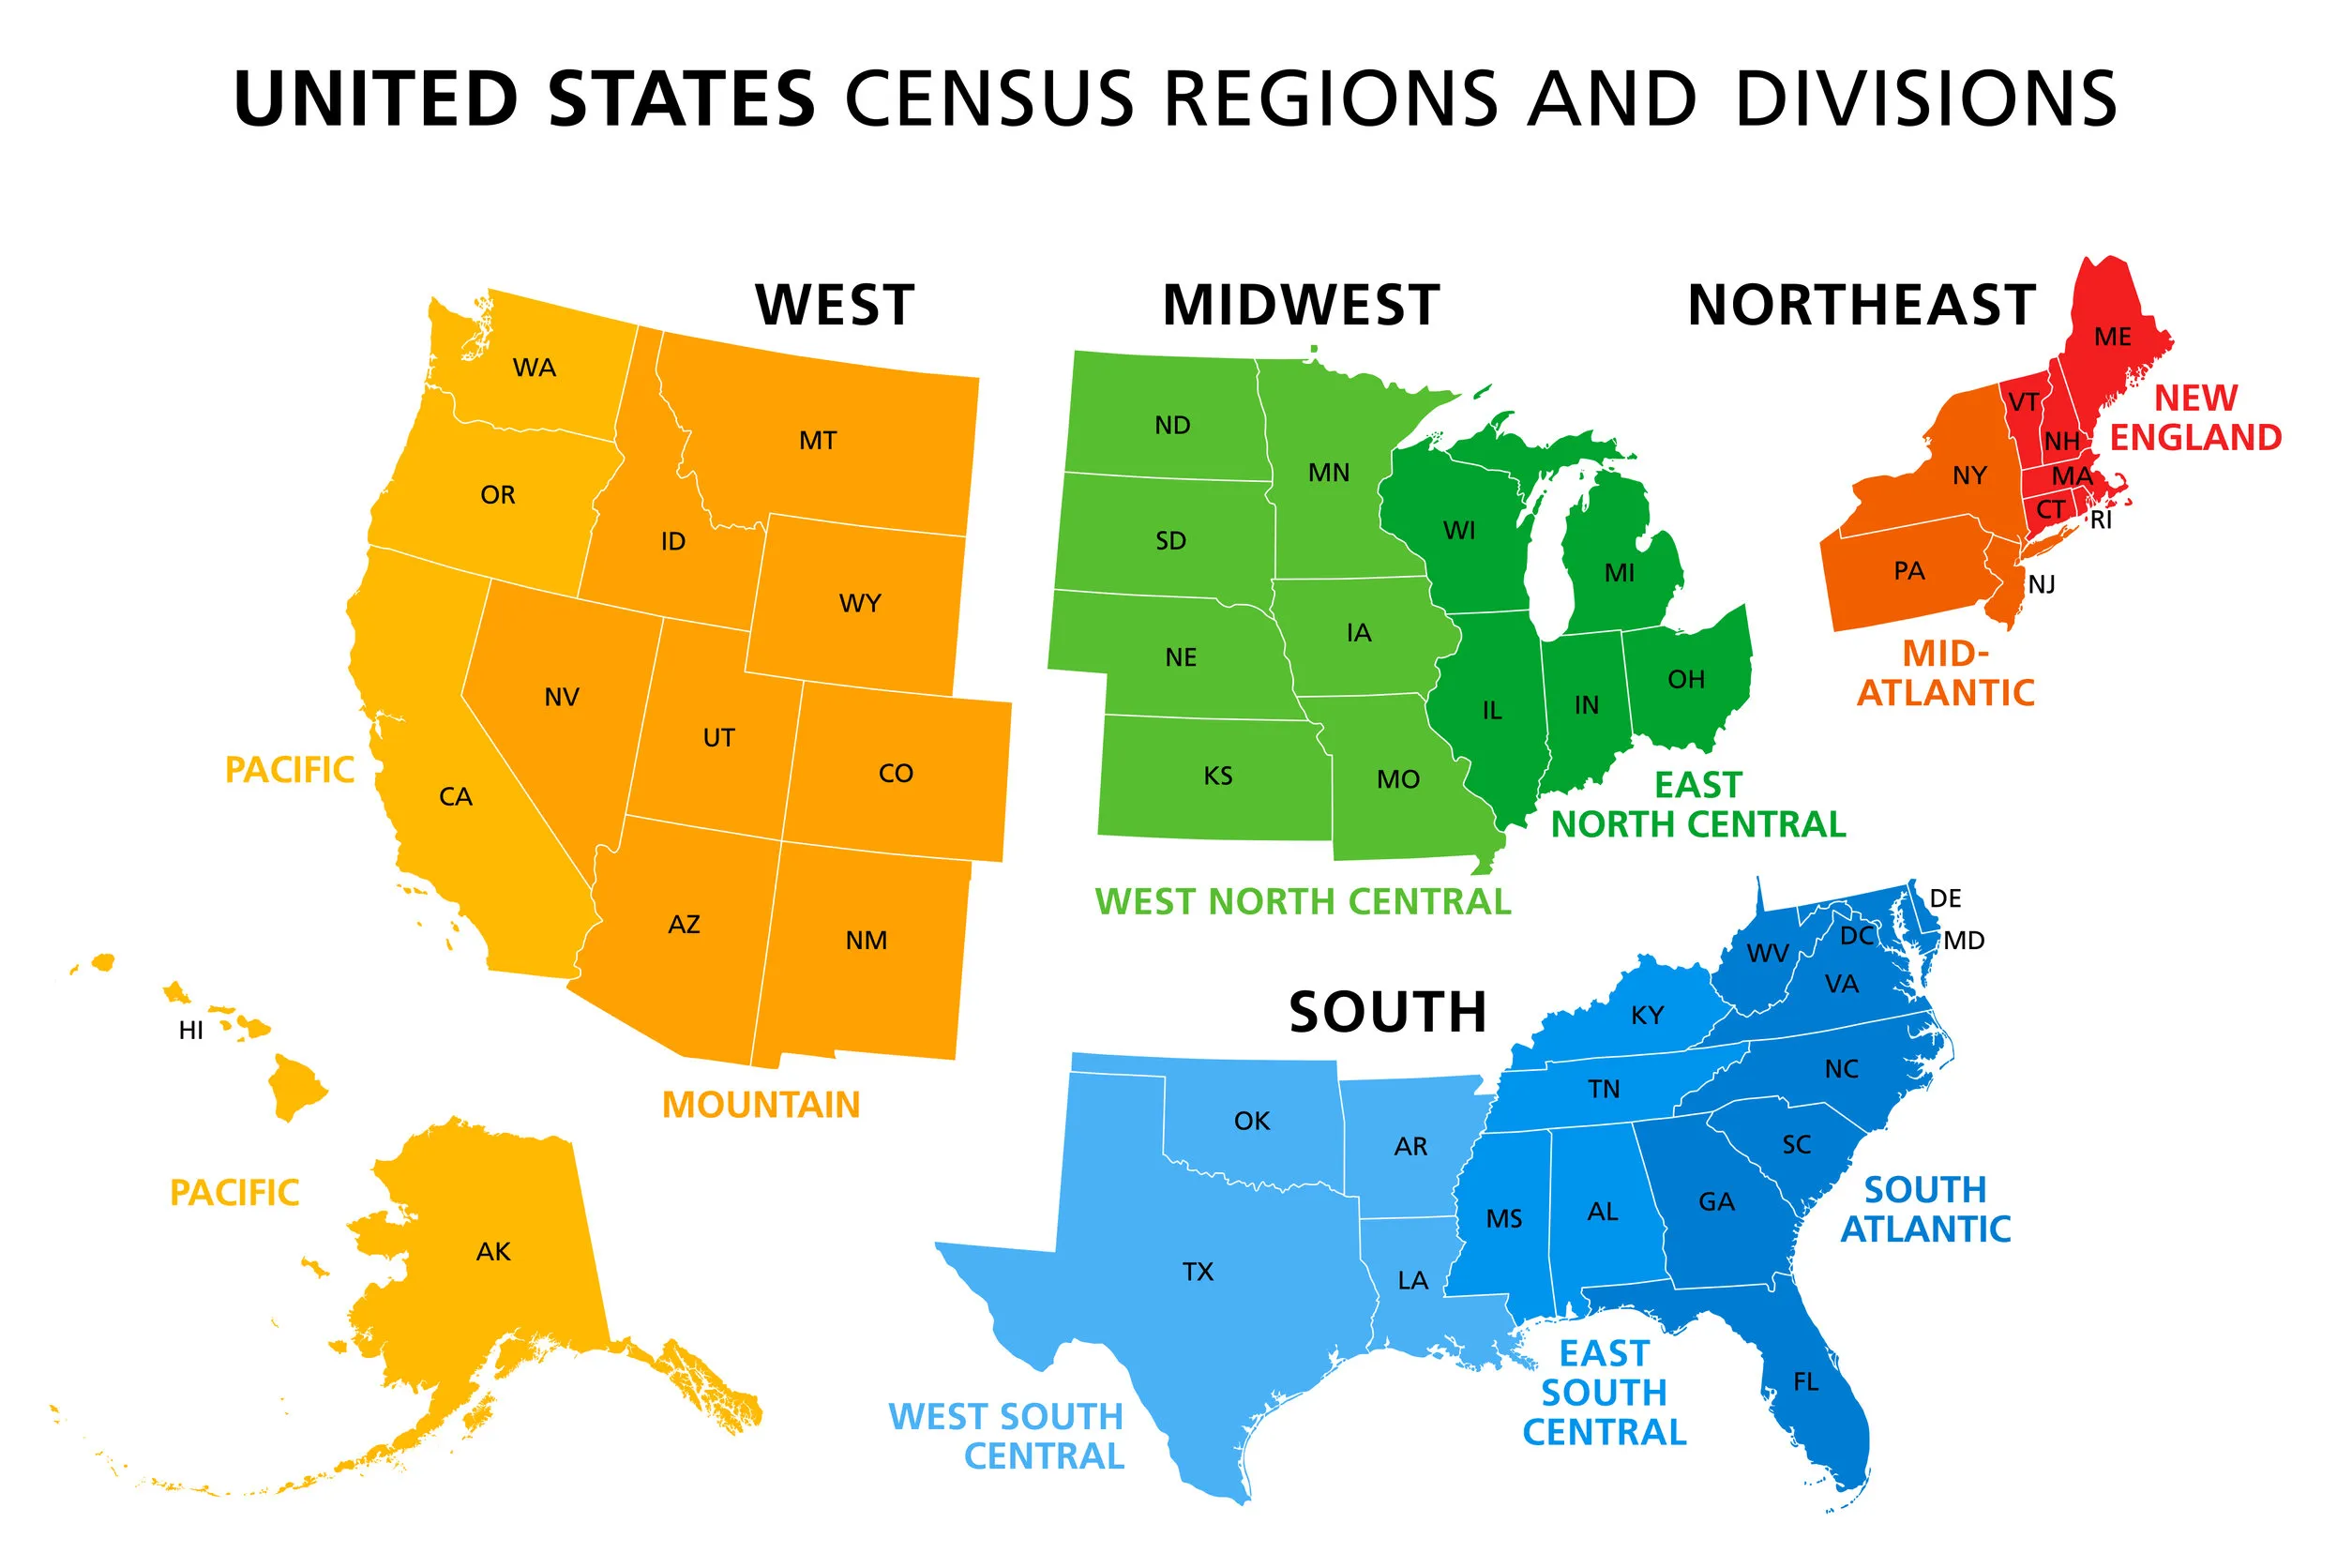
\includegraphics[scale=0.06]{figures/us_regions.png}

\end{frame}

\begin{frame}{Linear regression with a categorical predictor}
What can we do? We can use \textcolor{blue}{dummy variables}\dots

\vspace{0.3cm}

\textcolor{blue}{Dummy variables}: The set of \textit{binary} variables created by re-writing (or re-coding) a multilevel categorical variable  

\vspace{0.3cm}

Example: Suppose we have a multilevel categorical variable for US region, with values West, Midwest, South, and Northeast

\vspace{0.3cm}

We create the new variables:
\begin{itemize}
	\item Midwest: \textit{Midwest} = 1 if \textit{region} = \textit{Midwest}, and 0 otherwise
	\item South: \textit{South} = 1 if \textit{region} = \textit{South}, and 0 otherwise
	\item Northeast: \textit{Northeast} = 1 if \textit{region} = \textit{Northeast}, and 0 otherwise
\end{itemize} \pause

\vspace{0.1cm}

\textcolor{blue}{Question:} We didn't make a dummy variable for West. Why not? \pause

\medskip

\textcolor{blue}{Answer:} If all other dummy variables (Midwest, South, and Northeast) are 0, then the region must be West! In this case, West is referred to as a \textcolor{blue}{reference group}.
\end{frame} 

\begin{frame}{Linear regression with a categorical predictor}
Writing out our regression model for this example, we have
$$
E[\text{Outcome} \mid \text{Region}] = \beta_0 + \beta_1 \times \text{Midwest} + \beta_2 \times \text{South} + \beta_3 \times \text{Northeast}
$$

Note that we have more than just an intercept and slope coefficient here (making our way towards multiple linear regression!)

\vspace{0.3cm}

\textcolor{blue}{Question}: How do we interpret the coefficients $\beta_0$, $\beta_1$, $\beta_2$, $\beta_3$? \pause

\vspace{0.3cm}

$\beta_0$: average outcome among those in the Western region

$$
E[\text{Outcome} \mid \text{Region = West}] = \beta_0 + \beta_1 \times 0 + \beta_2 \times 0 + \beta_3 \times 0
$$


\end{frame}

\begin{frame}{Linear regression with a categorical predictor}
Writing out our regression model for this example, we have
$$
E[\text{Outcome} \mid \text{Region}] = \beta_0 + \beta_1 \times \text{Midwest} + \beta_2 \times \text{South} + \beta_3 \times \text{Northeast}
$$

Note that we have more than just an intercept and slope coefficient here (making our way towards multiple linear regression!)

\vspace{0.3cm}

\textcolor{blue}{Question}: How do we interpret the coefficients $\beta_0$, $\beta_1$, $\beta_2$, $\beta_3$?

\vspace{0.3cm}

$\beta_1$: difference in average outcome between groups in the Western region and Midwest region

\begin{align*}
E[&\text{Outcome} \mid  \text{Region = Midwest}] - E[\text{Outcome} \mid \text{Region = West}] \\
& = [\beta_0 + \beta_1 \times 1 + \beta_2 \times 0 + \beta_3 \times 0] - [\beta_0 + \beta_1 \times 0 + \beta_2 \times 0 + \beta_3 \times 0] \\
& = \beta_0 + \beta_1 - \beta_0 \\
& = \beta_1
\end{align*}


\end{frame}

\begin{frame}{Linear regression with a categorical predictor}
Writing out our regression model for this example, we have
$$
E[\text{Outcome} \mid \text{Region}] = \beta_0 + \beta_1 \times \text{Midwest} + \beta_2 \times \text{South} + \beta_3 \times \text{Northeast}
$$

Note that we have more than just an intercept and slope coefficient here (making our way towards multiple linear regression!)

\vspace{0.3cm}

\textcolor{blue}{Question}: How do we interpret the coefficients $\beta_0$, $\beta_1$, $\beta_2$, $\beta_3$?

\vspace{0.3cm}

$\beta_2$: difference in average outcome between groups in the Western region and Southern region

\begin{align*}
E[&\text{Outcome} \mid  \text{Region = South}] - E[\text{Outcome} \mid \text{Region = West}] \\
& = [\beta_0 + \beta_1 \times 0 + \beta_2 \times 1 + \beta_3 \times 0] - [\beta_0 + \beta_1 \times 0 + \beta_2 \times 0 + \beta_3 \times 0] \\
& = \beta_0 + \beta_2 - \beta_0 \\
& = \beta_2
\end{align*}


\end{frame}

\begin{frame}{Linear regression with a categorical predictor}
Writing out our regression model for this example, we have
$$
E[\text{Outcome} \mid \text{Region}] = \beta_0 + \beta_1 \times \text{Midwest} + \beta_2 \times \text{South} + \beta_3 \times \text{Northeast}
$$

Note that we have more than just an intercept and slope coefficient here (making our way towards multiple linear regression!)

\vspace{0.3cm}

\textcolor{blue}{Question}: How do we interpret the coefficients $\beta_0$, $\beta_1$, $\beta_2$, $\beta_3$?

\vspace{0.3cm}

$\beta_3$: difference in average outcome between groups in the Western region and Northeastern region

\begin{align*}
E[&\text{Outcome} \mid  \text{Region = Northeast}] - E[\text{Outcome} \mid \text{Region = West}] \\
& = [\beta_0 + \beta_1 \times 0 + \beta_2 \times 0 + \beta_3 \times 1] - [\beta_0 + \beta_1 \times 0 + \beta_2 \times 0 + \beta_3 \times 0] \\
& = \beta_0 + \beta_3 - \beta_0 \\
& = \beta_3
\end{align*}

\end{frame}

\begin{frame}{Linear regression with a categorical predictor: summary}
Our example:
$$
E[\text{Outcome} \mid \text{Region}] = \beta_0 + \beta_1 \times \text{Midwest} + \beta_2 \times \text{South} + \beta_3 \times \text{Northeast}
$$

\begin{itemize}
	\item If we have $k$ categories, we create $k - 1$ \textcolor{blue}{dummy variables}, with the $k$th category being the \textcolor{blue}{reference group} captured in the intercept
	\item \texttt{R} automatically creates these dummy variables for you for multilevel categorical variables, as you'll see on your homework
\end{itemize}

\vspace{0.3cm}

Hypothesis testing: If we want to test whether our outcome is associated with a multilevel categorical variable, we need to test if \textit{all} coefficients for the dummy variables (in this example, $\beta_1, \beta_2, \beta_3$) are equal to zero.

\end{frame}

\begin{frame}{The Births Dataset}
	\vspace{-5 mm}
	
	Data containing a random sample of 2500 singleton births in King County in 2001. In 1989, Seattle and King County started a program called \href{https://kingcounty.gov/depts/health/child-teen-health/maternity-support-infant-case-management.aspx}{\textcolor{cyan}{First Steps}} which provides free pre-natal care to low-income, pregnant individuals. 
	
	\medskip
	The goal of the program is to improve birth outcomes, including increased birthweights in King County. Low infant birthweight is one of the most important factors affecting neonatal mortality. 

\medskip

Variables in the dataset include:

\medskip
\begin{itemize}
	\item Participation in First Steps (yes/no)
	\item Birth parent's age at time of birth (years)
	\item Birthweight (grams)
	\item Child's gestational age at birth (weeks)
	\item Race (Black, Hispanic, Asian, White, Other)
\end{itemize}

\vspace{0.3cm} 

\textbf{We'll refer to this dataset as the \textcolor{blue}{births} dataset.} Available on the Canvas site as \color{blue} births.csv
\end{frame}

\begin{frame}{Linear regression with a categorical predictor in \texttt{R}}
	\vspace{-7 mm}
	
Suppose we're interested in whether birthweight is associated with race (Black, Hispanic, Asian, White, Other). We can fit a linear regression model as before with simple linear regression.
\medskip

\textcolor{violet}{Pollev:} Which is our reference group?

\vspace{0.3cm}

\centering

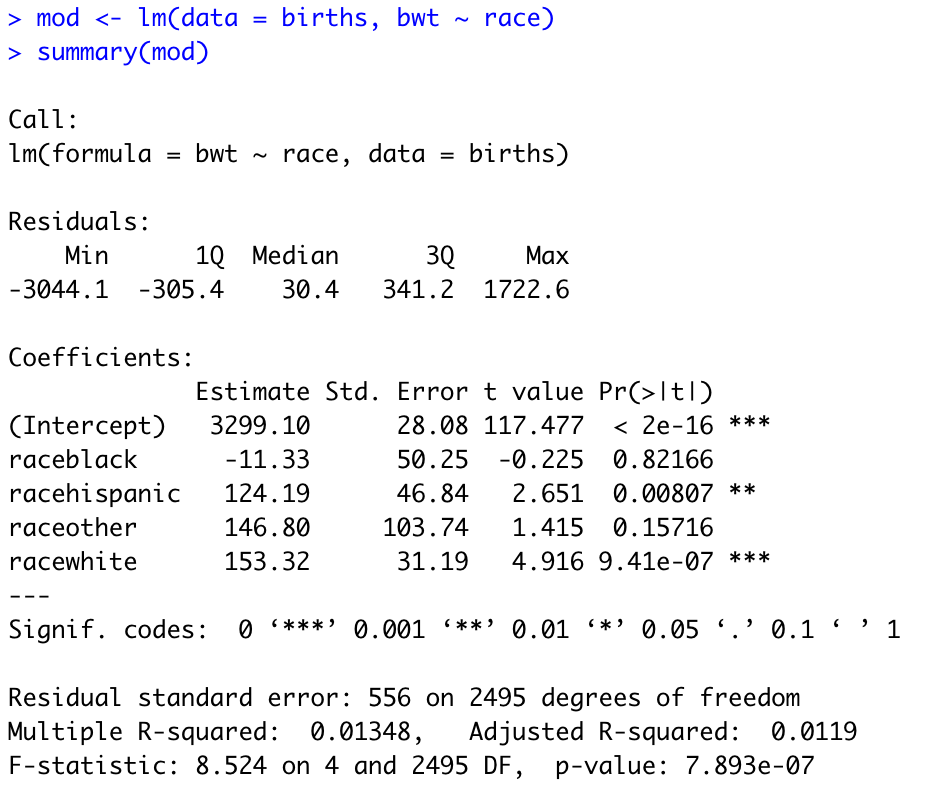
\includegraphics[scale=0.4]{figures/multilevel_cat_lm.png}


\smallskip
\raggedright
\scriptsize{\url{https://PollEv.com/multiple_choice_polls/DGHlN0vHZg24IHXNu5HYB/respond}}

\end{frame}


\begin{frame}{Linear regression with a categorical predictor in \texttt{R}}

\begin{figure}
	\centering 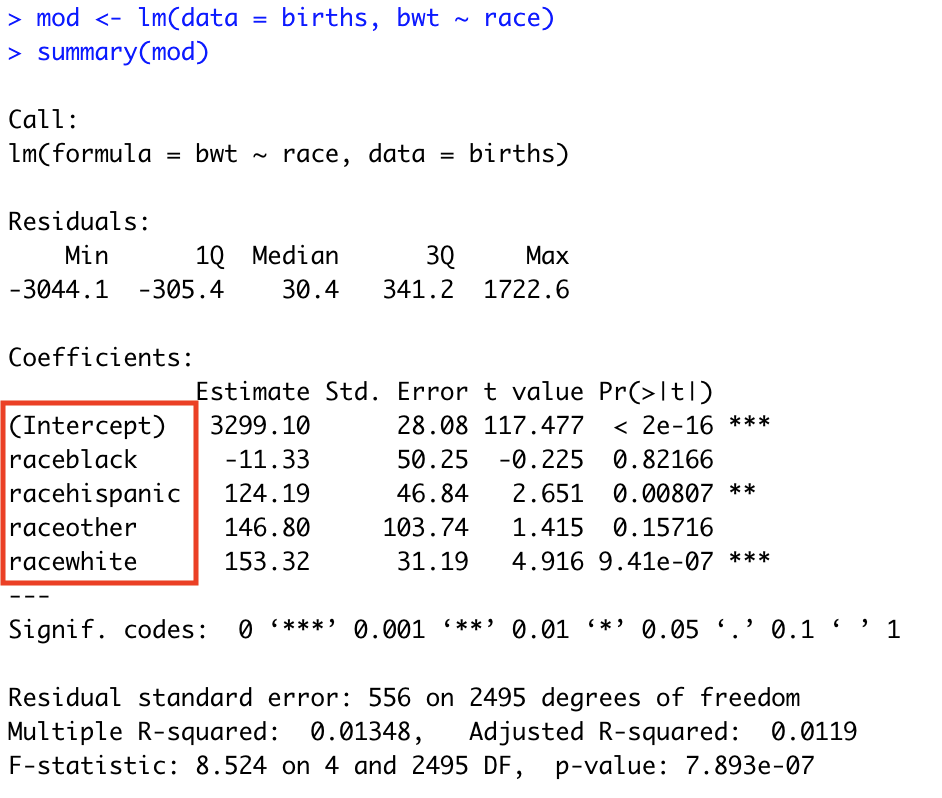
\includegraphics[scale=0.3]{figures/multilevel_cat_lm2.png}
\end{figure}

\vspace{0.1cm}

A couple things to notice:
\begin{itemize}
	\item \texttt{R} has created dummy variables for us! The reference group by default will be the first category alphabetically (in this case, ``\texttt{asian}").
\end{itemize}

\end{frame}

\begin{frame}{Linear regression with a categorical predictor in \texttt{R}}

\begin{figure}
	\centering 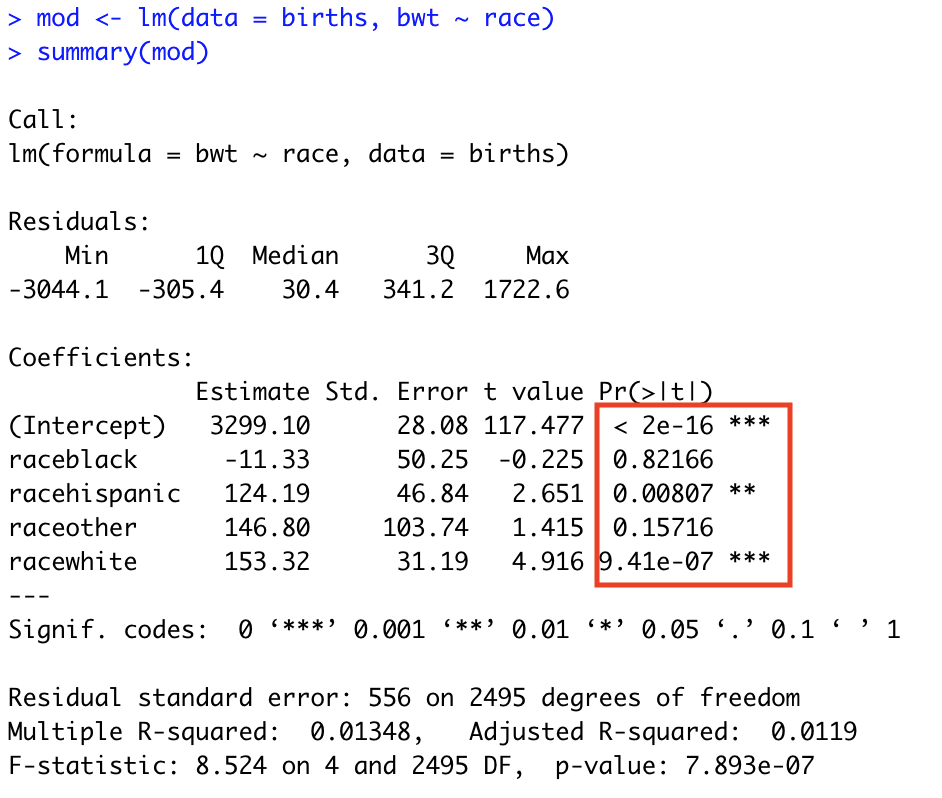
\includegraphics[scale=0.3]{figures/multilevel_cat_lm3.png}
\end{figure}

\vspace{0.1cm}

A couple things to notice:
\begin{itemize}
	\item We have multiple p-values! But which p-value is the one associated with our hypothesis test? Let's write it down\dots
\end{itemize}

\end{frame}

\begin{frame}{Linear regression with a categorical predictor in \texttt{R}}
We're interested in whether birthweight is associated with race, in our \texttt{births} dataset. Our regression model has the form:
$$
E[\texttt{bwt} \mid \texttt{race}] = \beta_0 + \beta_1 \times \texttt{black} + \beta_2 \times \texttt{hispanic} + \beta_3 \times \texttt{other} + \beta_4 \times \texttt{white}
$$ \pause

Our null hypthesis (in words) is that there is no association between race and birthweight. This would mean that \textcolor{blue}{all coefficients for dummy variables for race} are \textit{simultaneously} equal to zero. \pause In math:

\vspace{0.3cm}

\begin{itemize}
	\item $H_0$: $\beta_1 = \beta_2 = \beta_3 =\beta_4 =  0$
	\item $H_1$: \textit{at least one} of $\beta_1, \beta_2, \beta_3, \beta_4$ is not equal to $0$
\end{itemize} \pause

\vspace{0.3cm}

How do we do this in \texttt{R}?

\end{frame}

\begin{frame}{Linear regression with a categorical predictor in \texttt{R}}
In \texttt{R}, we create two linear regression models: one with the race variable and an intercept, and one with only an intercept. We then use the \texttt{anova} function to test whether the race variable as a whole is significantly associated with birthweight.

\vspace{0.3cm}

\texttt{mod1 <- lm(data = df, bwt} $\sim$ \texttt{1) \\
	mod2 <- lm(data = df, bwt} $\sim$ \texttt{race) \\
	anova(mod1, mod2)} \pause

\vspace{0.3cm}

Details:
\begin{itemize}
	\item \texttt{mod1} is the model with only an intercept (specified with the $1$ on the right hand side of the tilde)
	\item Inside of the \texttt{anova} function, we put the ``smaller" model first (in this case, the model without the race covariate)
\end{itemize}
\end{frame}

\begin{frame}{Linear regression with a categorical predictor in \texttt{R}}

\vspace{-5 mm}

Our output from the \texttt{anova} function:

\vspace{0.15cm}

\begin{figure}
	\centering 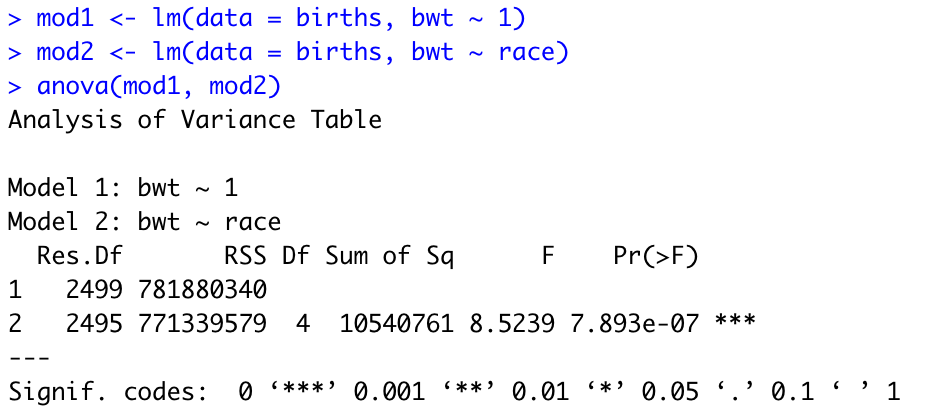
\includegraphics[scale=0.5]{figures/anova_race.png}
\end{figure}

\end{frame}

\begin{frame}{Linear regression with a categorical predictor in \texttt{R}}
	\vspace{-5mm}
	
Our output from the \texttt{anova} function:

\vspace{0.15cm}

\begin{figure}
	\centering 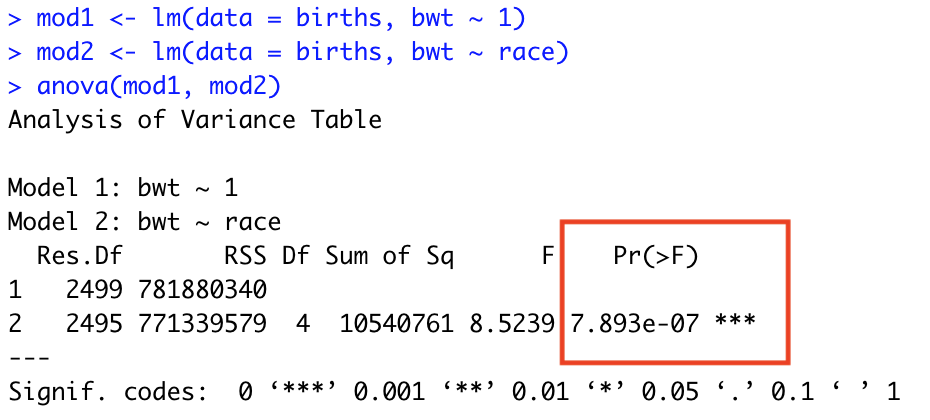
\includegraphics[scale=0.5]{figures/anova_race2.png}
\end{figure}

\vspace{0.15cm}

\textit{This} is the p-value for our hypothesis test. (The individual p-values from our linear regression output do \textit{not} correspond to the hypothesis test we want to run.) \pause

\vspace{0.3cm}



\includegraphics[scale=0.01]{figures/technical} The p-value here corresponds to an F statistic, as opposed to a $t$ statistic as with hypothesis tests for single coefficients (e.g., $\beta_1 = 0$ vs. $\beta_1 \neq 0$). The key here is that F tests allow us to test for multiple coefficients being equal to $0$ at once.

\end{frame}

\begin{frame}{Linear regression with a categorical predictor in \texttt{R}}
	\vspace{-5mm}
	
	Our output from the \texttt{anova} function:
	
	\vspace{0.15cm}
	
	\begin{figure}
		\centering 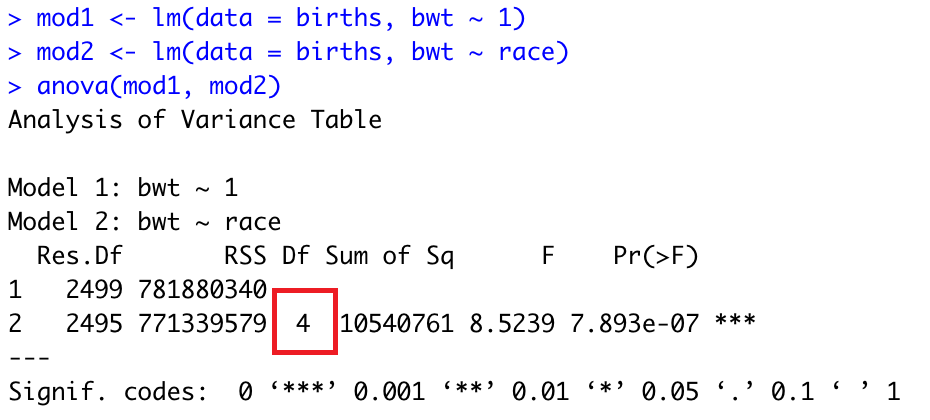
\includegraphics[scale=0.35]{figures/anova_race3.png}
	\end{figure}
	
	\vspace{0.15cm}
	
This is the degrees of freedom of our hypothesis test. The degrees of freedom are the difference in parameters between the null model (1) and the alternative model (5).
	

	
\end{frame}

\begin{frame}{\textcolor{violet}{Pollev}}
	Suppose I had a variable called location, which had levels of "Seattle", "Snoqualmie", "Redmond", and "Other". If I want to test whether location is associated with birth-weight, how many degrees of freedom will the test be? 
	
	\bigskip
	
		\url{https://PollEv.com/multiple_choice_polls/GChRpjTI2jSAMFxK98yDM/respond}\pause
	
	\bigskip
	
	\textcolor{blue}{3 degrees of freedom. There will be one parameter (an intercept) in the null model and 4 parameters in the alternative model.}
	
\end{frame}


\begin{frame}{Question}
	I can also use the anova function to compare two models for birth weight, one with just an intercept and one with the binary variable first steps participation. The p-value I get is the same as the slope p-value of the linear regression for birthweight as predicted by first steps participation. Is this surprising? Why is this?
\end{frame}

\begin{frame}{Linear regression with a categorical predictor in \texttt{R}}
Key Takeaway(s):
\vspace{0.3cm}

\begin{itemize}
	\item The individual p-values for separate categories of a multilevel categorical variable \textit{do not} correspond to the hypothesis test for whether the variable is associated with the outcome
	
	\medskip
	
	\item We use the \texttt{anova} function in \texttt{R} to get p-values that correspond to hypothesis tests where the null hypothesis involves setting \textit{more than one} coefficient equal to zero
\end{itemize} \pause

\vspace{0.3cm}

What does this example have to do with multiple linear regression? 

\vspace{0.3cm}

Multiple linear regression involves having \textit{multiple} predictors in your model. Multilevel categorical variables are a preview of multiple linear regression, as they can be framed as multiple dummy variables! \pause

\vspace{0.2cm}

*note that the polynomial transformation also involved multiple predictors in our model, so you've now had two previews of multiple linear regression

\end{frame}

\section{Adjusting for covariates}

\subsection{Motivation}

\begin{frame}{Multiple linear regression: Motivation}
So far, we have considered the relationship between the outcome $Y$ and a single covariate/predictor $X$. Some terminology we'll use now that we're dealing with multiple predictors:

\vspace{0.3cm}

\textcolor{blue}{Predictor of interest}: the covariate whose relationship to the outcome corresponds to our primary scientific/statistical question \pause

\vspace{0.3cm}

In everything we've done so far $X$ has been our predictor of interest, but it also been our \textit{only} predictor. However, there may be other variables that \textit{influence} the association between our predictor of interest and the outcome, by:

\vspace{0.3cm}

\begin{itemize}
	\item \textcolor{blue}{Confounding} the association
	\item \textcolor{blue}{Modifying} the association
	\item Providing information that \textcolor{blue}{reduces the variability} of our estimates
\end{itemize}

\end{frame}

\begin{frame}{Multiple linear regression: Motivation}
	\vspace{-5 mm}
	
(1) Suppose we collect information on the variables $X_1$ and $Y$ for 50 individuals (plotted below). What is your best guess at the linear relationship between $X_1$ and $Y$ (i.e. how would you draw the simple linear regression line on this graph)?

\vspace{0.3cm}

\centering 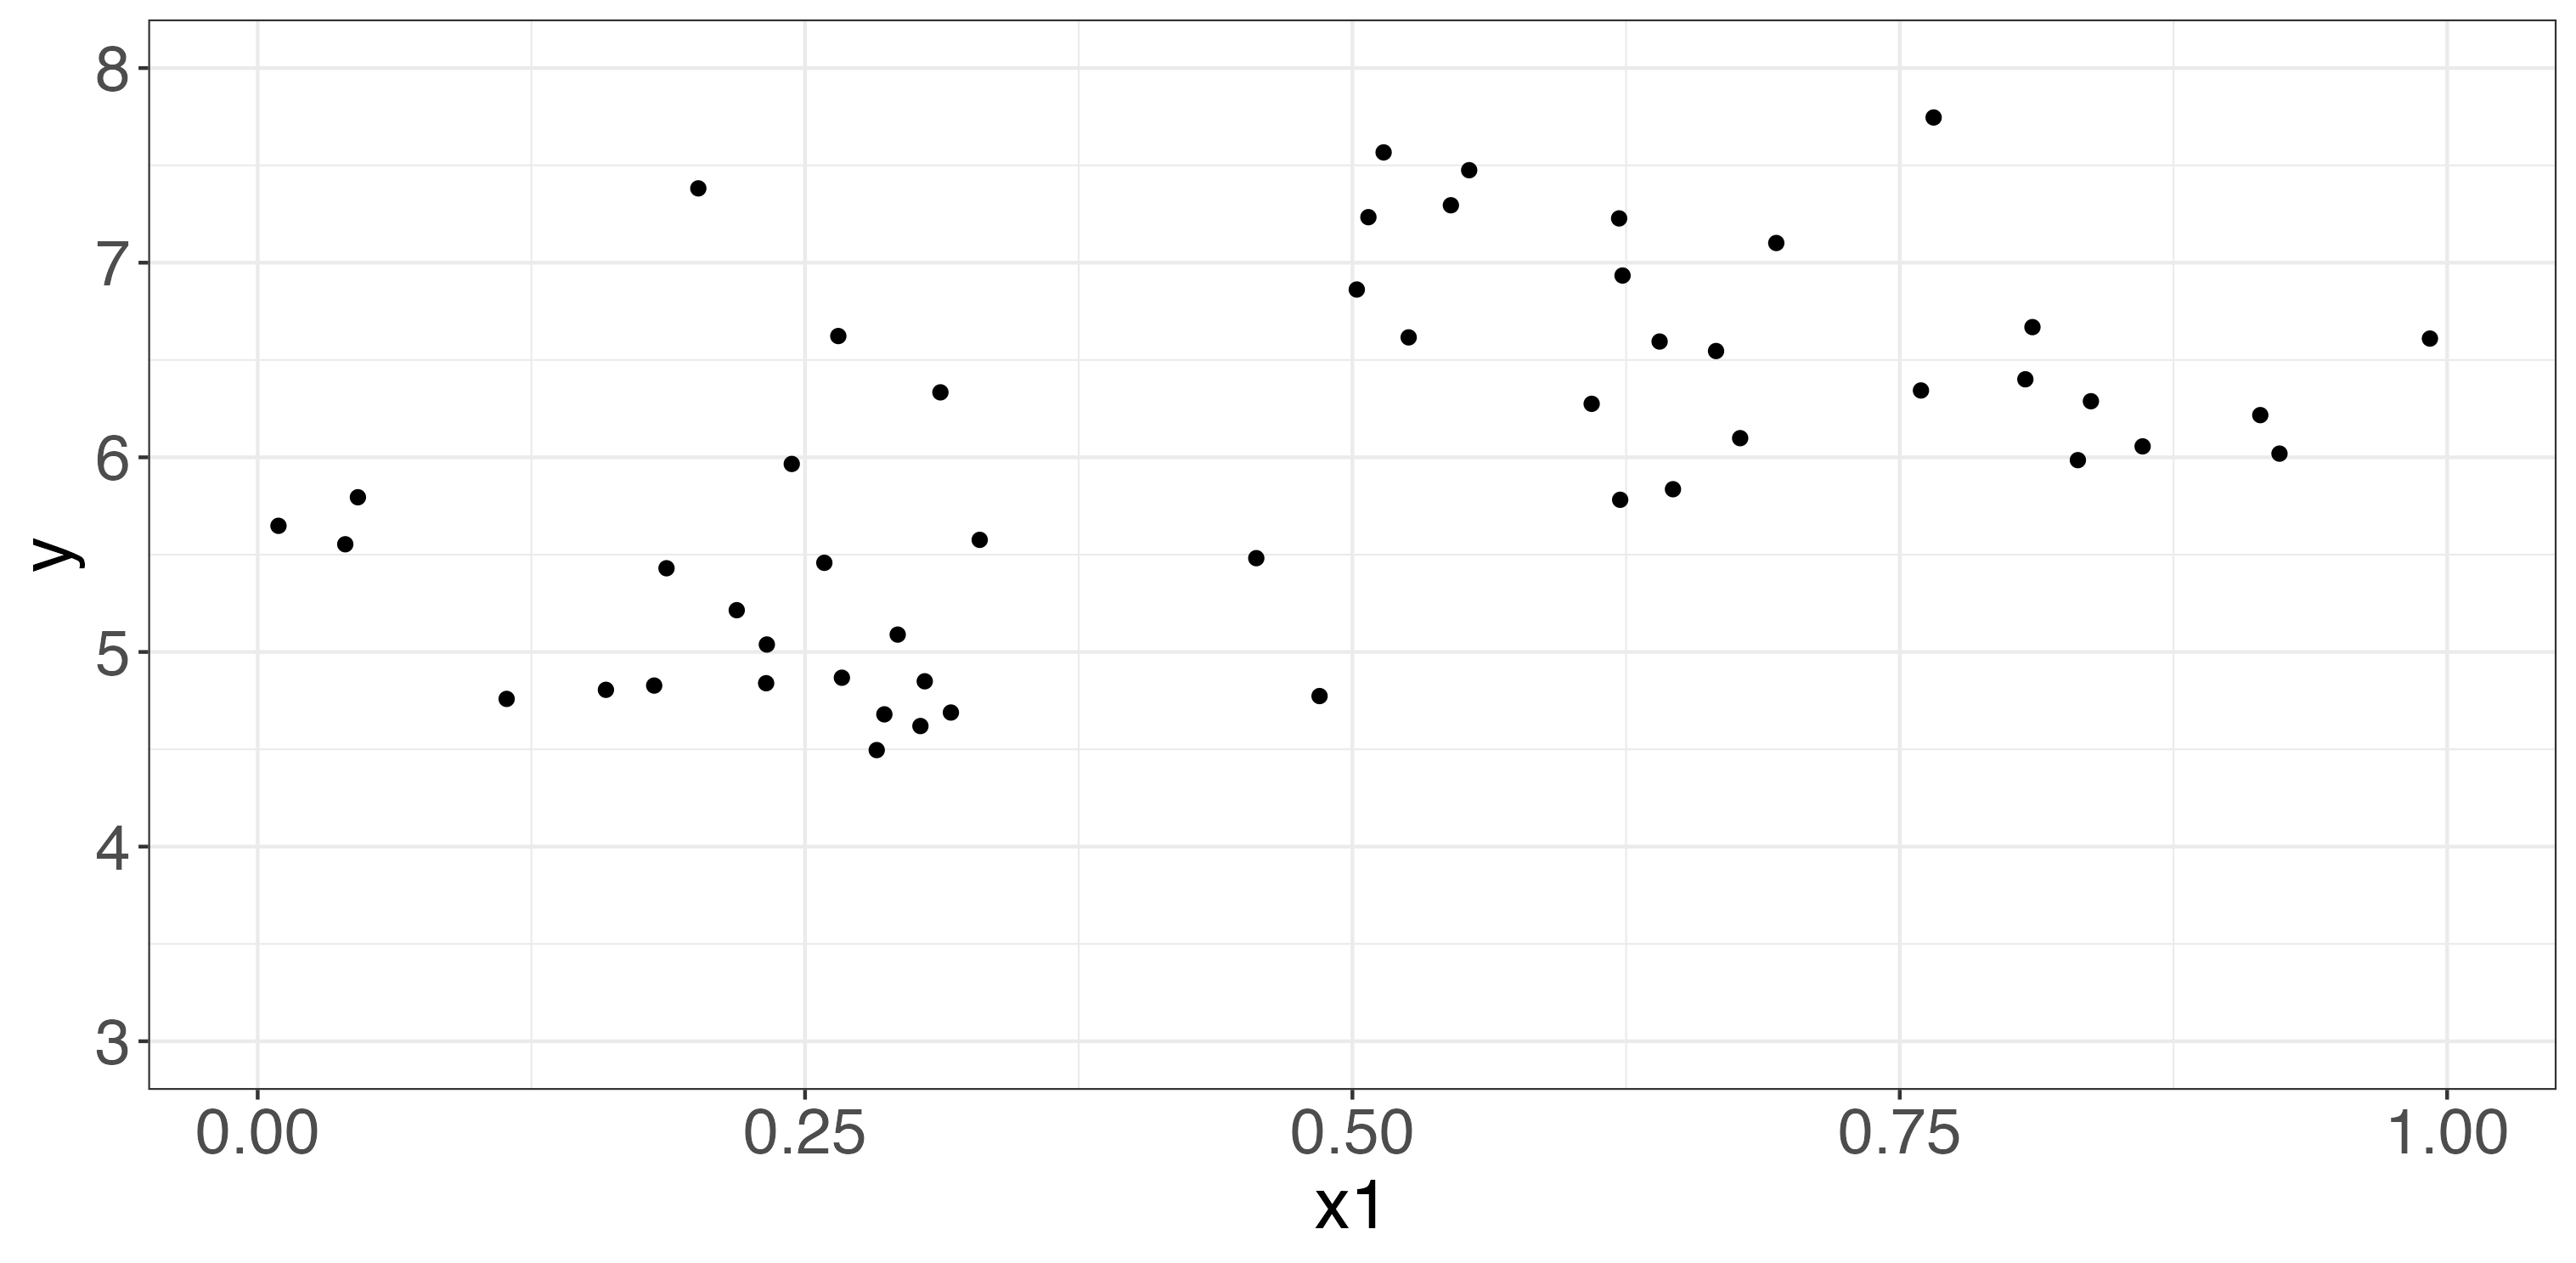
\includegraphics[scale=0.4]{figures/multreg1.png}
\end{frame}

\begin{frame}{Multiple linear regression: Motivation}
	\vspace{-5 mm}
	
(1) Suppose we collect information on the variables $X_1$ and $Y$ for 50 individuals (plotted below). What is your best guess at the linear relationship between $X_1$ and $Y$ (i.e. how would you draw the simple linear regression line on this graph)?

\vspace{0.3cm}

\centering 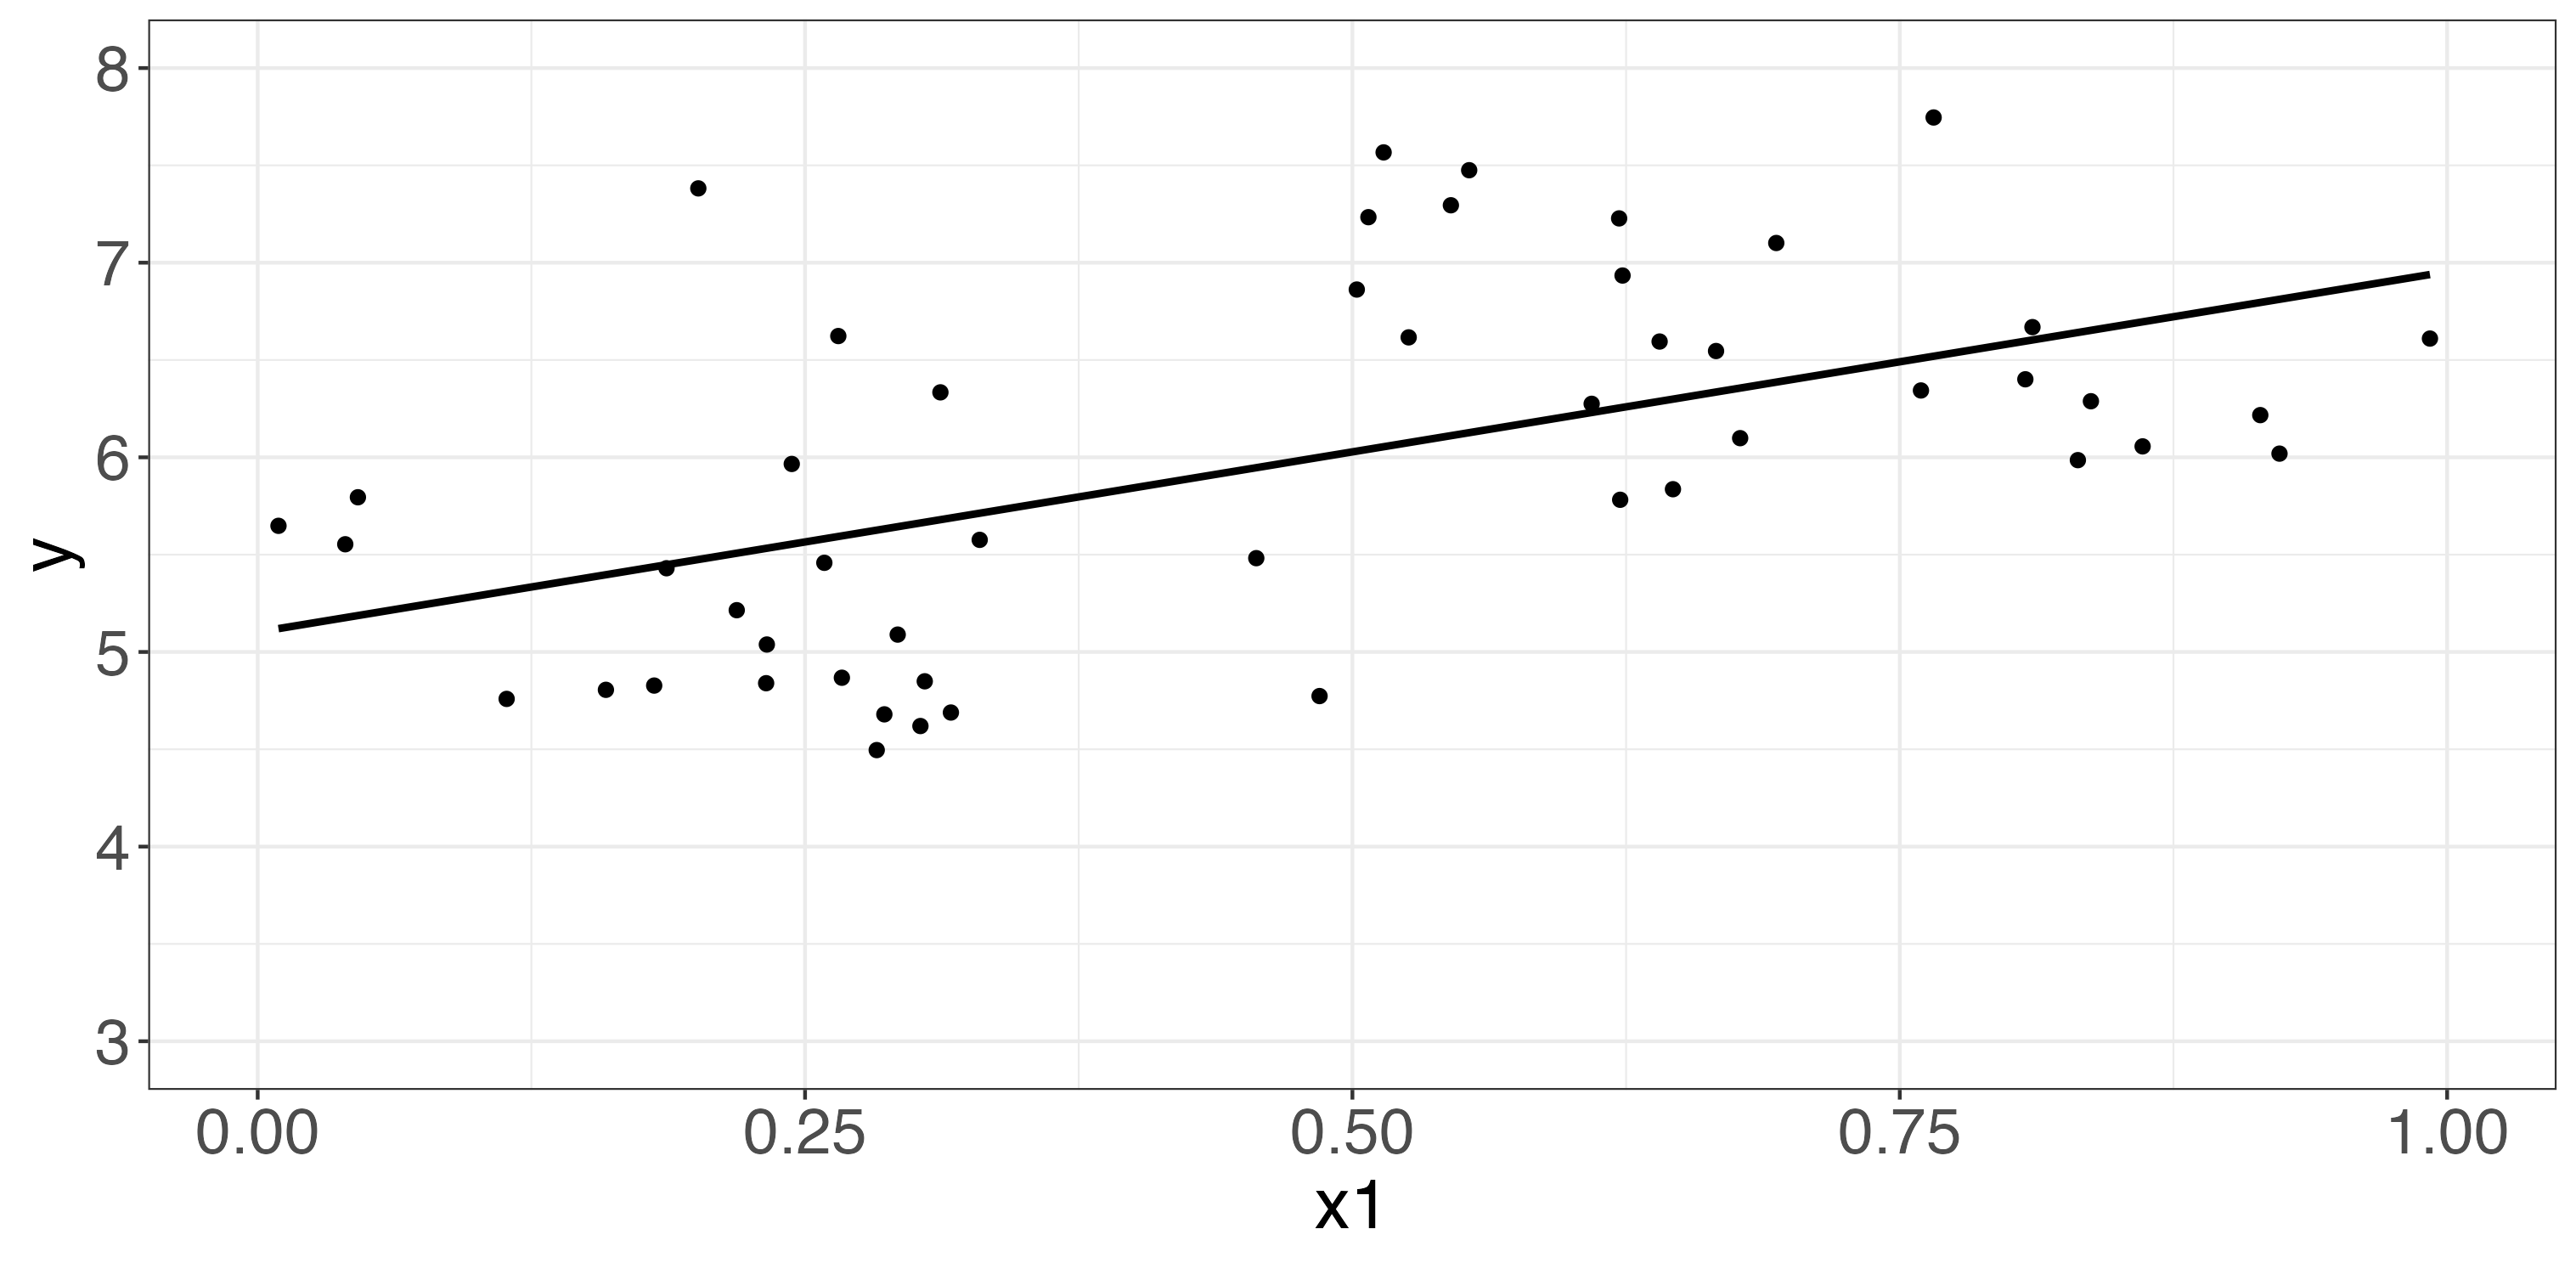
\includegraphics[scale=0.4]{figures/multreg2.png}
\end{frame}

\begin{frame}{Multiple linear regression: Motivation}
\vspace{-5 mm}

(2) Suppose we also collected information on a binary variable $X_2$ for each individual. What is your best guess at the linear relationship between $X_1$ and $Y$, \textit{for each group} defined by the variable $X_2$? 

\vspace{0.3cm}

\centering 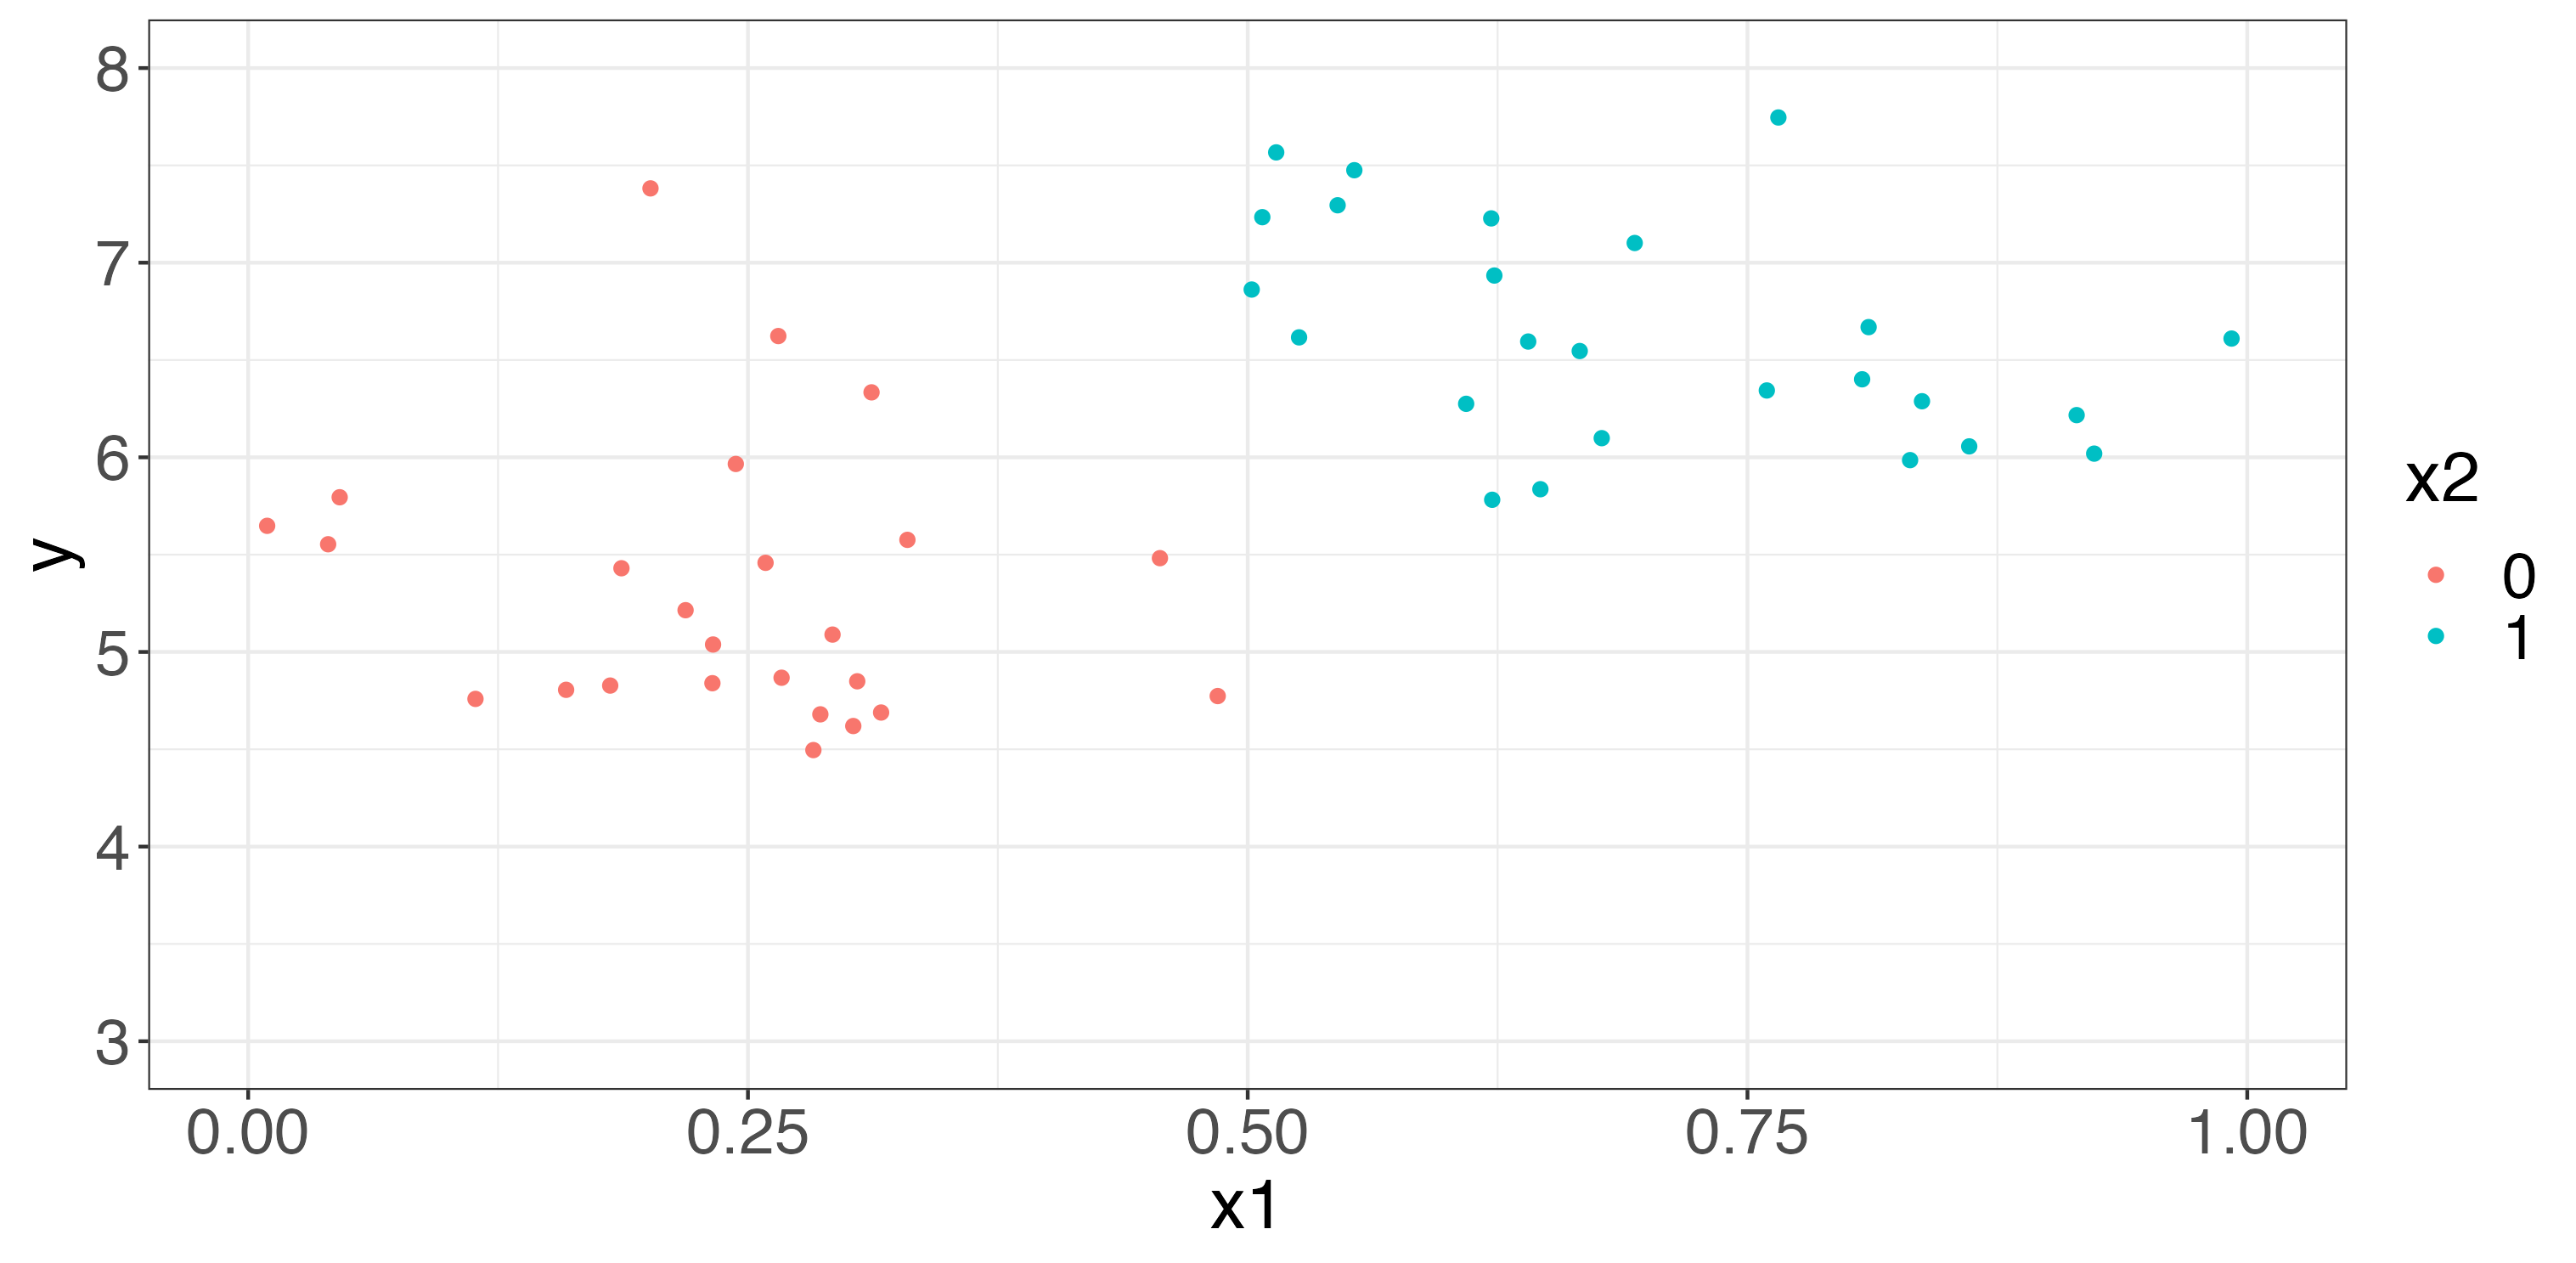
\includegraphics[scale=0.4]{figures/multreg3.png}

\end{frame}

\begin{frame}{Multiple linear regression: Motivation}
	\vspace{-5 mm}
	
(2) Suppose we also collected information on the binary variable $X_2$ for each individual. What is your best guess at the linear relationship between $X_1$ and $Y$, \textit{for each group} defined by the variable $X_2$? 

\vspace{0.3cm}

\centering 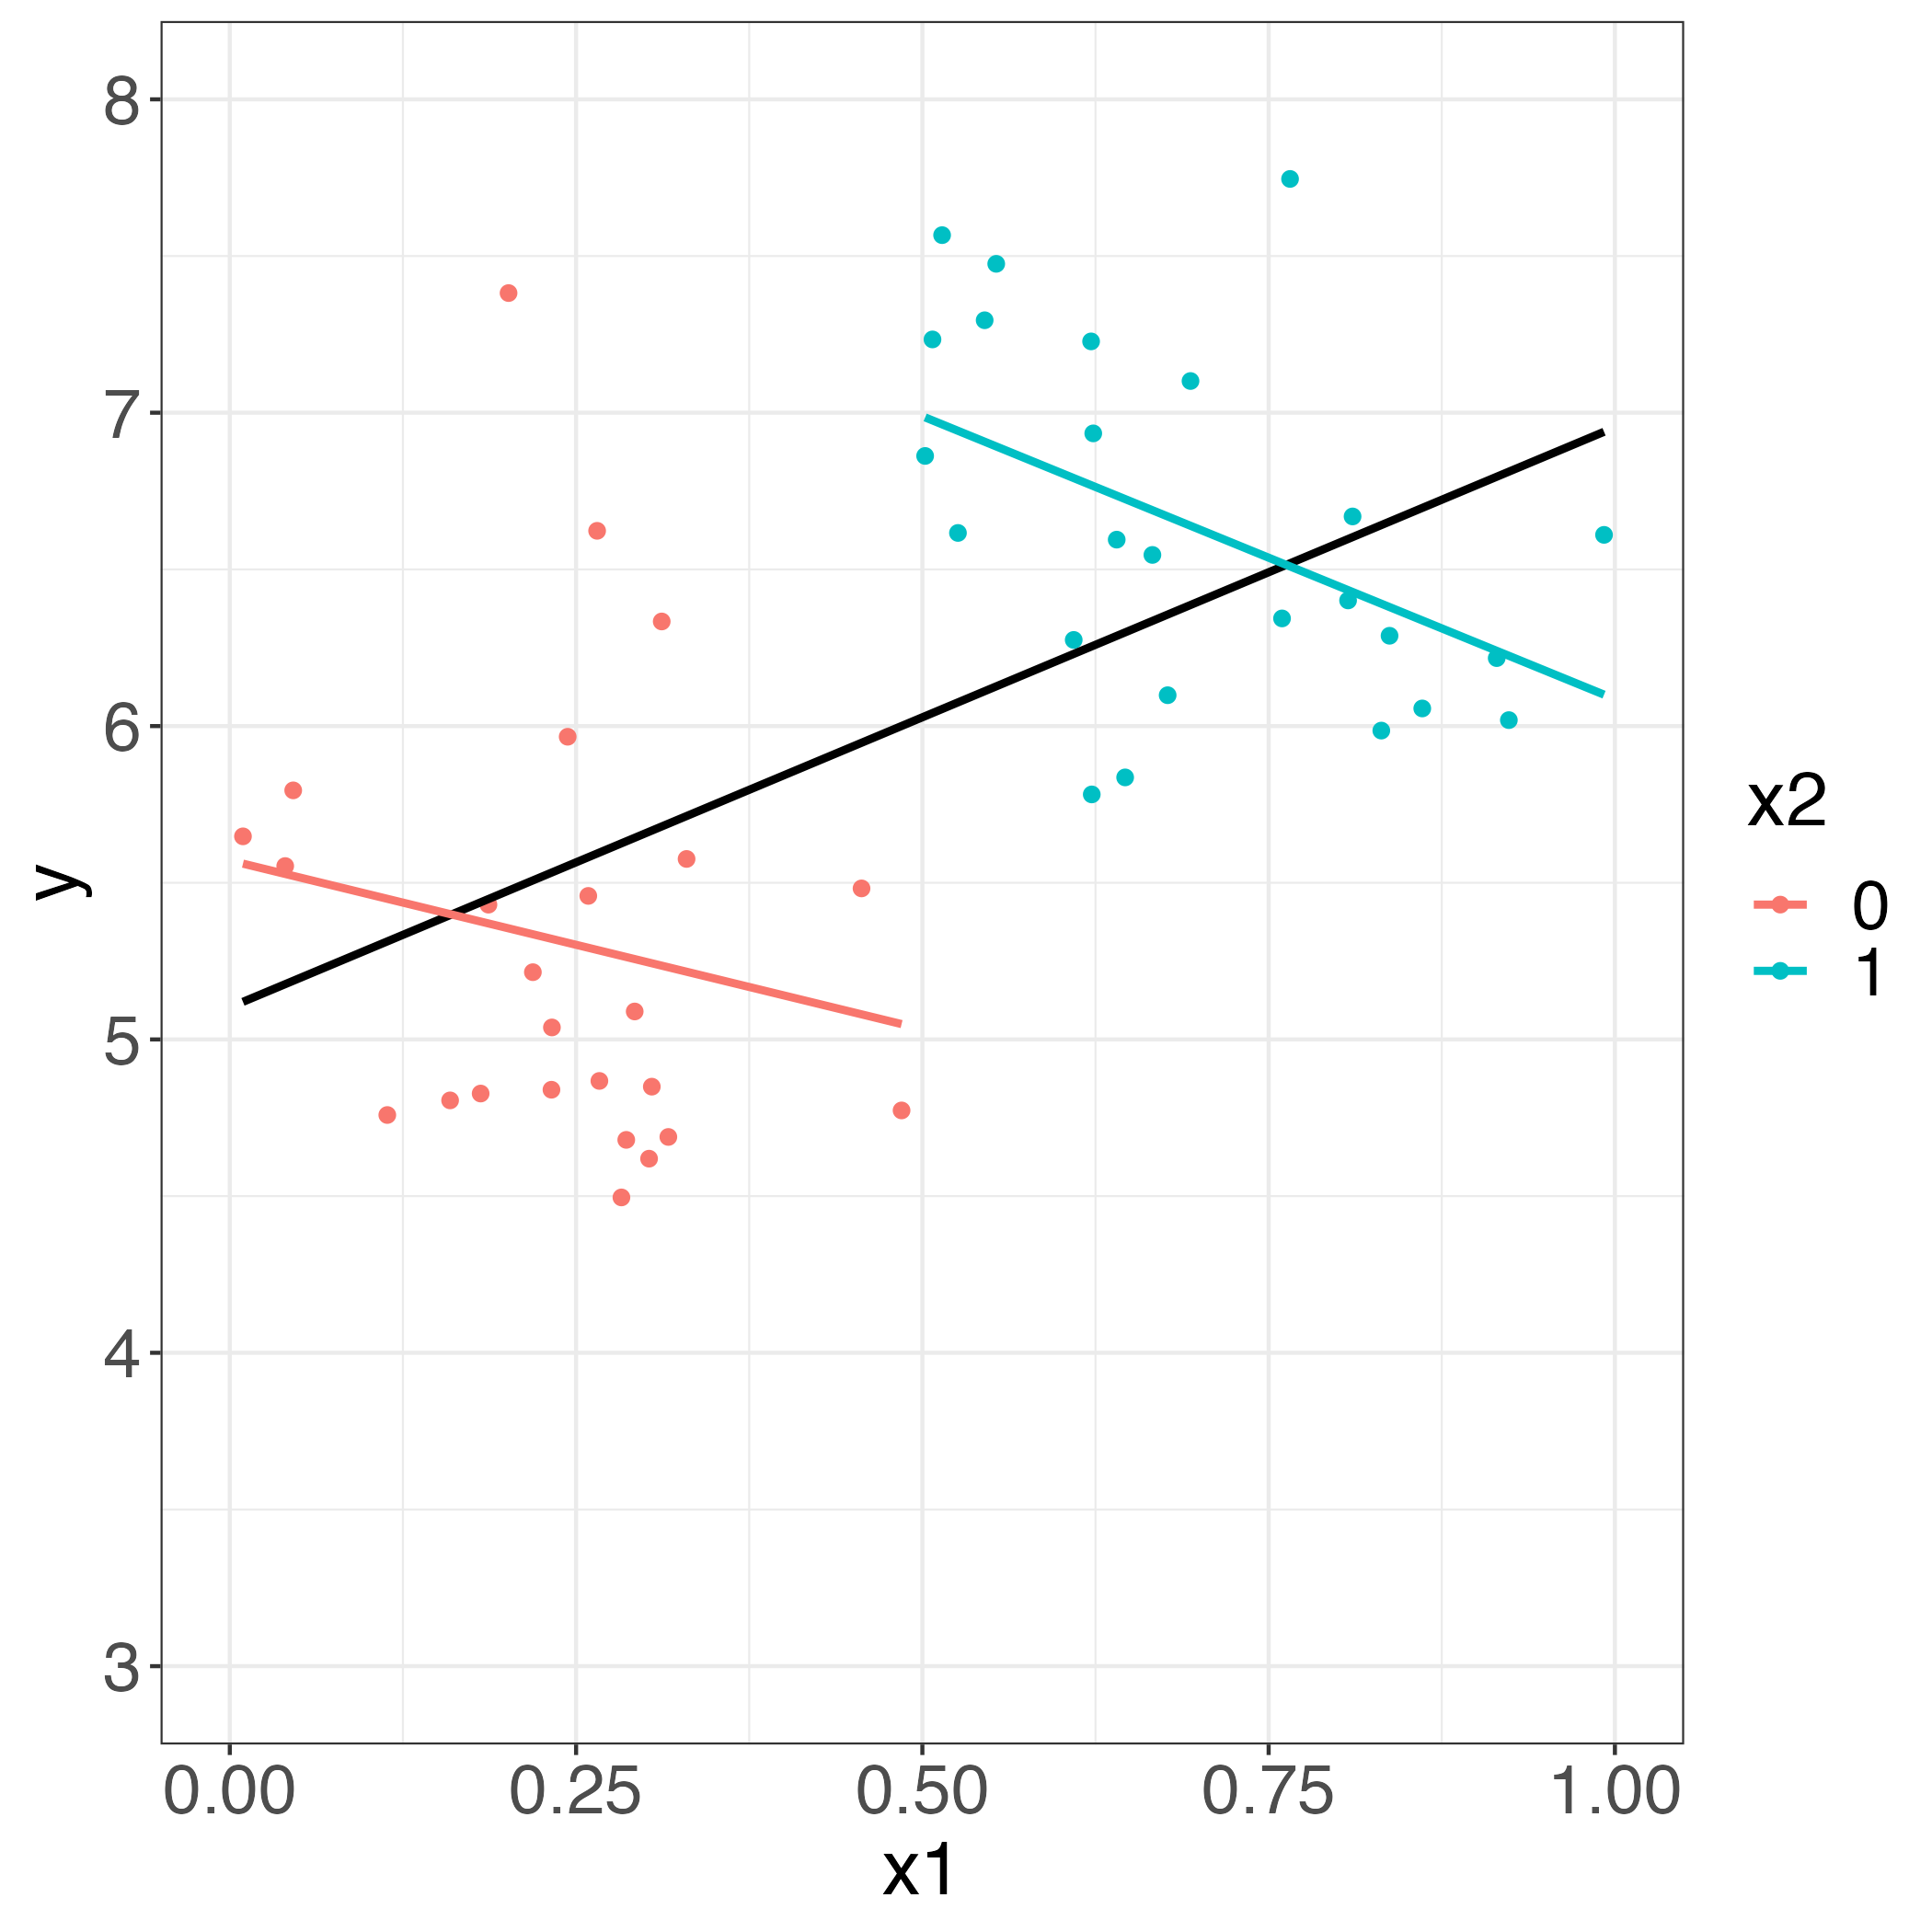
\includegraphics[scale=0.35]{figures/multreg4.png}

\end{frame}

\begin{frame}{Multiple linear regression: Motivation}
	\vspace{-0.5cm}
\begin{figure}
	\centering 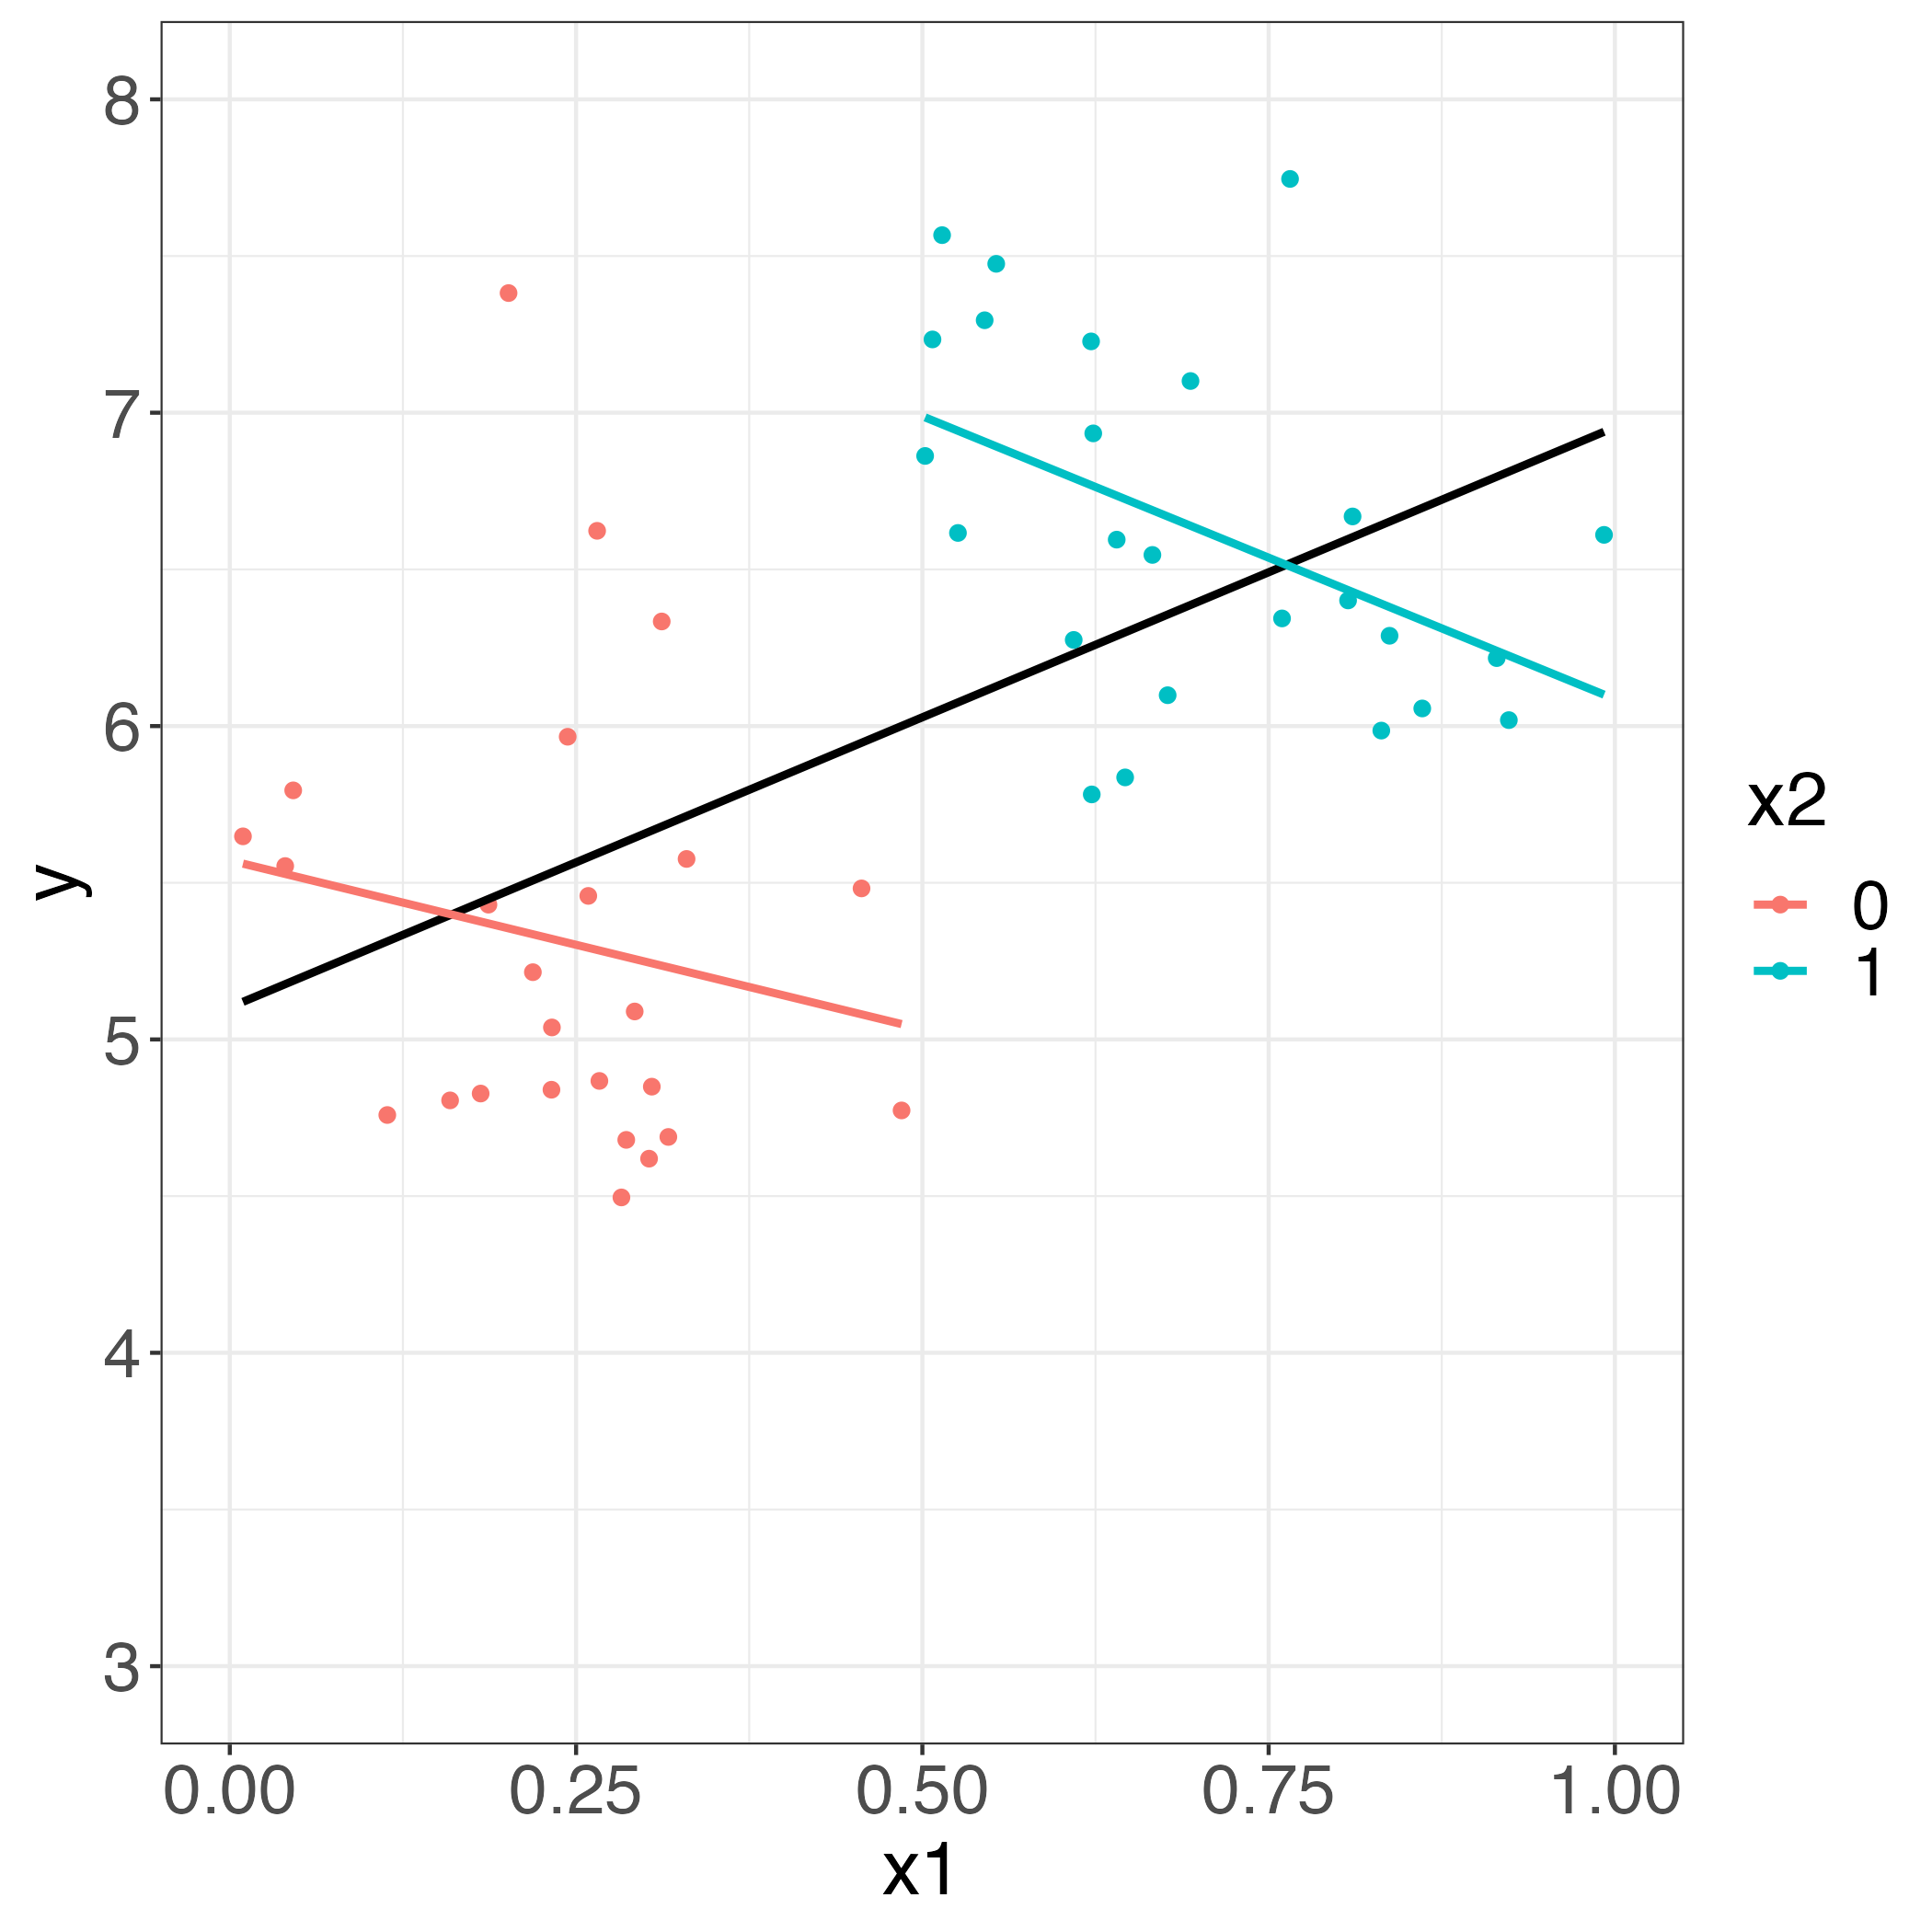
\includegraphics[scale=0.2]{figures/multreg4.png}
\end{figure}

A couple things to note:

\begin{itemize}
	\item The best fitting line between $X_1$ and $Y$ is different when we ignore $X_2$ vs. within each group defined by $X_2$
	\medskip
	
	\item The lines we drew were in response to \textit{different} questions:
	\begin{enumerate}
		\smallskip
		\item What is your best guess at the linear relationship between $X_1$ and $Y$?
		\smallskip
		\item What is your best guess at the linear relationship between $X_1$ and $Y$, \textit{within each group} defined by the variable $X_2$? 
	\end{enumerate}
\end{itemize}

\end{frame}

\begin{frame}{Multiple linear regression: Motivation}
\begin{itemize}
	\item The best fitting line between $X_1$ and $Y$ is different when we ignore $X_2$ vs. within each group defined by $X_2$
	\medskip
	
	\item The lines we drew were in response to \textit{different} questions:
	\begin{enumerate}
		\medskip
		\item What is your best guess at the linear relationship between $X_1$ and $Y$?
		\medskip
		\item What is your best guess at the linear relationship between $X_1$ and $Y$, \textit{within each group} defined by the variable $X_2$? 
	\end{enumerate}
\end{itemize}

\vspace{0.3cm}

Multiple linear regression addresses questions like the latter, where we are interested in the relationship between an outcome and a \textbf{\textcolor{blue}{predictor of interest}}, while other variables may \textcolor{blue}{influence} the association between the predictor of interest and the outcome. \pause

\vspace{0.3cm}

This is just one example of how the relationship between the outcome and predictor of interest may vary based on another variable! You may see more or less extreme differences in practice, and we'll more specific examples in the rest of the chapter.
\end{frame}


\begin{frame}{Multiple linear regression: Motivation}
	In what situations would we want / need to include additional covariates in our regression model?
	
	\vspace{0.3cm}
	
	Scientific questions typically address one of three questions about the relationship between the predictor of interest and the outcome:
	
	\vspace{0.3cm}
	
	\begin{itemize}
		\item Does the predictor of interest \textcolor{blue}{causally} effect the outcome?
		\item Is there an association between the predictor of interest and the outcome?
		\item Does the association (if it exists) \textcolor{blue}{differ in groups} defined by an additional covariate?
	\end{itemize} \pause
	
	\vspace{0.3cm}
	
	Depending on the \textcolor{blue}{study design} and \textcolor{blue}{scientific question}, we may need to include additional covariates in our model to answer these questions!
	
\end{frame}

\subsection{Multiple Linear Regression Models}

\begin{frame}{Multiple Linear Regression Models}
In simple linear regression, we modeled the expected value of $Y$ given a single predictor of interest $X_1$ as a linear function of the intercept and slope:

$$
E[Y \mid X_1] = \beta_0 + \beta_1 X_1
$$
\pause
In multiple linear regression, we'll start to add additional variables into our model. We will often call these additional variables \textcolor{blue}{covariates}. If we have a covariate $X_2$ that we want to include in our model, our regression form becomes

$$
E[Y \mid X_1, X_2] = \beta_0 + \beta_1 X_1 + \beta_2 X_2
$$

\end{frame}

\begin{frame}{Multiple Linear Regression Models}
In simple linear regression, we modeled the expected value of $Y$ given a single predictor of interest $X_1$ as a linear function of the intercept and slope:

$$
E[Y \mid X_1] = \beta_0 + \beta_1 X_1
$$
In multiple linear regression, we'll start to add additional variables into our model. We will often call these additional variables \textcolor{blue}{covariates}. If we have a covariate $X_2$ that we want to include in our model, our regression form becomes

$$
E[Y \mid X_1, \textcolor{red}{X_2}] = \beta_0 + \beta_1 X_1 + \beta_2 X_2
$$

We've included \textcolor{red}{$X_2$} on the left-hand side of our equation, because our expected outcome now depends on both $X_1$ \textit{and} $X_2$.

\end{frame}

\begin{frame}{Multiple Linear Regression Models}
In simple linear regression, we modeled the expected value of $Y$ given a single predictor of interest $X_1$ as a linear function of the intercept and slope:

$$
E[Y \mid X_1] = \beta_0 + \beta_1 X_1
$$
In multiple linear regression, we'll start to add additional variables into our model. We will often call these additional variables \textcolor{blue}{covariates}. If we have a covariate $X_2$ that we want to include in our model, our regression form becomes

$$
E[Y \mid X_1, X_2] = \beta_0 + \beta_1 X_1 + \color{red}{\beta_2 X_2}
$$

We've \textit{added} \textcolor{red}{$X_2$} to the right-hand side of our equation because with linear regression, our expected outcome is a \textit{linear combination} of predictors (this means we always add!). Note that $X_2$ also gets its own coefficient, $\beta_2$.

\end{frame}

\begin{frame}{Multiple Linear Regression Models}
In simple linear regression, we modeled the expected value of $Y$ given a single predictor of interest $X_1$ as a linear function of the intercept and slope:

$$
E[Y \mid X_1] = \beta_0 + \beta_1 X_1
$$
In multiple linear regression, we'll start to add additional variables into our model. We will often call these additional variables \textcolor{blue}{covariates}. If we have a covariate $X_2$ that we want to include in our model, our regression form becomes

$$
E[Y \mid X_1, X_2] = \beta_0 + \beta_1 X_1 + \beta_2 X_2
$$

\textcolor{blue}{Question}: What if we want to include covariates $X_3, X_4, \dots, X_{100}$ in our model as well? What would the regression equation look like?
\end{frame}

\begin{frame}{Multiple Linear Regression Models}
\textcolor{blue}{Question}: What if we want to additionally include covariates $X_3, X_4, \dots, X_{100}$ in our model as well? What would the regression equation look like?

\vspace{0.3cm}

\textcolor{blue}{Answer:} 

$$
E[Y \mid X_1, \dots, X_{100}] = \beta_0 + \beta_1 X_1 + \beta_2 X_2 + \dots + \beta_{100} X_{100}
$$

We include all of the covariates in our model on the left-hand side of the equation (after the conditional symbol, ``$|$"), and add all of the covariates to the right-hand side of the equation, each with their own coefficient.

\end{frame}


\begin{frame}{Multiple Linear Regression Models}
	\vspace{-5 mm}
	
Note that the inclusion of additional covariates in your model changes the scientific question that your model is answering.

\vspace{0.3cm}

With simple linear regression, the model:

\[E[Y \mid X_1] = \beta_0 + \beta_1 X_1\]

 was used to address the question, ``Is $X_1$ linearly associated with $Y$"?  \pause

\vspace{0.3cm}

With multiple linear regression, the model:

 \[E[Y \mid X_1, \dots, X_p] = \beta_0 + \beta_1 X_1 + \dots + \beta_p X_p\]

 (for $p$ total covariates), we address the question, ``Is $X_1$ linearly associated with $Y$, \textit{adjusting for covariates} $X_2$ through $X_p$?" 
\end{frame}

\begin{frame}{Multiple Linear Regression Models}
	\vspace{-5 mm}

	With multiple linear regression, the model:
	
	\[E[Y \mid X_1, \dots, X_p] = \beta_0 + \beta_1 X_1 + \dots + \beta_p X_p\]
	
	(for $p$ total covariates), we address the question, ``Is $X_1$ linearly associated with $Y$, \textit{adjusting for covariates} $X_2$ through $X_p$?" 
	
	\vspace{0.3cm}
	
	When we estimate the association between the predictor of interest and the outcome, we want to do so at \textcolor{blue}{fixed/constant values} of the additional covariates in the model. 
	
	\vspace{0.3cm}
	
	
	
	Of course, all scientific questions and interpretations should be made \textcolor{blue}{in the context of the problem}. 
\end{frame}

% HERE

\subsection{Interpretation}

\begin{frame}{Adjusting for covariates: interpretation}
Suppose we have just a single additional variable $Z$ in our model, along with a predictor of interest $X$ and an outcome $Y$:
$$
E[Y \mid X, Z] = \beta_0 + \beta_1 X + \beta_2 Z
$$\pause
How do we interpret\dots
\vspace{0.3cm}
\begin{enumerate}
	\item[] $\beta_0$
	\item[] $\beta_1$
	\item[] $\beta_2$
\end{enumerate}
\end{frame}

\begin{frame}{Adjusting for covariates: interpretation}
$$
E[Y \mid X, Z] = \beta_0 + \beta_1 X + \beta_2 Z
$$

\vspace{0.3cm}

$\beta_0$: The mean value of $Y$ when both $X$ and $Z$ are 0.

\vspace{0.3cm}

\textcolor{blue}{Why?} \pause $E[Y \mid X = 0, Z = 0] = \beta_0 + \beta_1 \times 0 + \beta_2 \times 0 = \beta_0$
\end{frame}

\begin{frame}{Adjusting for covariates: interpretation}
$$
E[Y \mid X, Z] = \beta_0 + \beta_1 X + \beta_2 Z
$$

\vspace{0.3cm}

$\beta_1$: The average difference in $Y$ comparing two groups that differ in one unit of $X$, and have \textit{the same} value $Z$.

\vspace{0.3cm}

\textcolor{blue}{Why?} \pause 

\begin{align*}
E[Y & \mid X = x + 1, Z = z] - E[Y \mid X = x, Z = z] \\
& = [\beta_0 + \beta_1(x + 1) + \beta_2 z] - [\beta_0 + \beta_1x + \beta_2 z] \\
& = [\beta_1 x + \beta_1 + \beta_2 z] - [\beta_1 x + \beta_2 z] \\
& = \beta_1
\end{align*}

\end{frame}

\begin{frame}{Adjusting for covariates: interpretation}
$$
E[Y \mid X, Z] = \beta_0 + \beta_1 X + \beta_2 Z
$$

\vspace{0.3cm}

$\beta_2$: The average difference in $Y$ comparing two groups that differ in one unit of $Z$, and have \textit{the same} value $X$.

\vspace{0.3cm}

\textcolor{blue}{Why?} \pause 

\begin{align*}
E[Y & \mid X = x, Z = z + 1] - E[Y \mid X = x, Z = z] \\
& = [\beta_0 + \beta_1 x + \beta_2 (z + 1)] - [\beta_0 + \beta_1x + \beta_2 z] \\
& = [\beta_1 x + \beta_2 z + \beta_2] - [\beta_1 x + \beta_2 z] \\
& = \beta_2
\end{align*}

\end{frame}

\begin{frame}{Adjusting for covariates: interpretation}
Now suppose we have a model with $p$ total covariates,
$$
E[Y \mid X_1, \dots, X_p] = \beta_0 + \beta_1 X_1 + \dots + \beta_p X_p
$$

\textcolor{blue}{Question:} How do you interpret $\beta_0$? \pause

\vspace{0.3cm}

\textcolor{blue}{Answer:} The mean value of $Y$ when all covariates $X_1$ through $X_p$ are $0$.
\end{frame}

\begin{frame}{Adjusting for covariates: interpretation}
Now suppose we have a model with $p$ total covariates,
$$
E[Y \mid X_1, \dots, X_p] = \beta_0 + \beta_1 X_1 + \dots + \beta_p X_p
$$

\textcolor{blue}{Question:} How do you interpret $\beta_1$? \pause

\vspace{0.3cm}

\textcolor{blue}{Answer:} The average difference in $Y$ comparing two groups that differ in one unit of $X_1$, and have the same value for covariates $X_2$ through $X_p$.
\end{frame}

\begin{frame}{Adjusting for covariates: interpretation}
Now suppose we have a model with $p$ total covariates,
$$
E[Y \mid X_1, \dots, X_p] = \beta_0 + \beta_1 X_1 + \dots + \beta_p X_p
$$

\textcolor{blue}{Question:} How do you interpret $\beta_k$ for some general $k = 2, \dots, p$? \pause

\vspace{0.3cm}

\textcolor{blue}{Answer:} The average difference in $Y$ comparing two groups that differ in one unit of $X_k$, and have the same value for all other covariates in the model. 
\end{frame}

\subsection{Example in \texttt{R}}

\begin{frame}{MRI Dataset}
	We will return to the MRI dataset for an example.
	\medskip
	
	\begin{itemize}
		\item In about 1986, a government sponsored cohort study of adults aged 65 years and older was conducted to observe the incidence of cardiovascular disease (especially heart attacks and congestive heart failure) and cerebrovascular disease (especially strokes) in older adults
		\medskip
		
		\item Generally healthy adults were randomly selected from Medicare rolls. Agreement to participate was high, and thus the sample can be regarded as a fairly accurate representation of healthy older Americans. 
		\medskip
		
		\item  This data includes only some of the variables and only 735 of the thousands of participants.
		
	\end{itemize}

\end{frame}

\begin{frame}{MRI Dataset}

Variables include:
\medskip	

\begin{itemize}
	\item \texttt{atrophy}: A measure of global brain atrophy detected on MRI. In persons with shrinking (atrophy) of the brain, certain fluid filled cavities in the cerebrum (the ventricles) become larger. From the MRI exam, a measurement of the degree of ventricular enlargement relative to predicted ventricular size was made. These measurements were then rescaled to be a number between 0 and 100, with 0 indicating no ventricular enlargement and 100 indicating the most severe degree of atrophy
	\medskip
	
	\item \texttt{age}: Participant age at time of MRI (years)
	\medskip
	
	\item \texttt{chf} Indicator of whether the participant had been diagnosed with congestive heart failure prior to MRI (0= no, 1= yes). Congestive heart failure is a condition in which the heart muscle becomes too weak to pump blood properly.
\end{itemize}
\end{frame}


\begin{frame}{Atrophy and CHF}
	Suppose we are interested in investigating the association between atrophy and congestive heart failure. We might suspect that older people are more likely to have atrophy and to have experienced congestive heart failure. We decide we want to look at the association between atrophy and congestive heart failure, adjusting for age. Our model is:
	
	
	\medskip
	
	\color{blue}\[E[\text{atrophy}|\text{age},\text{chf}]=\beta_0+\beta_1\text{chf}+\beta_2\text{age}\]
\end{frame}

\begin{frame}[fragile]{Fitting the model in \texttt{R}}
	
	\vspace{-5 mm}
	
	We can fit the model using the \texttt{R} code:
	
	\begin{lstlisting}
	mod <- lm(data = mri, atrophy ~ chf + age)
	
	summary(mod)
	confint(mod)
	\end{lstlisting}
	\begin{figure}
		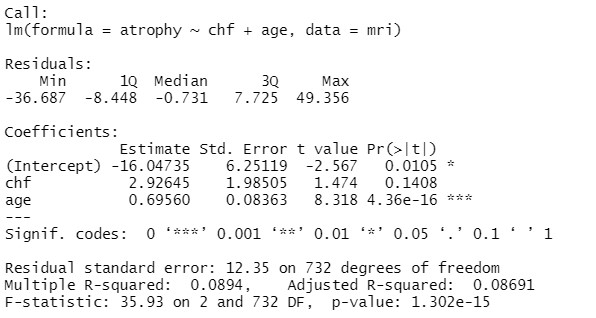
\includegraphics[scale = 0.45]{figures/mri_multiple_eg1}
		
		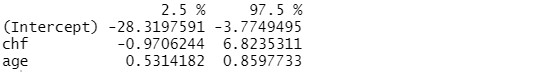
\includegraphics[scale = 0.47]{figures/mri_multiple_cis}
	\end{figure}
	
\end{frame}

\begin{frame}{\textcolor{violet}{Pollev}}
	\vspace{-5 mm}
	
	At a 5\% significance level, will we reject or fail to reject our null hypothesis of no association between chf and atrophy, adjusting for age? {\scriptsize \url{https://PollEv.com/multiple_choice_polls/h0xGrkjw0OZsH9fjpqa9x/respond}}
	
		\begin{figure}
		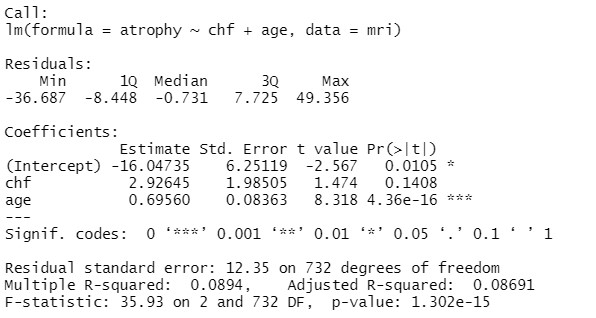
\includegraphics[scale = 0.53]{figures/mri_multiple_eg1}
		
		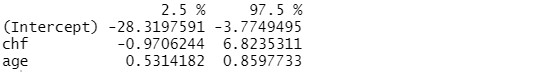
\includegraphics[scale = 0.57]{figures/mri_multiple_cis}
	\end{figure}
	
\end{frame}

\begin{frame}{Interpretation}


We estimate that, comparing groups of Americans over the age of 65 \textcolor{blue}{with the same age}, those with a history of congestive heart failure have an average atrophy score 2.93 points higher than the average atrophy score of those without a history of congestive heart failure.

\bigskip

Based on a 95\% confidence interval, this difference would not be considered unusual if the true difference were between -0.97 and 6.82 points. 

\bigskip

At the 5\% significance level, we fail to reject the null hypothesis that there is no difference in average atrophy score for people \textcolor{blue}{of the same age} with and without congestive heart failure (p = 0.14). 

\bigskip

We conclude that there is not significant evidence of an association between congestive heart failure and atrophy score \textcolor{blue}{when adjusting for age}. 

\end{frame}


\subsection{Causal diagrams}

\begin{frame}{Types of covariates}
Throughout this section, we will consider \textcolor{blue}{three} types of covariates that we may include in our multiple regression models:

\vspace{0.3cm}

\begin{enumerate}
	\item Confounders
	\item Effect modifiers
	\item Precision variables
\end{enumerate}

\vspace{0.3cm}

For each, we'll discuss their need for inclusion in a statistical model based on study design and scientific question. But first, we'll talk about \textcolor{blue}{causal diagrams}, which are a useful tool to help us visualize the potential relationships between variables.

\end{frame}

\begin{frame}{Causal diagrams: Terminology}
Often, when thinking about the need to adjust for additional covariates in a model, it is helpful to draw a \textcolor{blue}{causal diagram} relating the predictor of interest, outcome, and additional covariates. Causal diagrams consist of\dots

\vspace{0.3cm}

\begin{itemize}
	\item \textcolor{blue}{Nodes}: variables (including the predictor of interest, outcome, and additional covariates) \pause
	\medskip
	
	\item \textcolor{blue}{Edges}: connections between nodes, to denote causal relationships or associations \pause
	\medskip
	
	\begin{itemize}
		\item Line: denotes that two variables are associated with one another
		\medskip
		
		\item Arrow: denotes that one variable is \textit{causally related to} another
	\end{itemize} \pause
\medskip
\item \textcolor{blue}{Causal pathway}: a path between nodes in a causal diagram, directed using arrows
\end{itemize}
\end{frame}

\begin{frame}{Causal diagram: Example}
	\begin{figure}
		\centering
		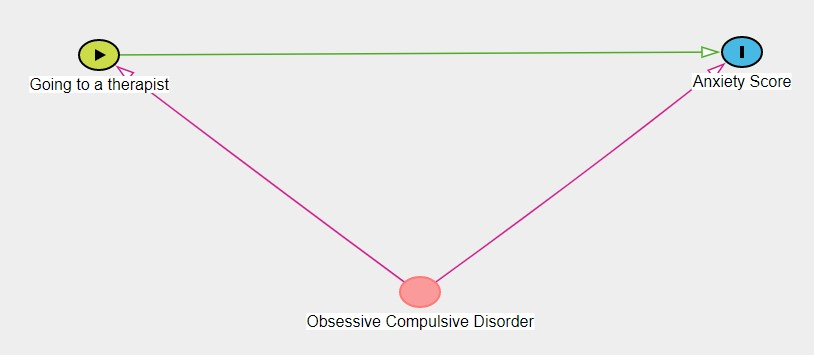
\includegraphics[scale = 0.45]{figures/therapy_dag}
	\end{figure}
\end{frame}

\begin{frame}{Causal diagram: Another Example}
Below is a more complicated example of a causal diagram, with nodes A through H:

\vspace{0.1cm}
\begin{figure}
	\centering 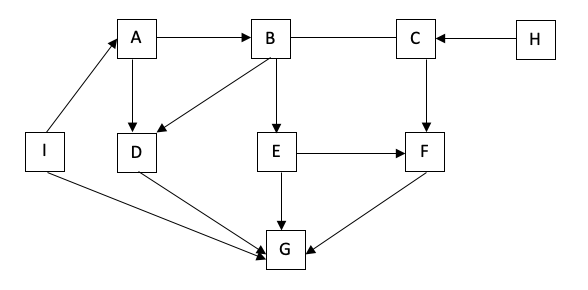
\includegraphics[scale=0.4]{figures/dag1.png}
\end{figure}

\end{frame}

\begin{frame}{Causal diagram: Another Example}

\vspace{-5 mm}

\begin{figure}
	\centering 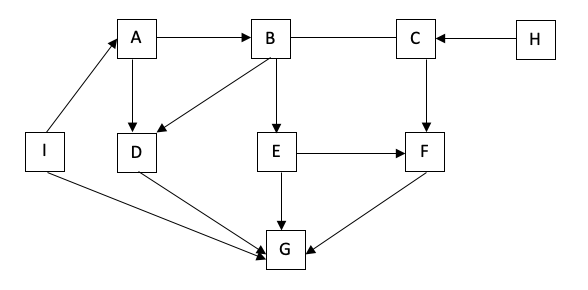
\includegraphics[scale=0.4]{figures/dag1.png}
\end{figure}

\vspace{0.1cm} 

\textcolor{violet}{Pollev}: Which nodes (if any) are on a causal pathway from B to G? It may be useful to list the causal pathways first. 
{\scriptsize \url{https://PollEv.com/multiple_choice_polls/uXSqGzk3gwedQRItnMTtg/respond}}

\end{frame}

\begin{frame}{Causal Diagram Activity}
	In groups, look at the MRI documentation and draw a causal diagram between the general health, physical activity, pack years of smoking, and atrophy variables. 
\end{frame}

%\subsection{Confounders}
%
%% definition slide and example of diagram
%\begin{frame}{Confounders}
%Causal diagrams are useful tools we can use to determine whether or not variables are confounders.
%
%\vspace{0.3cm}
%
%\textcolor{blue}{Confounder} (or ``confounding variable"): is a variable that is \textcolor{blue}{associated with our outcome} and
%also \textcolor{blue}{associated with the exposure} in our sample, which, when we don't adjust for it, creates bias in estimating the effect of the
%exposure on the outcome.
%
%\vspace{0.3cm} \pause
%
%In a causal diagram, confounders look like \dots
%
%\vspace{0.3cm}
%
%\centering 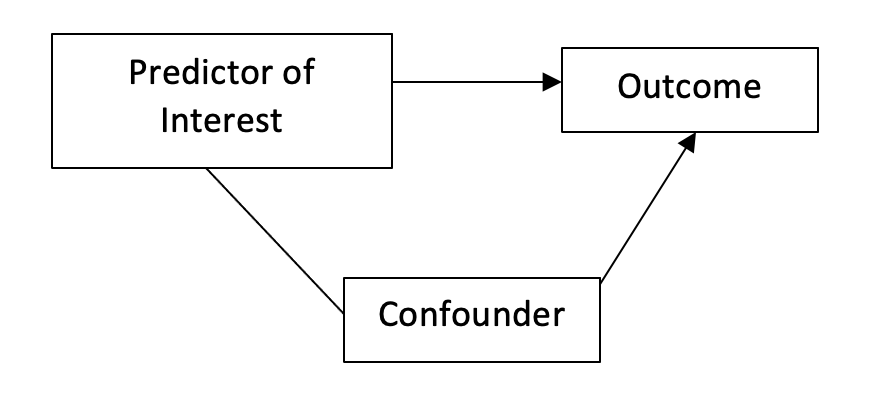
\includegraphics[scale=0.4]{figures/confounder1.png}
%
%\end{frame}
%
%% second diagram example
%\begin{frame}{Confounders}
%Causal diagrams are useful tools we can use to determine whether or not variables are confounders.
%
%\vspace{0.3cm}
%
%\textcolor{blue}{Confounder} (or ``confounding variable"): a variable that is \textit{causally related to} our outcome, and also \textit{associated with} the exposure in our sample
%
%\vspace{0.3cm} 
%
%\dots confounders can also look like this\dots
%
%\vspace{0.3cm}
%
%\centering 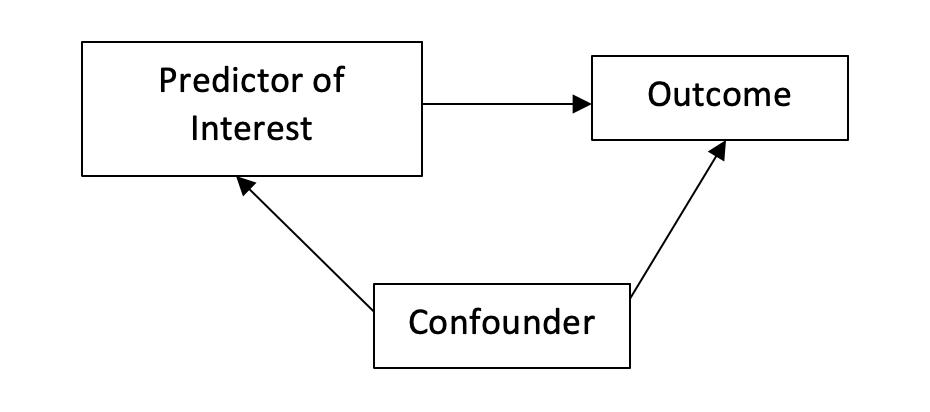
\includegraphics[scale=0.4]{figures/confounder2.png}
%\end{frame}
%
%\begin{frame}{Confounders}
%\vspace{-0.3cm}
%Causal diagrams are useful tools we can use to determine whether or not variables are confounders.
%
%\vspace{0.3cm}
%
%\textcolor{blue}{Confounder} (or ``confounding variable"): a variable that is \textit{causally related to} our outcome, and also \textit{associated with} the exposure in our sample
%
%\vspace{0.3cm} 
%
%\dots but confounders \textcolor{red}{cannot} look like this:
%
%\vspace{0.2cm}
%
%\begin{figure}
%	\centering 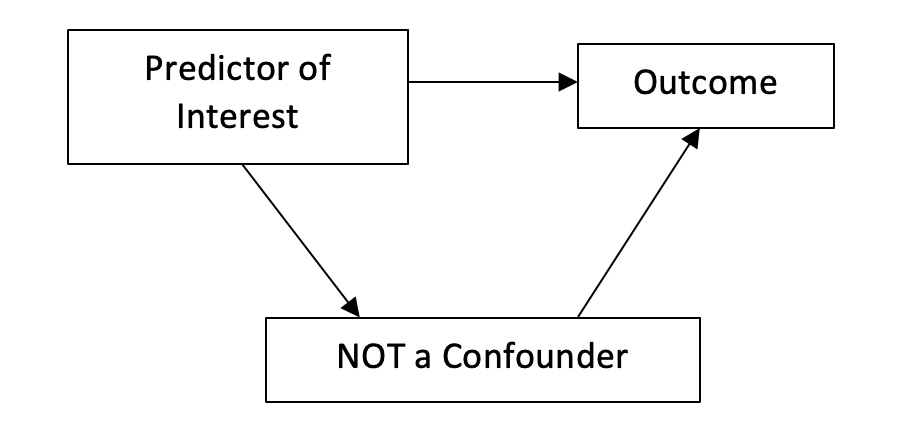
\includegraphics[scale=0.4]{figures/confounder3.png}
%\end{figure}
%
%\vspace{-0.1cm}
%\small Confounder cannot be on the causal pathway from the predictor of interest to the outcome!
%
%\end{frame}
%
%% Example of what to look for graphically
%\begin{frame}{Confounders: what to look for in a graph}
%If your predictor of interest and outcome are both quantitative, and your potential confounder is \textit{binary}, there are some things you can look for in a graph that may indicate whether or not the potential confounder is in fact a confounding variable. \pause
%
%\vspace{0.3cm}
%
%Below we plot an exposure vs. an outcome:
%
%\vspace{0.3cm}
%
%\centering 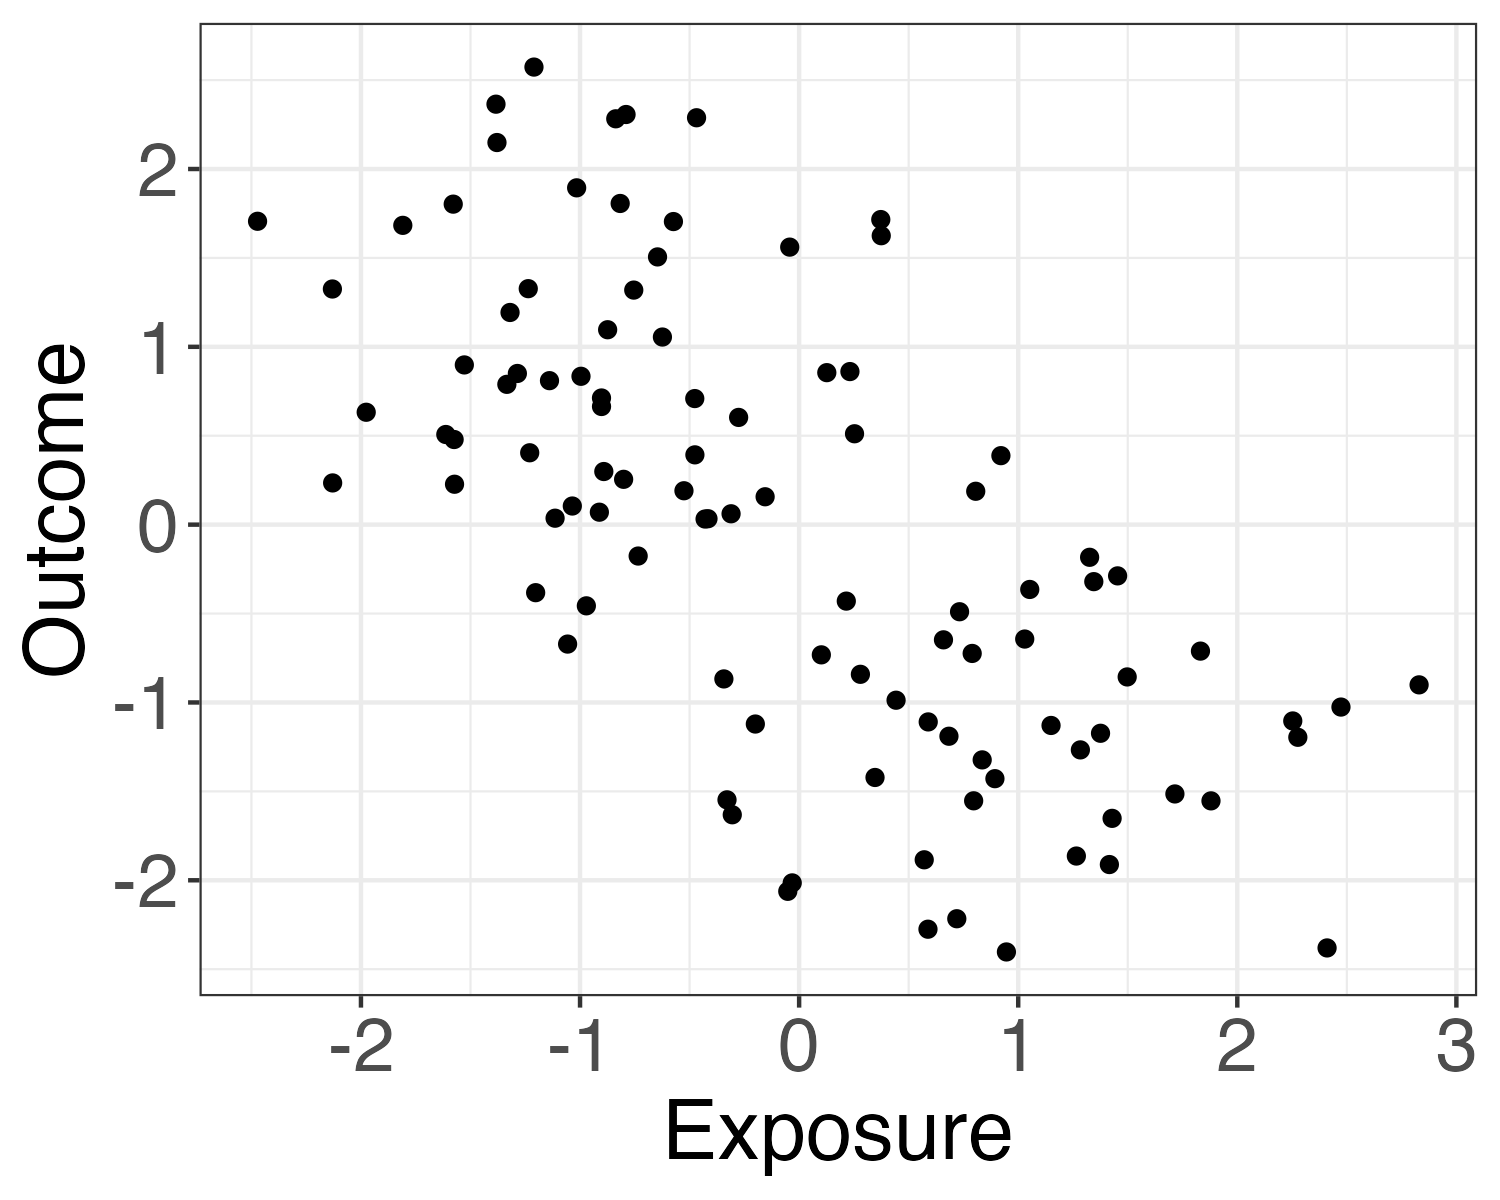
\includegraphics[scale=0.4]{figures/p0.png}
%\end{frame}
%
%\begin{frame}{Confounders: what to look for in a graph}
%We now color the points by our potential confounding variable.
%\vspace{0.3cm}
%
%\begin{figure}
%	\centering 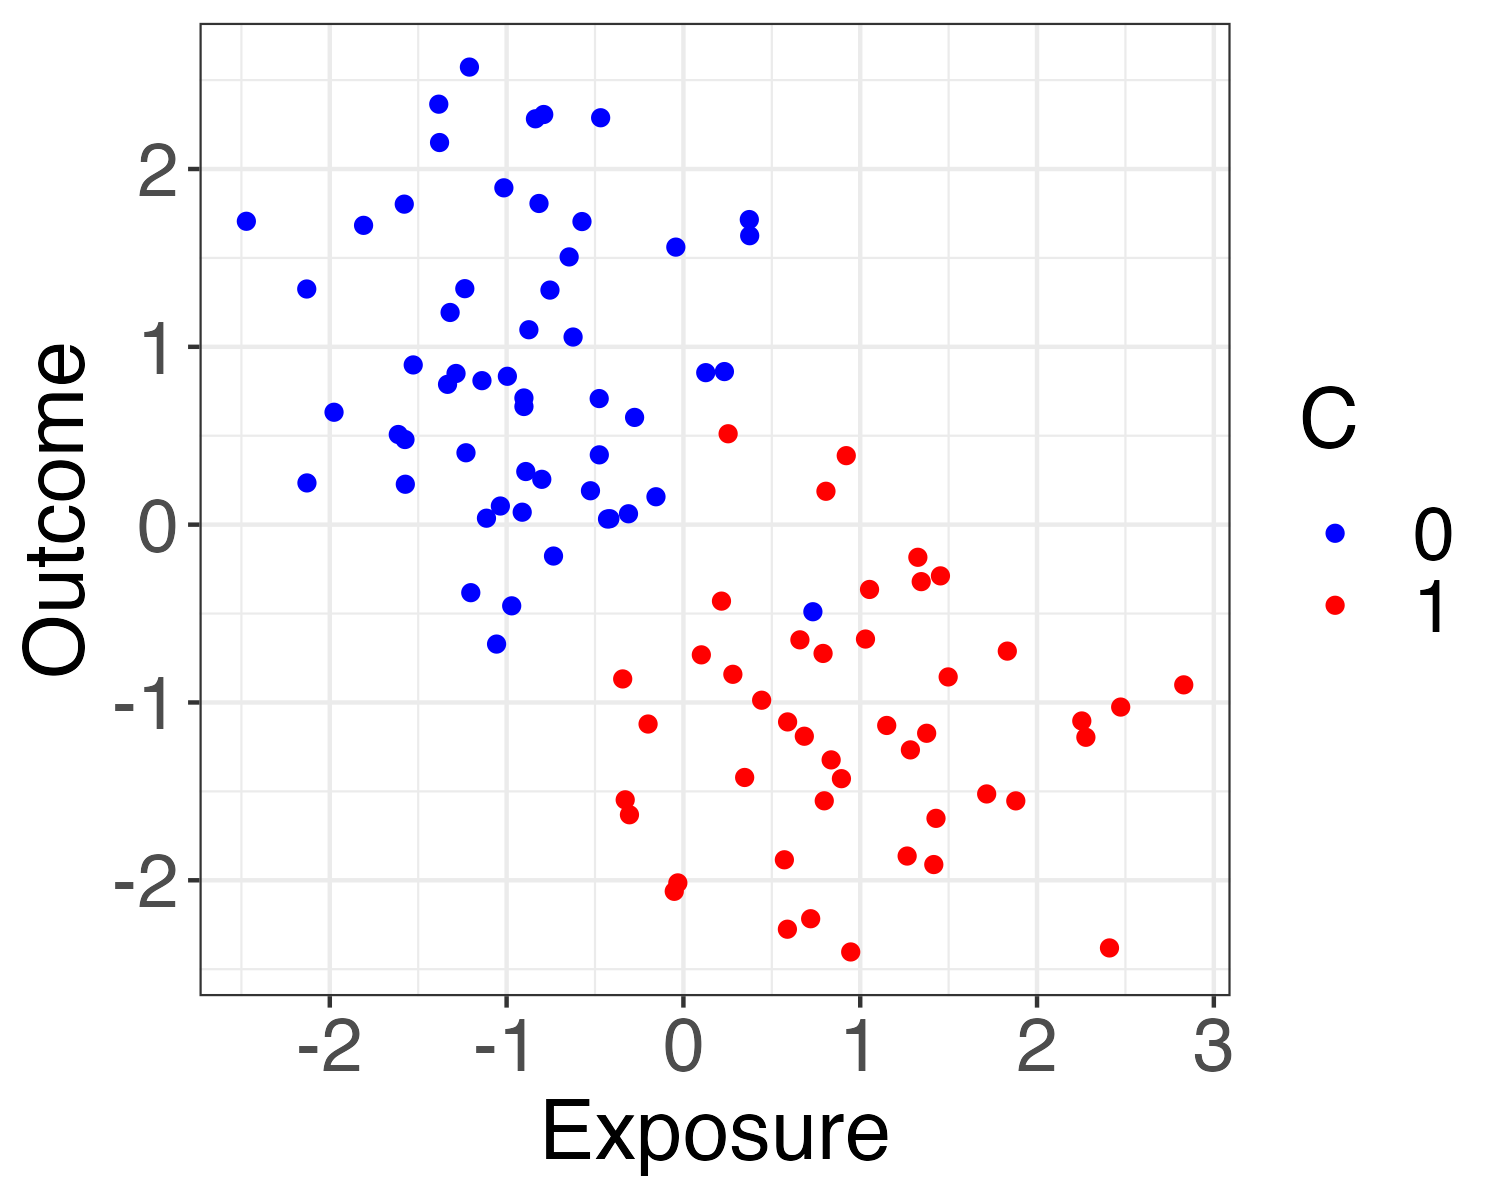
\includegraphics[scale=0.4]{figures/p1.png}
%\end{figure}
%
%\vspace{0.1cm} \pause
%\small We can see from the plot that the potential confounder seems to be associated with exposure (predictor of interest) \textit{in the sample} (one of the requirements for a confounding variable!). The red dots are associated with larger values of exposure, and blue dots with smaller values of exposure. 
%
%\end{frame}
%
%\begin{frame}{Confounders: what to look for in a graph}
%
%\textcolor{red}{Important note}: A graph alone is not enough to determine if a variable is a confounder! You still need to think about whether that variable causes the outcome in the population, which cannot be determined graphically but must be thought about \textit{scientifically}.
%
%\end{frame}
%
%% Example with a question and answer - could be from the worksheet
%\begin{frame}{Confounders: Example}
%\vspace{-0.6cm}
%\textcolor{blue}{Question}: Your friend shows you the following graph\dots
%
%\vspace{0.1cm}
%
%\begin{figure}
%	\centering 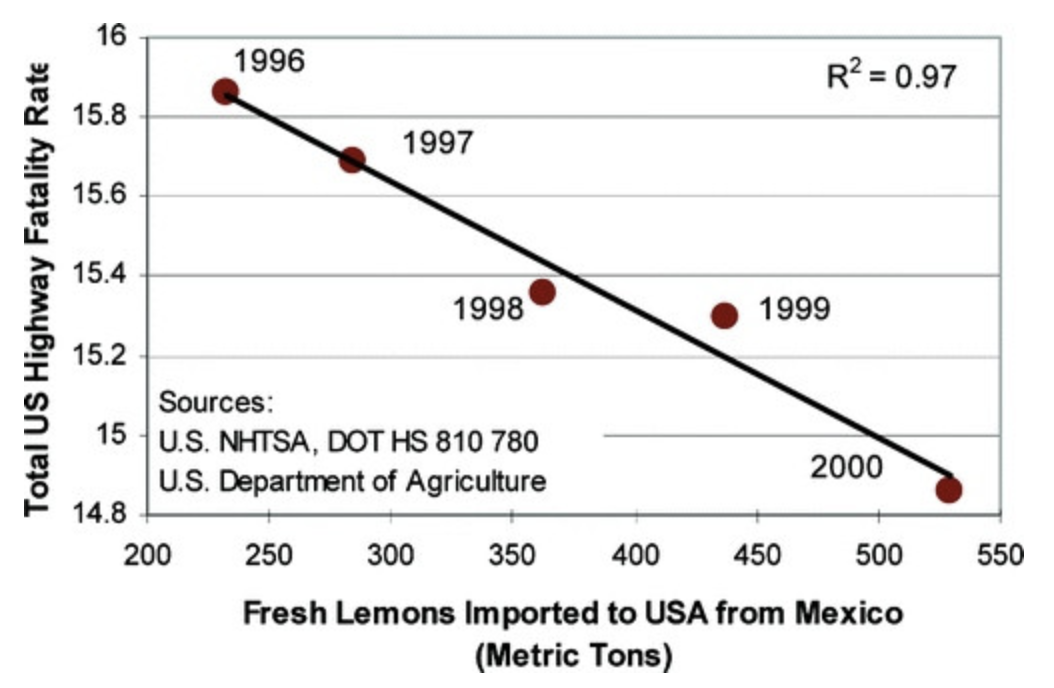
\includegraphics[scale=0.4]{figures/lemons.png}
%\end{figure}
%
%\vspace{0.1cm} 
%
%\dots and says ``More lemons imported from Mexico lead to lower highway fatality rates! We should import more lemons to lower the higher fatality rate!"
%
%
%
%\end{frame}
%
%\begin{frame}{Confounders: Example}
%	\vspace{-0.6cm}
%\begin{figure}
%	\centering 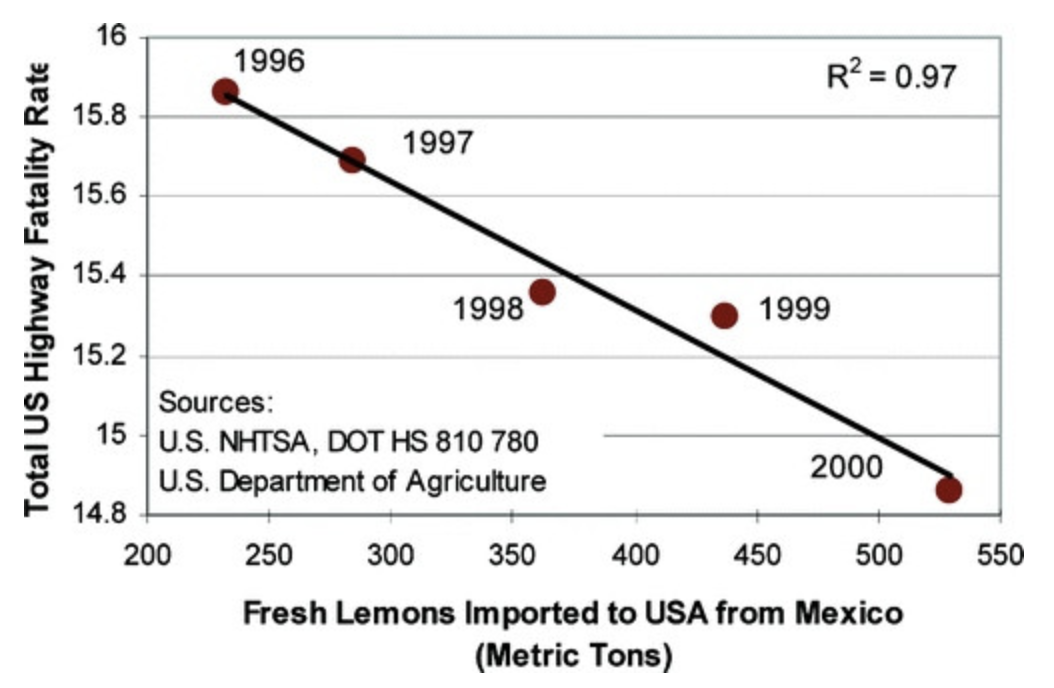
\includegraphics[scale=0.3]{figures/lemons.png}
%\end{figure}
%
%\vspace{0.1cm} 
%
%\dots and says ``More lemons imported from Mexico lead to lower highway fatality rates! We should import more lemons to lower the higher fatality rate!"
%
%\vspace{0.3cm}
%
%You think your friend is being mislead. What confounding variable is at play here, and what other possible explanation could there be for this observed relationship?
%\end{frame}
%
%\begin{frame}{Confounders: Example}
%\textcolor{blue}{Question}: You think your friend is being mislead. What confounding variable is at play here, and what other possible explanation could there be for this observed relationship?
%
%\vspace{0.3cm}
%
%\textcolor{blue}{Answer}: From the graph, we can see that highway fatality rates have decreased \textit{over time}, and number of lemons imported has increased \textit{over time}. Time is a confounding variable in this case. Highway fatality rates have likely decreased over time because cars have gotten much safer with improved airbag quality and other innovations. Number of fresh lemons imported has increased over time, potentially because the US population has increased (and therefore demands more lemons).
%\end{frame}
%
%
%\begin{frame}{Confounders and study design}
%	\vspace{-0.3cm}
%When our scientific question involves a causal relationship, whether or not we \textit{need} to adjust for covariates depends on the study design.
%
%\vspace{0.3cm}
%
%When reviewing study design, we said that a randomized controlled trial is the only study design in which we can confidently make causal claims about relationships between variables. \textit{However}, if we are able to adjust for \textit{all possible confounders} in an observational study, we could also make causal statements for these study designs. In practice, situations where we can confidently say we've adjusted for all possible confounders are extremely rare. Nevertheless, it is good to adjust for any possible confounders we have, so long as we are still answering a scientific question of interest. \pause
%
%\vspace{0.3cm}
%
%\begin{itemize}
%	\item \textcolor{blue}{Randomized controlled trial:} no need to adjust because there are no possible confounders (unless randomization has failed)
%	\item \textcolor{blue}{Observational study:} must adjust for all possible confounders in order to make causal claims, should adjust for all potential confounders regardless
%\end{itemize}
%\end{frame}
%
%\begin{frame}{Confounders: regression equation}
%Writing regression equations including confounding variables is as simple as adding in an additional covariate. Suppose
%
%\vspace{0.3cm}
%
%\begin{itemize}
%	\item $Y$ = outcome
%	\item $X$ = predictor of interest
%	\item $Z$ = confounder
%\end{itemize}
%
%\vspace{0.3cm}
%
%Then to include the confounding variable $Z$ into our model, we would write
%$$
%E[Y \mid X, Z] = \beta_0 + \beta_1 X + \beta_2 Z
%$$
%
%If we instead had \textit{two} confounding variables $Z$ and $W$, we would write
%$$
%E[Y \mid X, Z, W] = \beta_0 + \beta_1 X + \beta_2 Z + \beta_3 W
%$$
%\dots and so forth with additional confounding variables!
%
%\end{frame}
%
%\begin{frame}{Confounders: Example in \texttt{R}}
%Thinking back to our \texttt{births} dataset, we are interested in the association between First Steps participation and birthweight. Since this is an observational study, confounding is a potential concern. In particular, we think that age may be a confounding variable, since 
%
%\vspace{0.3cm}
%
%\begin{itemize}
%	\item Age is associated with First Steps participation in the sample
%	\item Giving birth at a young age may increase the risk of birth complications, leading to low birthweights (a causal relationship)
%\end{itemize} 
%
%\begin{figure}
%	\centering 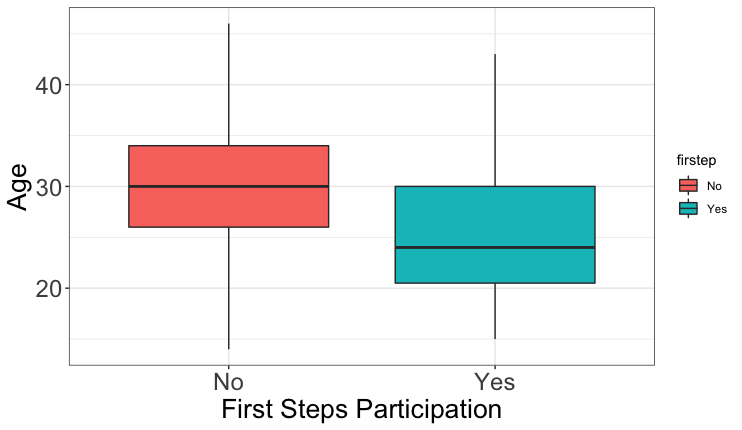
\includegraphics[scale=0.2]{figures/age_firstep.png}
%\end{figure}
%
%\end{frame}
%
%\begin{frame}{Confounders: Example in \texttt{R}}
%Thinking back to our \texttt{births} dataset, we are interested in the association between First Steps participation and birthweight. Since this is an observational study, confounding is a potential concern. In particular, we think that age may be a confounding variable, since 
%
%\vspace{0.3cm}
%
%\begin{itemize}
%	\item Age is associated with First Steps participation in the sample
%	\item Giving birth at a young age may increase the risk of birth complications, leading to low birthweights (a causal relationship)
%\end{itemize} 
%
%\vspace{0.3cm}
%
%We can write our regression model as
%$$
%E[\texttt{bwt} \mid \texttt{FS}, \texttt{age}] = \beta_0 + \beta_1 \times \texttt{FS} + \beta_2 \times \texttt{age}
%$$
%\end{frame}
%
%\begin{frame}{Confounders: Example in \texttt{R}}
%Fitting this model in \texttt{R} is similar to simple linear regression models, we just need to add our additional variable to the formula argument as follows:
%
%\vspace{0.3cm}
%
%\centering 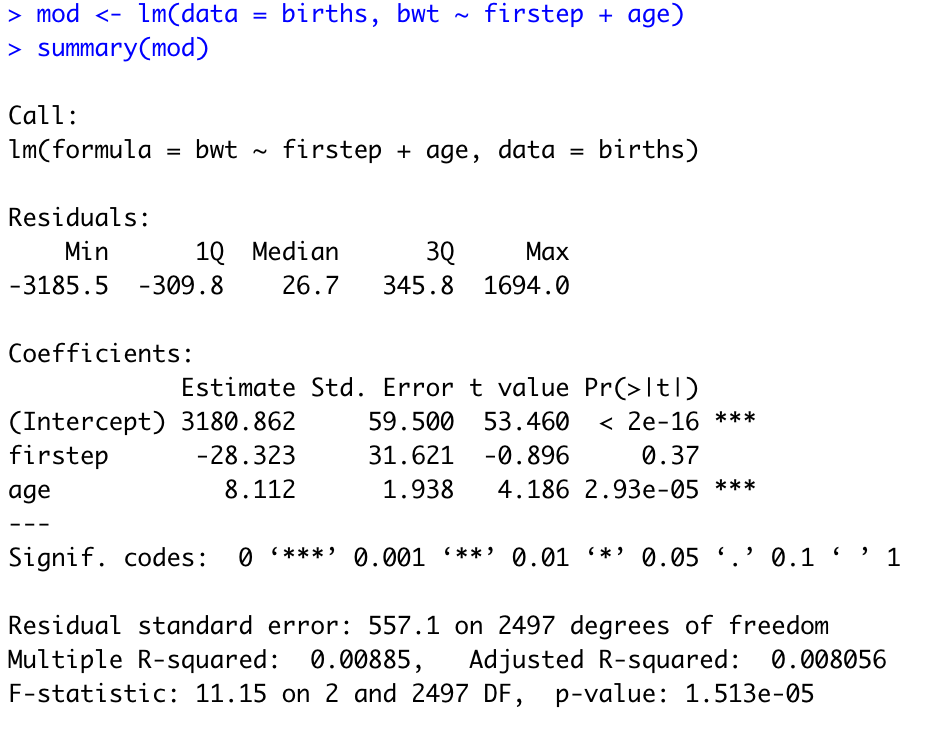
\includegraphics[scale=0.4]{figures/confound_code.png}
%\end{frame}
%
%\begin{frame}{Confounders: Example in \texttt{R}}
%Fitting this model in \texttt{R} is similar to simple linear regression models, we just need to add our additional variable to the formula argument as follows:
%
%\vspace{0.3cm}
%
%\centering 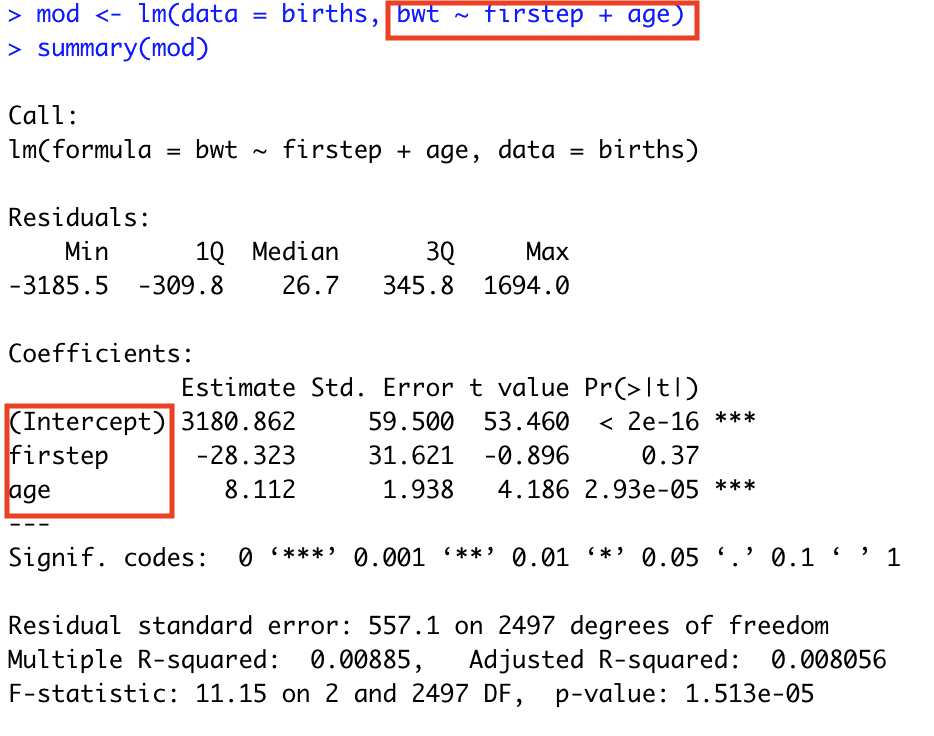
\includegraphics[scale=0.4]{figures/confound_code2.png}
%\end{frame}
%
%\begin{frame}{Confounders: Example in \texttt{R}}
%From our multiple regression output, we have coefficient estimates and standard errors for each variable in our model:
%
%\vspace{0.3cm}
%
%\begin{itemize}
%	\item $\beta_0$: 3180.862 (SE = 59.5)
%	\item $\beta_1$ (Coefficient for FS): -28.323 (SE = 31.62)
%	\item $\beta_2$ (Coefficient for age): 8.112 (SE = 1.94)
%\end{itemize}
%
%\vspace{0.3cm}
%	
%(remember that if we want confidence intervals for our estimates we can either use the \texttt{confint} function on our model, or we can compute them by hand using the standard errors above)
%
%\vspace{0.3cm}
%
%\textcolor{blue}{Question}: How do we interpret the results of our regression model, in the context of our scientific question?
%
%	
%\end{frame}
%
%\begin{frame}{Confounders: Example in \texttt{R}}
%\textcolor{blue}{Question}: How do we interpret the results of our regression model, in the context of our scientific question?
%
%\vspace{0.3cm}
%
%\textcolor{blue}{Answer}: The association we are interested in is between First Steps participation and birthweight, with age as a confounding variable. The coefficient that corresponds to the association between FS and birthweight is $\beta_1$.
%
%\vspace{0.3cm}
%
%\textcolor{cyan}{We estimate that average birthweight is 28.3 grams higher for birth parents who did not participate in FS compared to those who did, for birth parents of the same age. This observed difference would not be surprising if the true difference in average birthweight were between -90.3 grams and  33.7 grams.} \pause
%
%\vspace{0.3cm}
%
%*We could of course interpret $\beta_0$ and $\beta_2$ in this model as well, but $\beta_1$ is the coefficient that corresponds to our scientific question!
%\end{frame}



%\subsection{Effect modifiers}
%
%% definition slide and example of diagram
%\begin{frame}{Effect modifiers}
%Causal diagrams are \textit{also} useful tools we can use to determine whether or not variables are effect modifiers.
%
%\vspace{0.3cm}
%
%\textcolor{blue}{Effect modifiers}: a variable that modifies the association between the predictor of interest and the outcome. In other words, the association between the predictor of interest and the outcome \textit{depends on} the effect modifier. \pause
%
%\vspace{0.3cm}
%
%In a causal diagram, we denote effect modifiers like this:
%
%\vspace{0.1cm}
%
%\begin{figure}
%	\centering 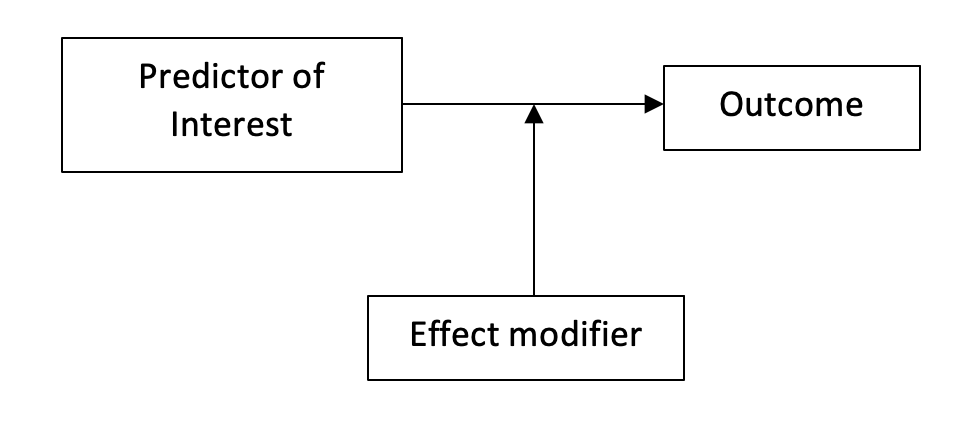
\includegraphics[scale=0.4]{figures/effectmod1.png}
%\end{figure}
%\end{frame}
%
%
%% Example of what to look for graphically
%\begin{frame}{Effect modifiers: what to look for in a graph}
%If your predictor of interest and outcome are both quantitative, and your potential effect modifier is \textit{binary}, there are some things you can look for in a graph that may indicate whether or not the potential effect modifier is in fact an effect modifier. \pause
%
%\vspace{0.3cm}
%
%Below we plot an exposure vs. an outcome:
%
%\vspace{0.3cm}
%
%\centering 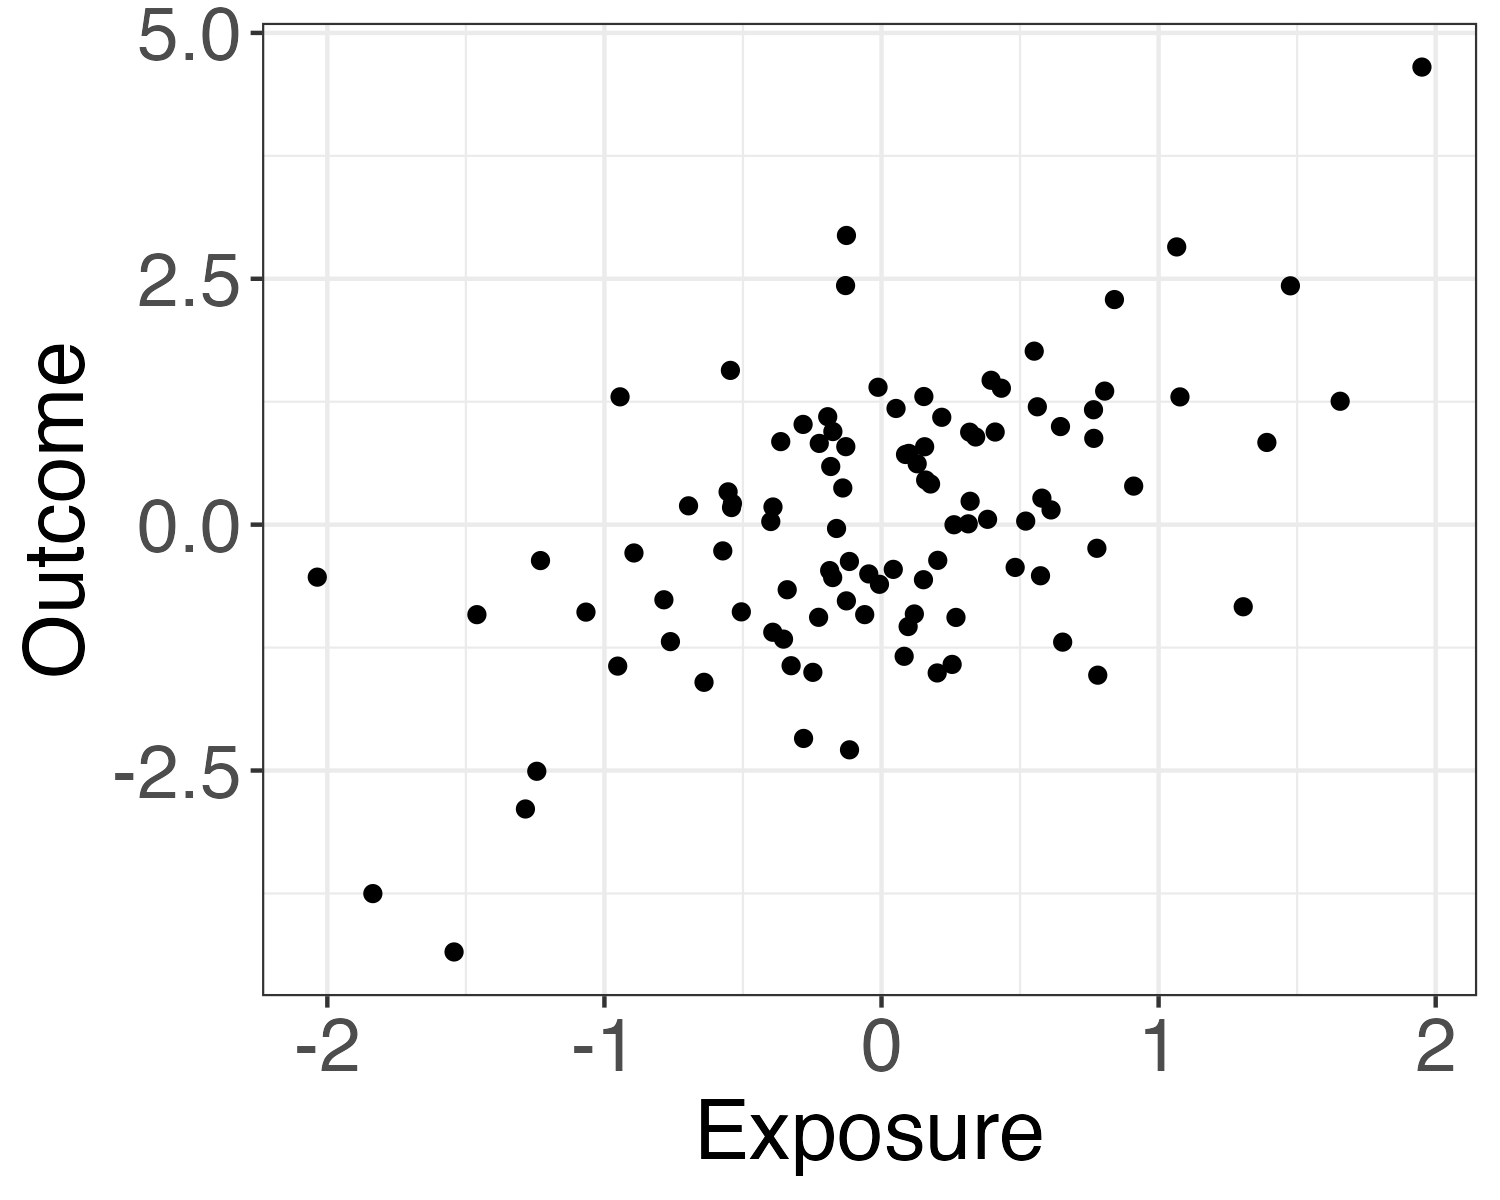
\includegraphics[scale=0.4]{figures/p2.png}
%\end{frame}
%
%\begin{frame}{Effect modifiers: what to look for in a graph}
%We now color the points by our potential effect modifier\dots
%\vspace{0.3cm}
%
%\begin{figure}
%	\centering 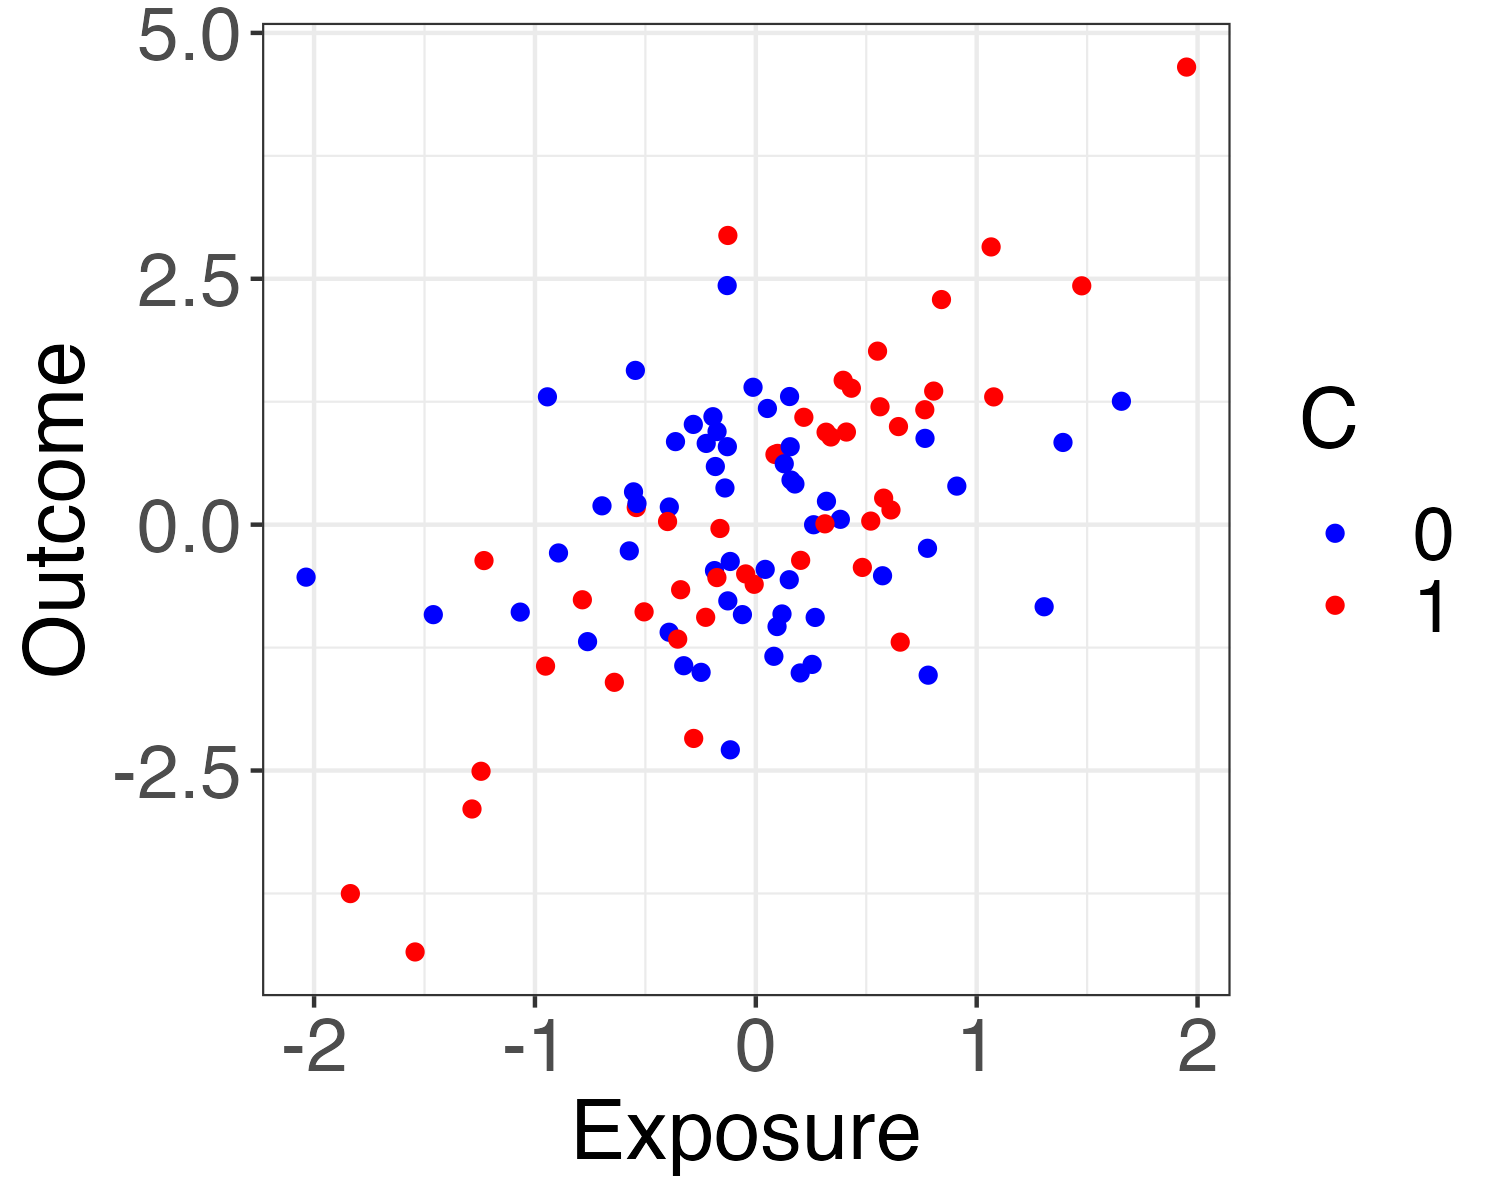
\includegraphics[scale=0.4]{figures/p3.png}
%\end{figure}
%
%\end{frame}
%
%\begin{frame}{Effect modifiers: what to look for in a graph}
%\dots and if we were to fit simple linear regressions for each group defined by our potential effect modifier (a stratified analysis), we could add those regression lines to the plot as well:
%
%\vspace{0.3cm}
%
%\begin{figure}
%	\centering 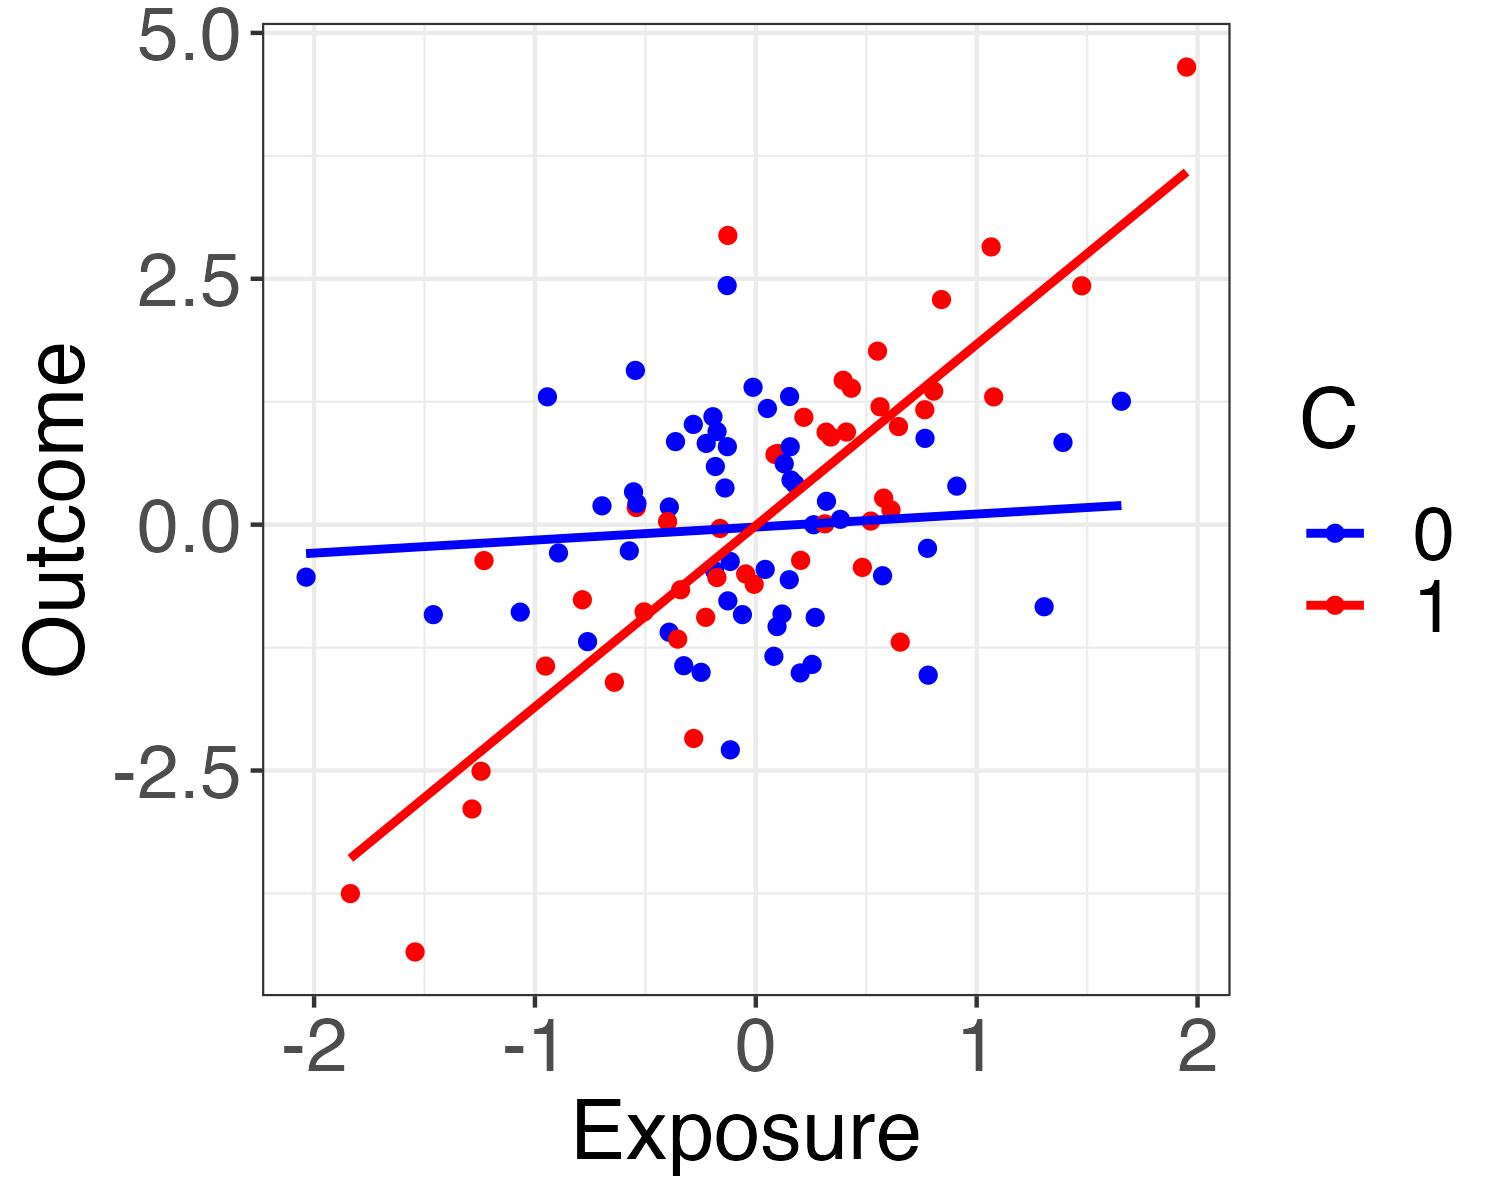
\includegraphics[scale=0.4]{figures/p4.png}
%\end{figure}
%
%\end{frame}
%
%\begin{frame}{Effect modifiers: what to look for in a graph}
%
%\begin{figure}
%	\centering 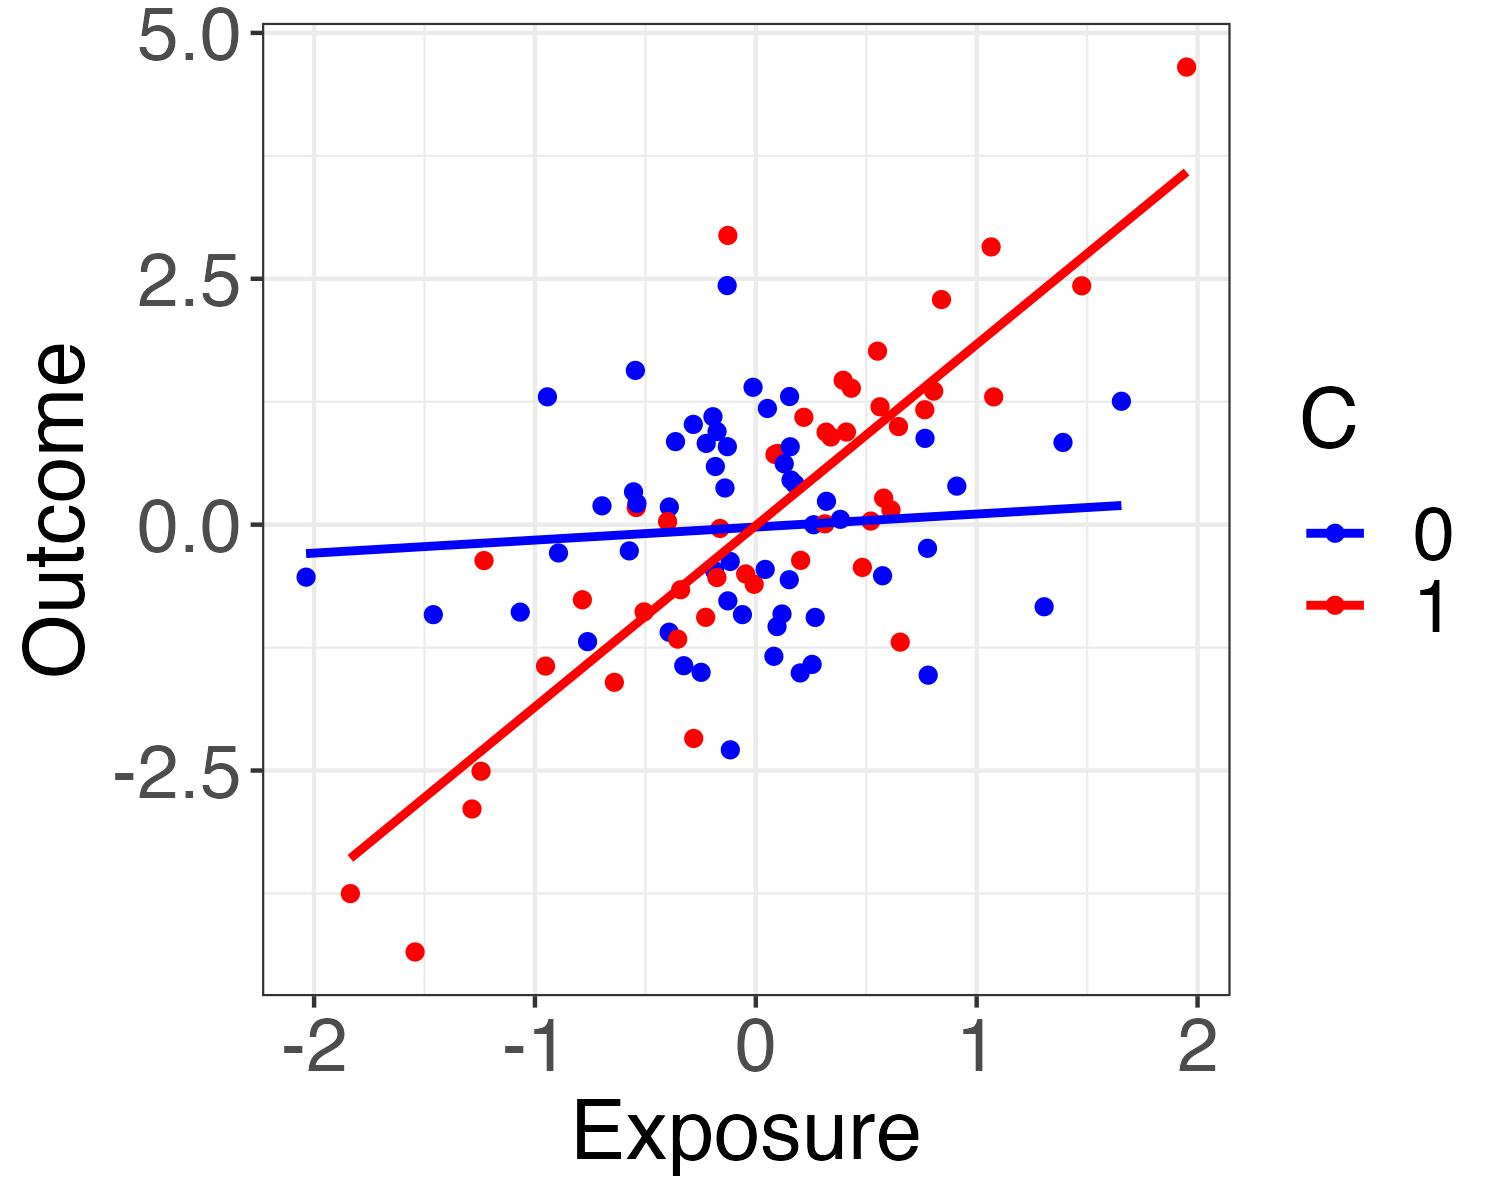
\includegraphics[scale=0.4]{figures/p4.png}
%\end{figure}
%
%\vspace{0.3cm}
%
%The key thing to note here is that groups defined by a binary effect modifier will have linear regression lines with different \textcolor{blue}{slopes} \textit{and} different \textcolor{blue}{intercepts}. This indicates that the association between the exposure and the outcome has been \textit{modified} by the additional variable, and thus the additional variable is an effect modifier.
%
%\end{frame}
%
%\begin{frame}{Effect modifiers: always adjust}
%When our scientific question addresses whether or not the association between a predictor of interest and the outcome differs by an additional covariate (effect modifier), you \textit{must} adjust for the covariate in your model. Otherwise, your model would not adequately answer the scientific question.
%\\ ~\ 
%
%When the scientific question doesn't address the association differing by a potential effect modifier, then you don't necessarily need to include it. 
%
%\vspace{0.3cm}
%
%(Note that this is different from a confounder, where we do not need to adjust for confounding variables in a randomized controlled trial, so long as randomization was successful, but we \textit{must} adjust in an observational study if we want to make causal claims.)
%
%
%\end{frame}
%
%\begin{frame}{Effect modifiers: regression equation}
%The presence of an effect modifier is called an \textcolor{blue}{interaction}, and means we will need to include an interaction \textit{term} in our statistical model. In regression equations, interaction terms are modeled as the \textit{multplication} of the potential effect modifier and the predictor of interest. Suppose
%\vspace{0.3cm}
%
%\begin{itemize}
%	\item $Y$ = outcome
%	\item $X$ = predictor of interest
%	\item $Z$ = potential effect modifier
%\end{itemize}
%
%\vspace{0.3cm}
%
%Then to include the potential effect modifier into our model, we would write,
%$$
%E[Y \mid X, Z] = \beta_0 + \beta_1 X + \beta_2 Z + \beta_3 (X \times Z)
%$$
%\end{frame}
%
%\begin{frame}{Effect modifiers: regression equation}
%\vspace{-0.5cm}
%$$
%E[Y \mid X, Z] = \beta_0 + \beta_1 X + \beta_2 Z + \beta_3 (X \times Z)
%$$
%New terminology:
%\begin{itemize}
%	\item The terms $X$ and $Z$ are called \textcolor{blue}{main effects}
%	\item The multiplicative term $(X \times Z)$ is called the \textcolor{blue}{interaction term}
%\end{itemize}
%
%\vspace{0.3cm}
%
%You must \textcolor{red}{always} include the main effects in your model if you include an interaction term. Not including the main effects changes the interpretation of the interaction term. We'll see an example of interpreting the coefficient for the interaction term in the next few slides\dots
%
%\end{frame}
%
%\begin{frame}{Effect modifiers: Example in \texttt{R}}
%Thinking back to our \texttt{births} dataset, suppose we are interested in whether or not the association between age and birthweight differs for individuals in First Steps vs. those not in First Steps. Since we are interested in how an association between a predictor of interest and outcome varies based on another variable, we are interested in \textcolor{blue}{effect modification}. \pause
%
%\vspace{0.3cm}
%
%We can write our regression model as 
%$$
%E[\texttt{bwt} \mid \texttt{FS}, \texttt{age}] = \beta_0 + \beta_1 \times \texttt{FS} + \beta_2 \times \texttt{age} + \beta_3 \times (\texttt{FS} \times \texttt{age})
%$$
%
%\end{frame}
%
%\begin{frame}{Effect modifiers: Example in \texttt{R}}
%\vspace{-0.4cm}
%Fitting this model in \texttt{R} is similar to multiple linear regression models we've seen, but we now need to include an interaction term in our formula. There are a couple ways to do this:
%
%\vspace{0.3cm}
%
%\begin{enumerate}
%	\item \texttt{lm(dataframe, formula = outcome} $\sim$ \texttt{var1 + var2 + var1:var2)}
%	\item \texttt{lm(dataframe, formula = outcome} $\sim$ \texttt{var1*var2)}
%\end{enumerate}
%
%\vspace{0.3cm}
%
%The first option involves fully writing out the main effects and the interaction term separately, with the interaction term denoted with a ``:" separating the two variables that interact.
%
%\vspace{0.3cm}
%
%The second option involves specifying the interaction term with a ``*" symbol, which tells \texttt{R} to automatically include the main effects for you.
%
%\vspace{0.3cm}
%
%Either option is completely fine to use, and both will give you the same results!
%
%\end{frame}
%
%\begin{frame}{Effect modifiers: Example in \texttt{R}}
%We fit our model for the births dataset in \texttt{R} as follows:
%
%\vspace{0.3cm}
%
%\centering 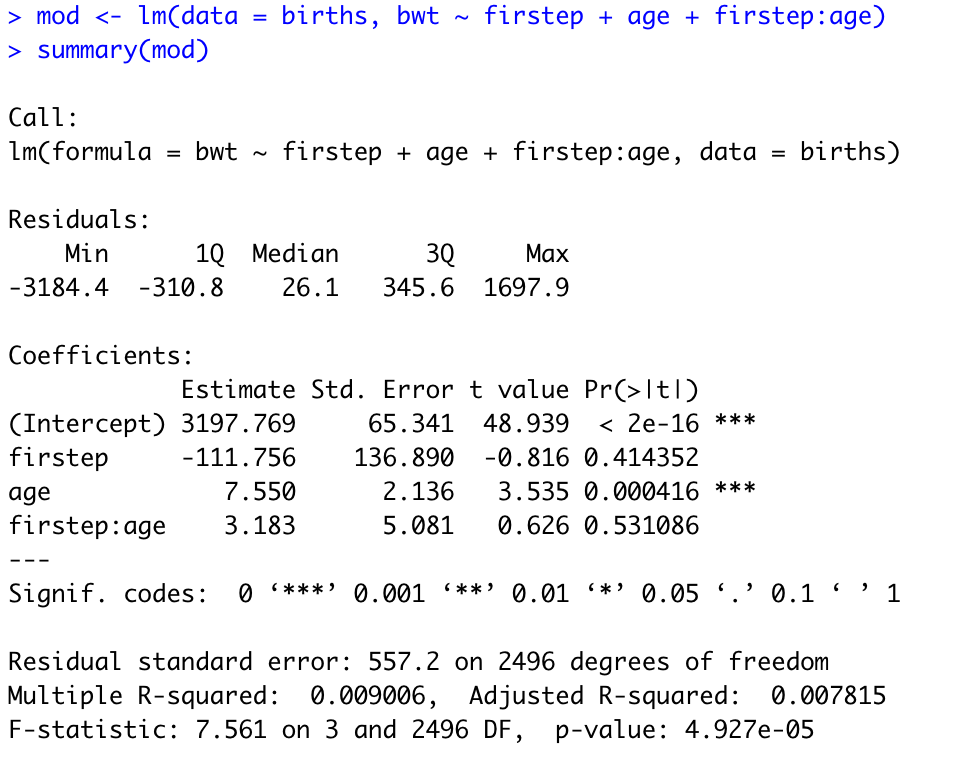
\includegraphics[scale=0.4]{figures/interact_mod.png}
%\end{frame}
%
%\begin{frame}{Effect modifiers: Example in \texttt{R}}
%We fit our model for the births dataset in \texttt{R} as follows:
%
%\vspace{0.3cm}
%
%\centering 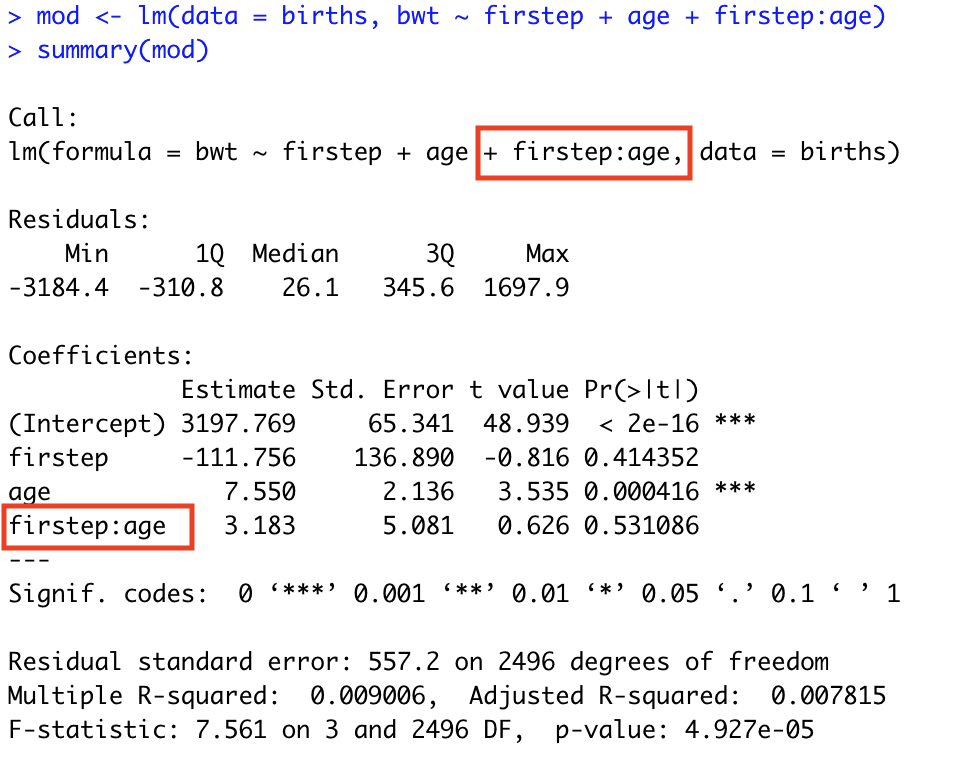
\includegraphics[scale=0.4]{figures/interact_mod2.png}
%\end{frame}
%
%\begin{frame}{Effect modifiers: Example in \texttt{R}}
%From our multiple regression output, we have coefficient estimates and (we can obtain) confidence intervals for each variable in our model:
%
%\vspace{0.3cm}
%
%\begin{itemize}
%	\item $\beta_0$: 3197.8 (3069.6, 3325.9)
%	\item $\beta_1$ (Coefficient for FS): -111.8 (-380.2, 156.7)
%	\item $\beta_2$ (Coefficient for age): 7.6 (3.4, 11.7)
%	\item $\beta_3$ (Coefficient for FS * age): 3.2 (-6.8, 13.1)
%\end{itemize}
%
%\vspace{0.3cm}
%
%
%\textcolor{blue}{Question:} How do we interpret the coefficients in our regression model, in the context of our scientific question? 
%\end{frame}
%
%\begin{frame}{Interpreting interaction terms}
%Thinking back to our regression equation for effect modifiers, we had
%
%$$
%E[Y \mid X, Z] = \beta_0 + \beta_1 X + \beta_2 Z + \beta_3 (X \times Z)
%$$
%
%$\beta_0$: The mean value of $Y$ when both $X$ and $Z$ are 0.
%
%\vspace{0.3cm}
%
%\textcolor{blue}{Why?} \pause $E[Y, X = 0, Z = 0] = \beta_0 + \beta_1 \times 0 + \beta_2 \times 0 + \beta_3 (0 \times 0) = \beta_0$
%
%\pause \vspace{0.3cm}
%
%Note that this is the same interpretation we have for an intercept in a model that does \textit{not} include an interaction term!
%
%\end{frame}
%
%\begin{frame}{Interpreting interaction terms}
%Thinking back to our regression equation for effect modifiers, we had
%
%$$
%E[Y \mid X, Z] = \beta_0 + \beta_1 X + \beta_2 Z + \beta_3 (X \times Z)
%$$
%
%$\beta_1$: The average difference in $Y$ comparing two groups that differ in one unit of $X$, for groups with $Z = 0$.
%
%\vspace{0.3cm}
%
%\textcolor{blue}{Why?} \pause 
%
%\begin{align*}
%E[Y & \mid X = x + 1, Z = 0] - E[Y  \mid X = x, Z = 0] \\
%& = [\beta_0 + \beta_1 (x +1) + \beta_2 (0) + \beta_3 (x + 1)(0)] \\
%& \hspace{0.3cm}- [\beta_0 + \beta_1 x + \beta_2 (0) + \beta_3 (x)(0)] \\
%& = [\beta_0 + \beta_1 x + \beta_1] - [\beta_0 + \beta_1 x] \\
%& = \beta_1
%\end{align*}
%
%\end{frame}
%
%\begin{frame}{Interpreting interaction terms}
%Thinking back to our regression equation for effect modifiers, we had
%
%$$
%E[Y \mid X, Z] = \beta_0 + \beta_1 X + \beta_2 Z + \beta_3 (X \times Z)
%$$
%
%$\beta_2$: The average difference in $Y$ comparing two groups that differ in one unit of $Z$, for groups with $X= 0$.
%
%\vspace{0.3cm}
%
%\textcolor{blue}{Why?} \pause 
%
%\begin{align*}
%E[Y & \mid X = 0, Z = z + 1] - E[Y  \mid X = 0, Z = z] \\
%& = [\beta_0 + \beta_1 (0) + \beta_2 (z + 1) + \beta_3 (0)(z + 1)] \\
%& \hspace{0.3cm}- [\beta_0 + \beta_1 (0) + \beta_2 z + \beta_3 (0)(z)] \\
%& = [\beta_0 + \beta_2 z + \beta_2] - [\beta_0 + \beta_2 z] \\
%& = \beta_2
%\end{align*}
%\end{frame}
%
%\begin{frame}{Interpreting interaction terms}
%Thinking back to our regression equation for effect modifiers, we had
%
%$$
%E[Y \mid X, Z] = \beta_0 + \beta_1 X + \beta_2 Z + \beta_3 (X \times Z)
%$$
%
%$\beta_3$: The \textit{difference} in average differences in $Y$ comparing two groups that differ in one unit of $X$, for groups that differ by one unit of $Z$ 
%
%\vspace{0.3cm}
%
%OR: The \textit{difference} in average differences in $Y$ comparing two groups that differ in one unit of $Z$, for groups that differ by one unit of $X$
%
%
%\end{frame}
%
%\begin{frame}{Interpreting interaction terms}
%Thinking back to our regression equation for effect modifiers, we had
%
%$$
%E[Y \mid X, Z] = \beta_0 + \beta_1 X + \beta_2 Z + \beta_3 (X \times Z)
%$$
%
%$\beta_3$: The difference in [average differences in $Y$ comparing two groups that differ in one unit of $X$], for groups that differ by one unit of $Z$ 
%
%\vspace{0.3cm}
%
%OR: The difference in [average differences in $Y$ comparing two groups that differ in one unit of $Z$], for groups that differ by one unit of $X$
%
%\vspace{0.3cm}
%\pause
%The interpretation of the interaction term is a mouthful, but it is correct. \textcolor{blue}{When in doubt, borrow the example interpretation in a few slides and replace with your variables.}
%
%\vspace{0.3cm}
%
%\end{frame}
%
%\begin{frame}{Interaction terms and hypothesis tests}
%When testing whether or not effect modification has occurred, the coefficient corresponding to the interaction term (in the last example, $\beta_3$) is the one we are interested in. 
%
%\vspace{0.3cm}
%
%For the model
%$$
%E[Y \mid X, Z] = \beta_0 + \beta_1 X + \beta_2 Z + \beta_3 (X \times Z)
%$$
%our null and alternative hypotheses for testing for effect modification are:
%
%\vspace{0.3cm}
%
%\begin{itemize}
%	\item $H_0: \beta_3 = 0$
%	\item $H_1: \beta_3 \neq 0$
%\end{itemize}
%
%\end{frame}
%
%\begin{frame}{Effect modifiers: Example in \texttt{R}}
%Back to our example from the births dataset:
%
%\vspace{0.3cm}
%
%\begin{itemize}
%	\item $\beta_0$: 3197.8 (3069.6, 3325.9)
%	\item $\beta_1$ (Coefficient for FS): -111.8 (-380.2, 156.7)
%	\item $\beta_2$ (Coefficient for age): 7.6 (3.4, 11.7)
%	\item $\beta_3$ (Coefficient for FS * age): 3.2 (-6.8, 13.1)
%\end{itemize}
%
%\vspace{0.3cm}
%
%
%\textcolor{blue}{Question:} How do we interpret the coefficients in our regression model, in the context of our scientific question? 
%\end{frame}
%
%\begin{frame}{Effect modifiers: Example in \texttt{R}}
%\textcolor{blue}{Question:} How do we interpret the coefficients in our regression model, in the context of our scientific question? 
%
%\vspace{0.3cm}
%
%\textcolor{blue}{Answer:} Since one of the variables in our interaction term is binary (First Steps participation), the interpretation of the interaction term is more straightforward since groups that differ by one unit in First Steps are just those who participated vs. those who did not.
%
%\vspace{0.3cm}
%
%\textcolor{cyan}{Among those who did not participate in FS, we estimate that the average birthweight is 7.6 grams higher for birth parents differing by 1 year in age, with the older group having higher birthweights. Among those who did participate in FS, we estimate that the average birthweight is 10.8 grams higher for birth parents differing by 1 year in age, with the older group having higher birthweights. The observed difference in association between age and birthweight comparing those in FS and those not would not be surprising if the true difference were between -6.8 and 13.1 grams (p = 0.53).}
%
%\end{frame}
%
%\begin{frame}{Effect modifiers: Example in \texttt{R}}
%\textcolor{cyan}{Among those who did not participate in FS, we estimate that the average birthweight is 7.6 grams higher for birth parents differing by 1 year in age, with the older group having higher birthweights. Among those who did participate in FS, we estimate that the average birthweight is 10.8 grams higher for birth parents differing by 1 year in age, with the older group having higher birthweights. The observed difference in association between age and birthweight comparing those in FS and those not would not be surprising if the true difference were between -6.8 and 13.1 grams (p = 0.53).}
%
%\vspace{0.3cm}
%
%How did we get 7.6 and 10.8?
%\end{frame}
%
%\begin{frame}{Effect modifiers: Example in \texttt{R}}
%	\vspace{-0.4cm}
%How did we get 7.6 and 10.8?
%
%\vspace{0.3cm} If we substitute our estimated coefficients into our regression model statement, we have
%$$
%E[\texttt{bwt} \mid \texttt{FS}, \texttt{age}] = 3197.8 - 111.8 \texttt{FS} + 7.6 \texttt{age} + 3.2 (\texttt{FS} \times \texttt{age}) 
%$$
%\pause Then when $\texttt{FS} = 1$, our regression equation becomes
%\begin{align*}
%E[\texttt{bwt} \mid \texttt{FS} = 1, \texttt{age}] & = 3197.8 - 111.8  + 7.6 \texttt{age} + 3.2 \texttt{age} \\
%& = 3086 + 10.8 \texttt{age}
%\end{align*} \pause
%and when $\texttt{FS} = 0$, we have
%\begin{align*}
%E[\texttt{bwt} \mid \texttt{FS} = 0, \texttt{age}] & = 3197.8  + 7.6 \texttt{age} 
%\end{align*} \pause
%\small We can see now that the coefficient for age differs depending on the value of FS, and in particular it is different by exactly the value of the coefficient for the interaction term. When one variable in your interaction term is binary, it is often easier to interpret each regression slope (10.8 and 7.6) separately, as in the example interpretation we just gave.
%
%\end{frame}
%
%\begin{frame}{Effect modification: Another example}
%We've now seen an example of how to interpret the coefficient for an interaction term when one of the variables involved in the interaction is binary. Suppose we instead want to test if the association between age and birthweight is modified by birth parent's pre-pregnancy weight. 
%
%\vspace{0.3cm}
%
%We can write our regression model as
%
%$$
%E[\texttt{bwt} \mid \texttt{wpre}, \texttt{age}] = \beta_0 + \beta_1 \times \texttt{wpre} + \beta_2 \times \texttt{age} + \beta_3 \times (\texttt{wpre} \times \texttt{age})
%$$
%\end{frame}
%
%\begin{frame}{Effect modification: Another example}
%We fit our model for the births dataset in \texttt{R} as follows:
%
%\vspace{0.3cm}
%
%\centering 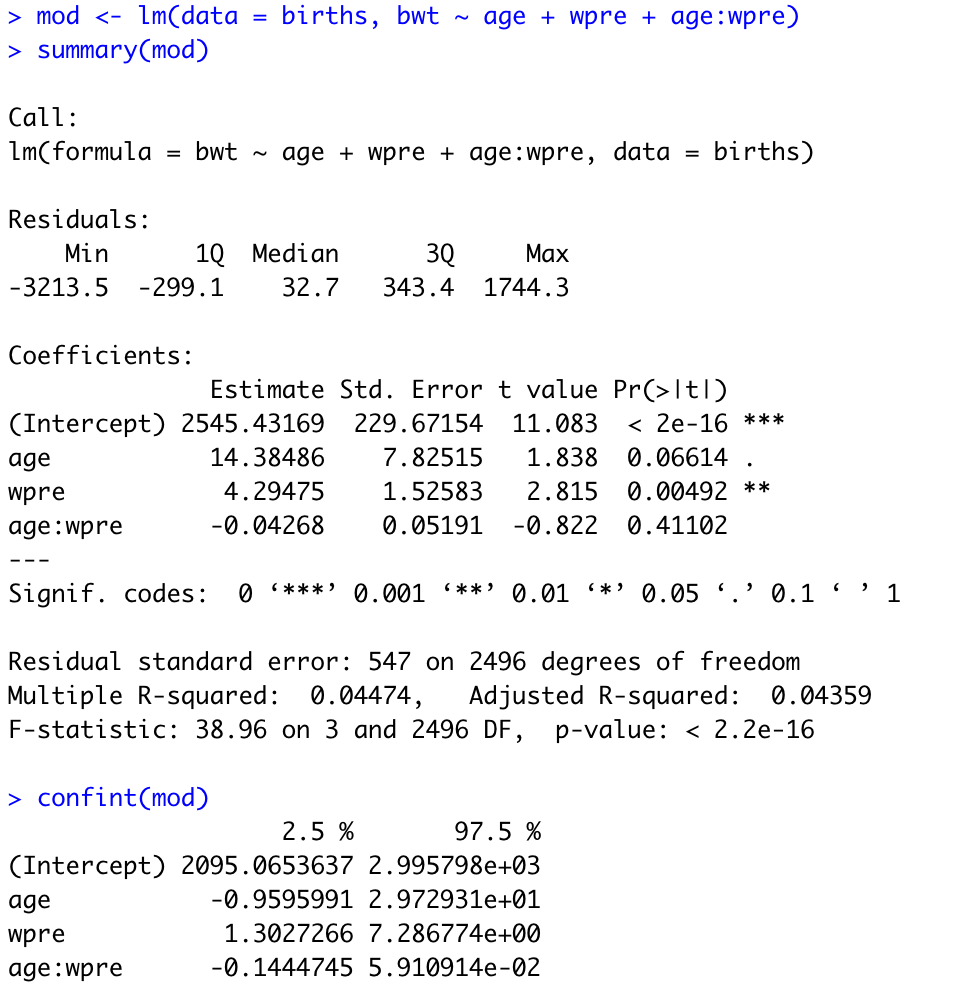
\includegraphics[scale=0.37]{figures/effectmod2.png}
%\end{frame}
%
%\begin{frame}{Effect modification: Another example}
%The coefficient for our interaction term is -0.04 with confidence interval given by (-0.14, 0.06)
%
%\vspace{0.3cm}
%
%\textcolor{blue}{Question:} How do we interpret this interaction term coefficient in our regression model, in the context of our scientific question? \pause
%
%\vspace{0.3cm}
%\textcolor{cyan}{We estimate that among birth parents with one additional pound of pre-pregnancy weight, the difference in average birthweight between groups of parents one year apart in age is 0.04 grams lower, compared to birth parents with one less pound of pre-pregnancy weight. This observed difference in association would not be surprising if the true difference were between -0.14 and 0.06 grams (p = 0.41).}
%
%\end{frame}
%
%\subsection{Precision variables}
%
%% definition slide and example of diagram
%\begin{frame}{Precision variables}
%Causal diagrams can also help us determine whether or not variables are precision variables.
%
%\vspace{0.3cm}
%
%\textcolor{blue}{Precision variable}: a variable that causally affects the outcome \textit{in the population}, but is not associated with the predictor of interest \textit{in the sample} \pause
%
%\vspace{0.3cm}
%
%In a causal diagram, we denote precision variables as\dots
%
%\vspace{0.3cm}
%
%\centering 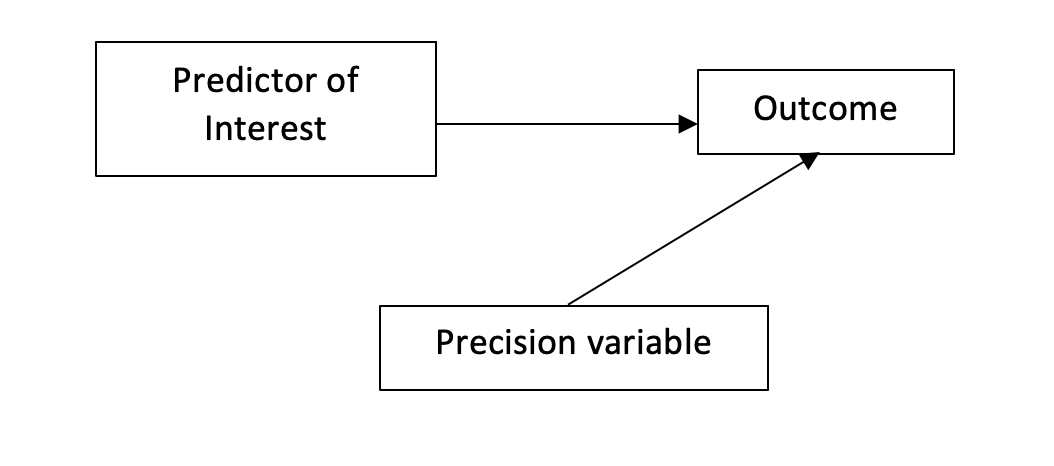
\includegraphics[scale=0.4]{figures/precvar1.png}
%
%\end{frame}
%
%% Example of what to look for graphically in R
%\begin{frame}{Precision variable: what to look for in a graph}
%If your predictor of interest and outcome are both quantitative, and your potential precision variable is \textit{binary}, there are some things you can look for in a graph that may indicate whether or not the potential precision variable is in fact a precision variable. \pause
%
%\vspace{0.3cm}
%
%Below we plot an exposure vs. an outcome:
%
%\vspace{0.1cm}
%
%\centering 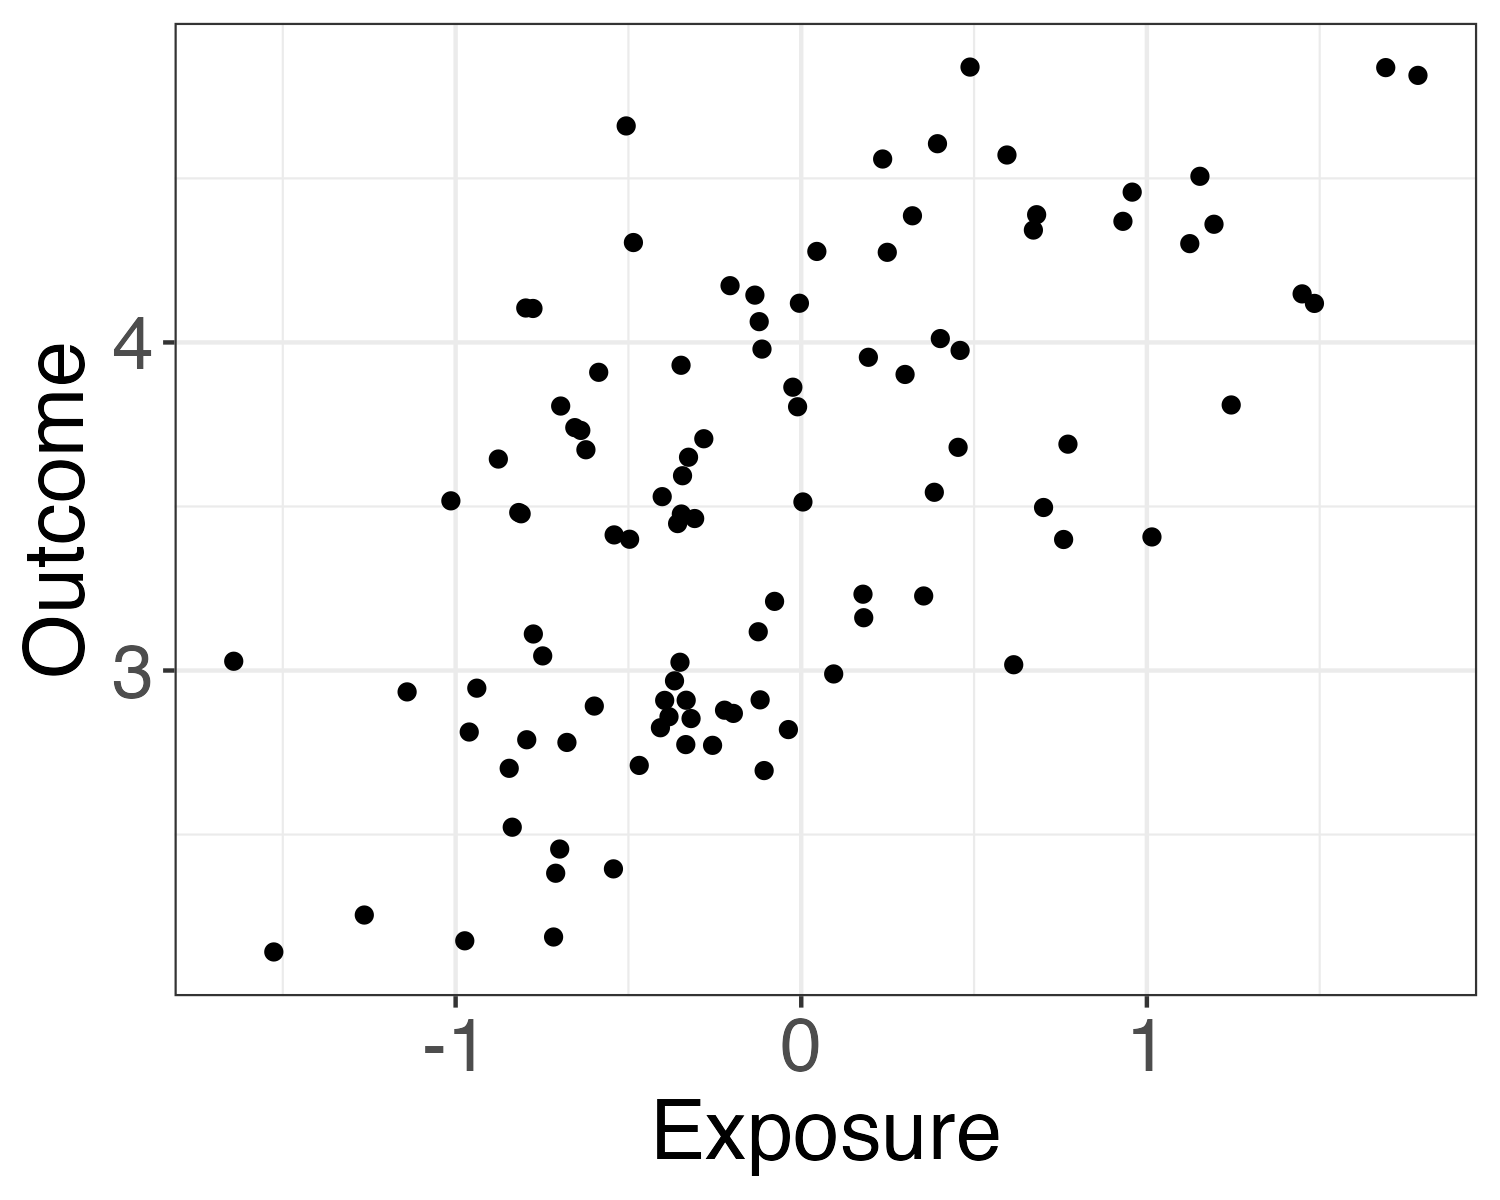
\includegraphics[scale=0.4]{figures/p5.png}
%\end{frame}
%
%\begin{frame}{Precision variables: what to look for in a graph}
%We now color the points by our potential precision variable\dots
%
%\vspace{0.3cm}
%
%\centering 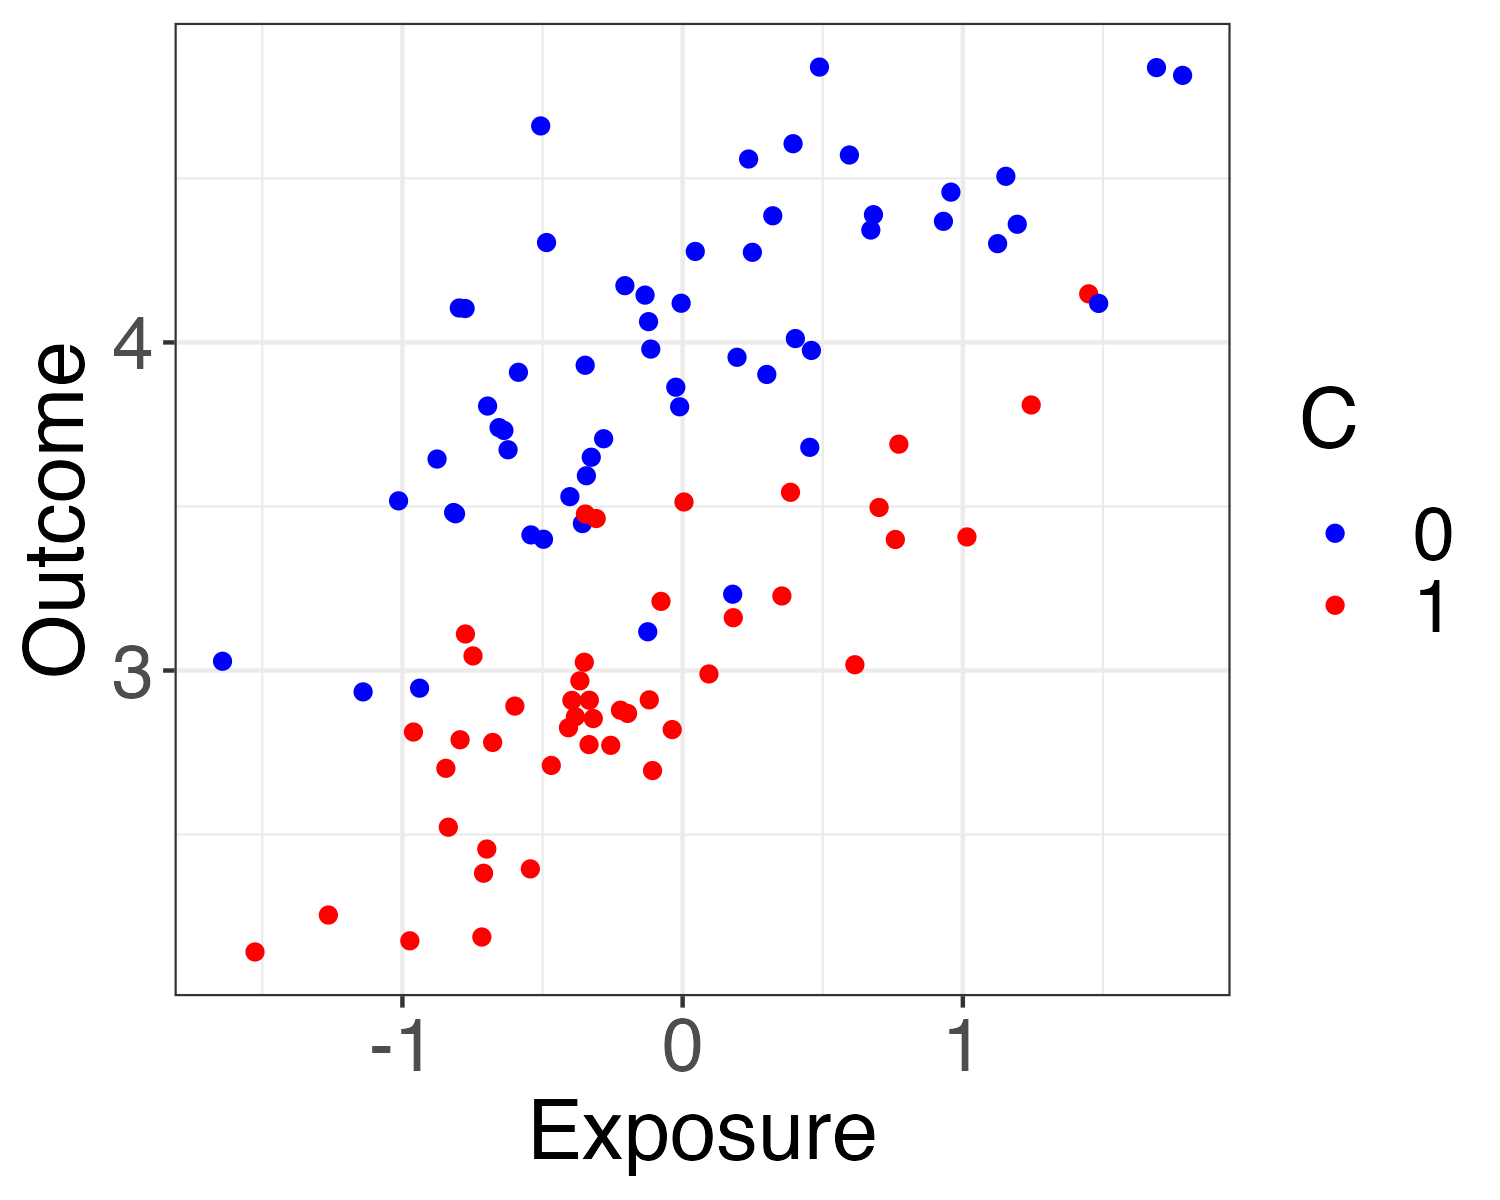
\includegraphics[scale=0.4]{figures/p6.png}
%
%\end{frame}
%
%\begin{frame}{Precision variables: what to look for in a graph}
%\dots and if we were to fit simple linear regressions for each group defined by our potential precision variable (a stratified analysis), we could add those regression lines to the plot as well:
%
%\vspace{0.3cm}
%
%\centering 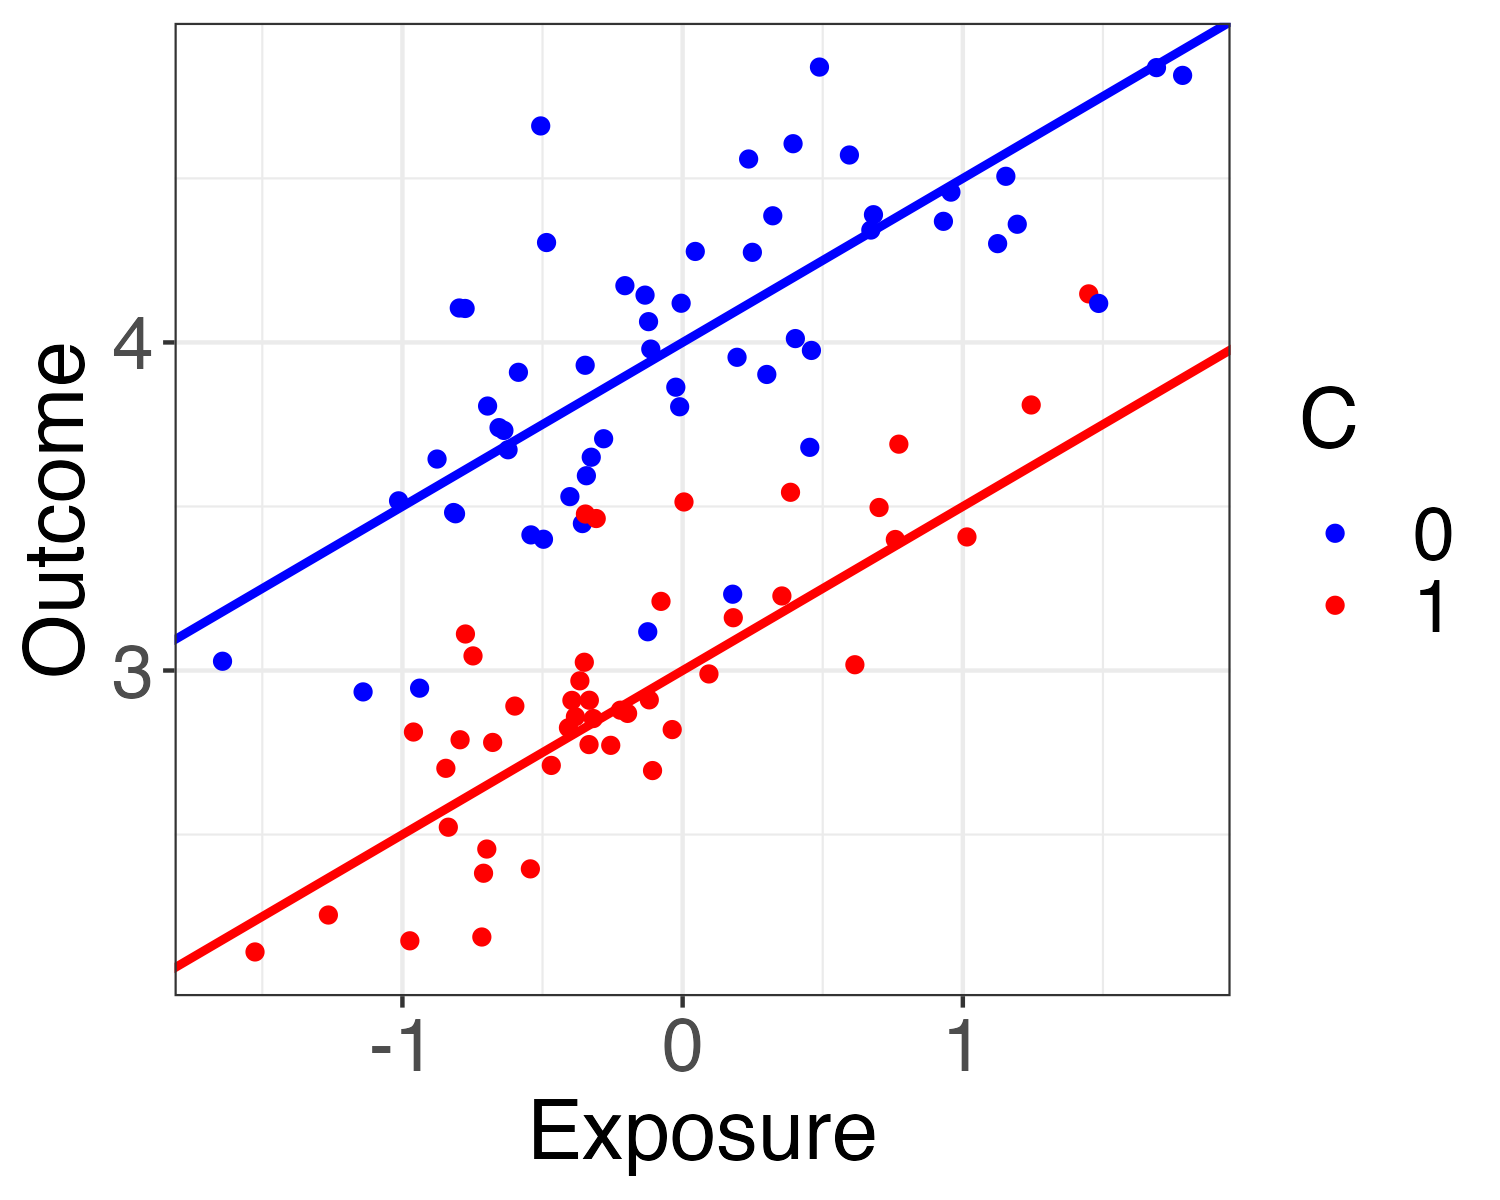
\includegraphics[scale=0.4]{figures/p7.png}
%
%\end{frame}
%
%\begin{frame}{Precision variables: what to look for in a graph}
%	\vspace{-0.5cm}
%\begin{figure}
%	\centering 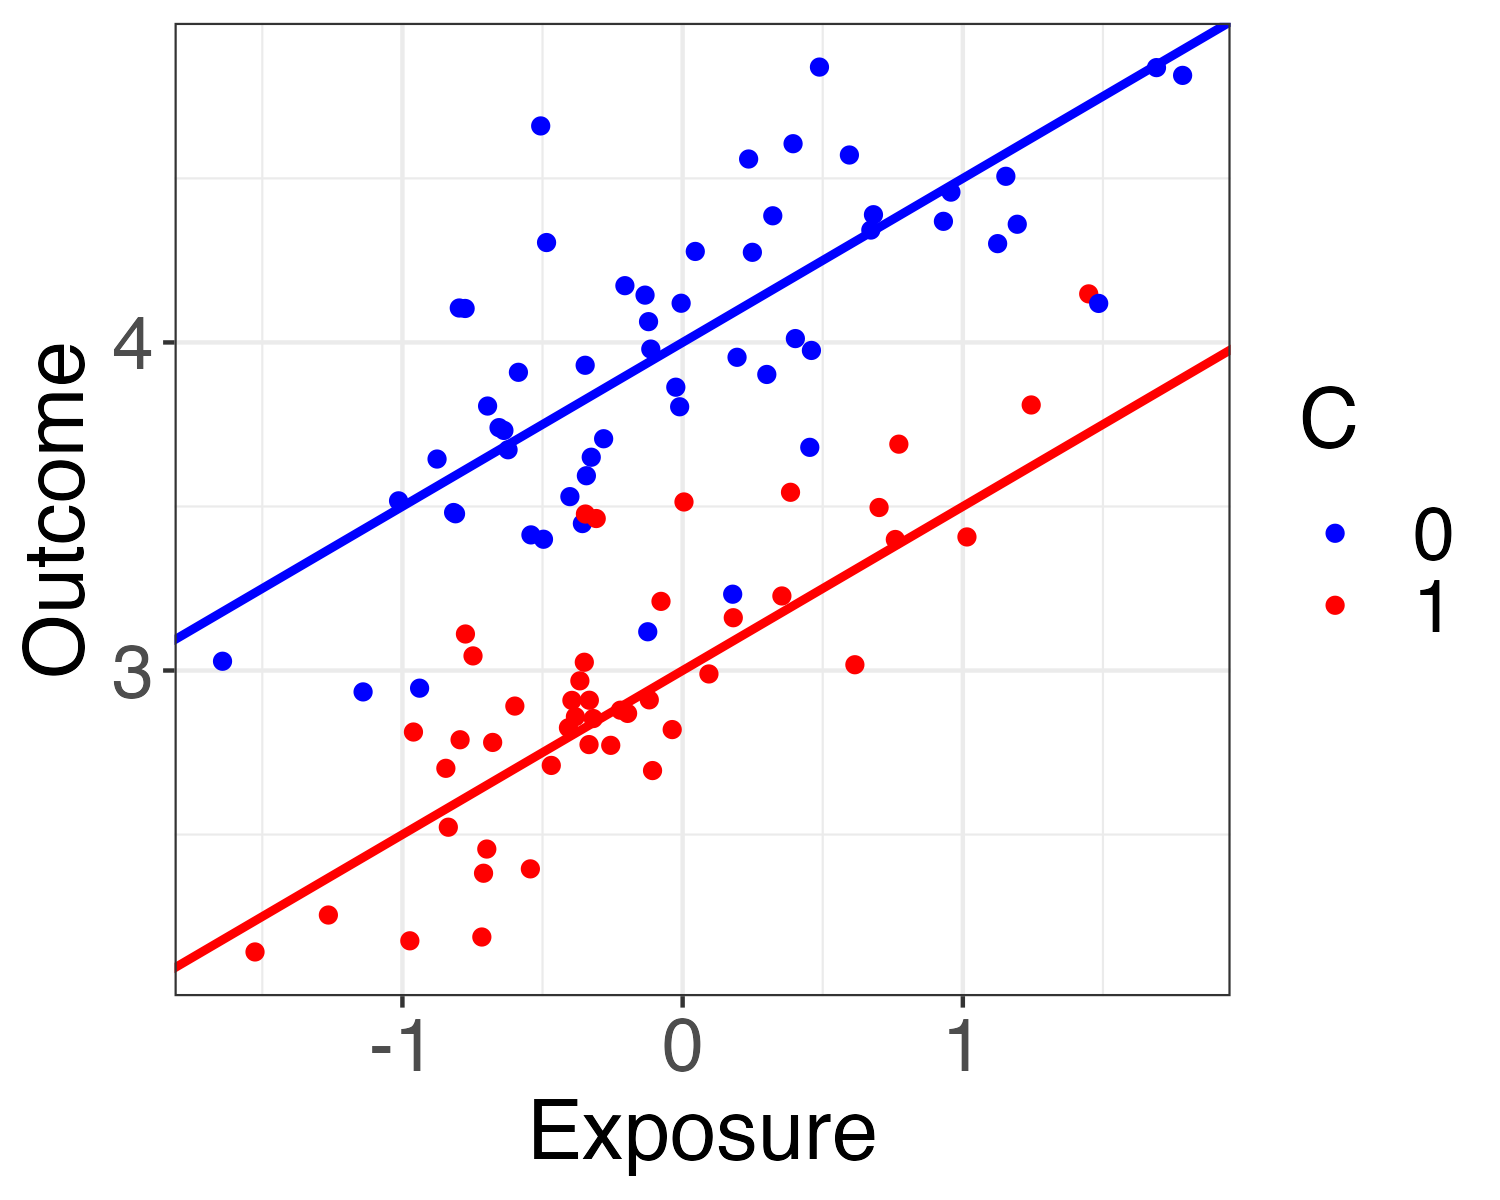
\includegraphics[scale=0.4]{figures/p7.png}
%\end{figure}
%
%\vspace{0.3cm}
%
%The key thing to note here is that the groups defined by a binary precision variable will have linear regression lines with different \textcolor{blue}{intercepts}, but the \textit{same} \textcolor{blue}{slope}. This indicates that there is no association between the exposure and additional variable, and hints that there may be a relationship between the additional variable and the outcome in the population. 
%\end{frame}
%
%\begin{frame}{Precision variables: what to look for in a graph}
%\textcolor{red}{Important note}: A graph alone is not enough to determine if a variable is a precision variable! You still need to think about whether that variable causally affects the outcome \textit{in the population}.
%\end{frame}
%
%\begin{frame}{Precision variables: regression equation}
%Writing regression equations including precision variables is as simple as adding in an additional covariate (just like with confounders). Suppose
%
%\vspace{0.3cm}
%
%\begin{itemize}
%	\item $Y$ = outcome
%	\item $X$ = predictor of interest
%	\item $Z$ = precision variable
%\end{itemize}
%
%\vspace{0.3cm}
%
%Then to include the precision variable $Z$ into our model, we would write
%$$
%E[Y \mid X, Z] = \beta_0 + \beta_1 X + \beta_2 Z
%$$
%
%If we instead had \textit{two} precision variables $Z$ and $W$, we would write
%$$
%E[Y \mid X, Z, W] = \beta_0 + \beta_1 X + \beta_2 Z + \beta_3 W
%$$
%\dots and so forth with additional precision variables!
%
%\end{frame}
%
%\begin{frame}{Precision variables: In \texttt{R}, and interpretation}
%Note that the regression equation for adding potential confounders into a model is the \textit{same} as the regression equation for adding precision variables, in that you only need to add additional variables to the right-hand side of your regression equation.
%
%\vspace{0.3cm}
%
%In \texttt{R}, you do exactly the same things as with confounders, where you simply add another variable to the right-hand side of your formula.
%
%\vspace{0.3cm}
%
%The interpretation of regression coefficients is also the same as for potential confounders, where we interpret each coefficient for a given variable for individuals with \textit{the same} value for all other variables in our model. 
%
%
%\end{frame}
%
%\section{Reivisiting regression assumptions}
%
%\begin{frame}{Revisiting regression assumptions}
%Recall that in Chapter 1a we listed the \textit{classical} linear regression assumptions under the following model
%$$
%Y_i = \beta_0 + \beta_1 X_i + \epsilon_i \text{ for } i = 1, \dots, n
%$$
%as,
%\vspace{0.3cm}
%\begin{itemize}
%	\item \textcolor{red}{L}inearity: There is a linear relationship between $X_i$ and the true population conditional mean $Y_i \mid X_i$
%	\begin{itemize}
%		\item i.e. $E[Y_i \mid X_i] = \beta_0 + \beta_1 X_i$
%	\end{itemize}
%	\item \textcolor{red}{I}ndependence: The errors $\epsilon_i$ are independent of each other
%	\item \textcolor{red}{N}ormality: $\epsilon_i$ are normally distributed
%	\item \textcolor{red}{E}qual variance: $\epsilon_i$ have the same variance
%	\begin{itemize}
%		\item $\epsilon_i \sim N(0, \sigma^2)$, where $\sigma^2$ does not depend on $i$
%	\end{itemize}
%\end{itemize}
%
%\vspace{0.2cm}
%
%\dots however, we learned that when we have large samples, we do not need the normality assumption, and also that the equal variance assumption can be relaxed with the use of robust standard errors
%
%\end{frame}
%
%\begin{frame}{Revisiting regression assumptions}
%For multiple linear regression, we have models with multiple covariates, like this:
%$$
%Y_i = \beta_0 + \beta_1 X_{1,i} + \dots + \beta_p X_{p,i} + \epsilon_i \text{ for } i = 1, \dots, n
%$$
%How do our assumptions change, if at all? \pause
%
%\vspace{0.3cm}
%
%\begin{itemize}
%	\item \textcolor{red}{L}inearity: There is a linear relationship between \color{cyan}$X_{1,i}, \dots, X_{p,i}$ \color{black} and the true population conditional mean \color{cyan}$Y_i \mid X_{1,i}, \dots, X_{p,i}$
%	\begin{itemize}
%		\item i.e. \color{cyan} $E[Y_i \mid X_{1,i}, \dots, X_{p,i}] = \beta_0 + \beta_1 X_{1,i} + \dots + \beta_p X_{p,i}$  \color{black}
%	\end{itemize} 
%	\item \textcolor{red}{I}\color{black}ndependence: The errors $\epsilon_i$ are independent of each other
%	\item \textcolor{red}{N}ormality: $\epsilon_i$ are normally distributed
%	\item \textcolor{red}{E}qual variance: $\epsilon_i$ have the same variance
%	\begin{itemize}
%		\item $\epsilon_i \sim N(0, \sigma^2)$, where $\sigma^2$ does not depend on $i$
%	\end{itemize}
%\end{itemize}
%
%\vspace{0.2cm}
%
%Note that the only assumption that changed, is that we now require a linear relationship between \textit{all covariates} in our model and the true population conditional mean. This assumption can still be checked using the same diagnostic plots as in Chapter 1a!
%
%\end{frame}
%
%
%\begin{frame}{Multiple linear regression: Summary}
%You should now have all the tools you need to:
%
%\vspace{0.3cm}
%\begin{itemize}
%	\item Translate a scientific question into a statistical one that may include \textit{multiple} covariates in a regression model
%	\item Create causal diagrams to help determine the relationship between variables in a model (outcome, predictor of interest, confounder, effect modifier, precision variable)
%	\item Interpret coefficients and confidence intervals in multiple linear regression models (including interaction terms!)
%	\item Use \texttt{R} to fit multiple linear regression models
%	\item Create graphs to support your linear regression analyses
%\end{itemize}
%\end{frame}

\begin{frame}[c]
\centering \huge Any Questions?
\end{frame}

\end{document}